\documentclass{article}
\usepackage[utf8]{inputenc}
\usepackage{amsmath}
\usepackage{afterpage}
\usepackage{amssymb}
\usepackage{svg}
\usepackage{listings}
\usepackage{float}
\usepackage{graphicx,wrapfig,lipsum}
\usepackage[makeroom]{cancel}
\usepackage{blindtext}
\usepackage{multicol}
\usepackage[colorlinks, allcolors=black]{hyperref}


\begin{document}

\begin{titlepage}
    \begin{center}
        \vspace*{1cm}

        \huge
        \textbf{Sistemi elettronici programmabili}

        \vspace{0.5cm}

        Appunti del corso presso l'Università di Pisa

        \vspace{1.5cm}

        \textbf{Aleandro Prudenzano}

        \vfill
        \vspace{0.8cm}

        A.A. 2021-2022

    \end{center}
\end{titlepage}

\clearpage
\begingroup
  \pagestyle{empty}
  \null
  \newpage
\endgroup

\renewcommand{\contentsname}{Indice}
\tableofcontents

\clearpage
\begingroup
  \pagestyle{empty}
  \null
  \newpage
\endgroup
\section{Introduzione}
La crittografia (scrittura nascosta) è lo studio \emph{delle tecniche matematiche per mascherare i messaggi} a differenza della \emph{crittoanalisi} che tenta di svelarli.
Esiste un termine più generico che li comprende: \emph{crittologia}.
Il tipico scenario in cui ci poniamo è quello in cui Alice e Bob vogliono comunicare un messaggio \emph{m} su un canale insicuro in cui è possibile intercettare i messaggi. Decidono quindi di adottare un metodo di cifratura che trasforma m in \emph{c}, detto \emph{crittogramma} che deve essere:

\begin{itemize}
    \item \emph{incomprensibile} al crittoanalista (Eve - Eavesdropper d'ora in poi)
    \item \emph{facilmente decifrabile} da Bob
\end{itemize}

\subsection{Cifratura}
L'operazione con la quale si trasforma m in c è di fatto una funzione:
$$
    C: msg \longrightarrow critto
$$

\subsection{Decifratura}
L'operazione inversa:
$$
    D: critto \longrightarrow msg
$$

\subsection{Schema di comunicazione}
$$
    Alice: m \xrightarrow{C} c \xrightarrow[\text{canale insicuro}]{c} c \xrightarrow{D} m :Bob
$$
Si noti che per funzionare \emph{C} e \emph{D} devono essere in tempo polinomiale mentre per il crittoanalista, noto \emph{c}, deve essere esponenziale il tempo utile per riottenere \emph{m}.
NB: \emph{C} e \emph{D} devono essere l'una l'inversa dell'altra:
$$
    D(c) = D(C(m)) = m
$$
quindi \emph{C} è iniettiva: m diversi vanno in c diversi.

\subsection{Esempi antichi}
Erodoto in "Storie" (V secolo a.C.) scrive:
si prende un servitore, si rasano i suoi capelli e si scrive il messaggio sulla sua testa, si aspetta che la ricrescita lo copra e poi si spedisce il servitore verso Bob che dovrà solamente rasarlo nuovamente.

Gli spartani (V secolo a.C.) usavano lo scitale che è un'asta cilindrica costruita in due esemplari identici posseduti dai due corrispondenti. Su un pezzo di pelle viene scritto il messaggio dopo averlo avvolto attorno al cilindro seguendo le linee di esso. La fettuccia viene poi fatta indossare da un'uomo che la porta al ricevente.

Enea Tattico (Grecia, IV Secolo a.C.) dedica un intero capitolo ai metodi militari usati per scambiarsi i messaggi:
\begin{itemize}
    \item inviare un libro con alcune lettere sottolineate a formare il messaggio in chiaro
    \item sostituire le vocali con altri simboli
\end{itemize}

Cifrario di Cesare: è il più antico cifrario di concezione moderna. \emph{c} è ottenuto da \emph{m} sostituendo ogni lettera con quella a 3 posizioni più avanti:
$$ A \longrightarrow D $$
$$ B \longrightarrow E $$
$$ C \longrightarrow F $$
$$ D \longrightarrow G $$
$$ .. \longrightarrow .. $$
La segretezza in questo caso dipende dalla conoscenza del metodo quindi era destinato ai soli utilizzi ristretti.

\subsection{Livello di segretezza}
I metodi crittografici si classificano in:
\begin{itemize}
    \item \emph{per uso ristretto}: in cui la parte segreta del meccaniscmo è ampia (C e D sono tenute segrete)
    \item \emph{per uso generale}: in cui la parte segreta è molto limitata (si restringe alla sola \emph{chiave}, nota solo ai due endpoint della comunicazione)
\end{itemize}
NB: per i cifrari di massa quindi le regole sono pubblcihe, solo le chiavi sono segrete. Occorre sempre pensare che il nemico conosca il sistema.

Ridefiniamo quindi:
$$ c = C(m, k) $$
$$ m = D(c, k) $$
con \emph{k} chiave segreta diversa per ogni coppia di utenti.
Se non si conosce \emph{k} la conoscenza dell'algoritmo non deve permettere l'estrazione di informazioni dal crittogramma. Se una chiave viene divulgata basta generarne un'altra lasciando inalterati \emph{C} e \emph{D}.
Ovviamente l'insieme delle chiavi deve esere così grande da non essere rompibile tramite brute-force e deve essere scelta in modo casuale.

NB: brute-force $\equiv$ \emph{attacco esauriente}

Es: se |key| = $10^{20}$ ed un calcolatore impiegasse $10^{-6}$ secondi per calcolare $D(c, k)$ e verificarne la significatività occorrerebbero comunque milioni di anni per provarle tutte.
NB: solo la grandezza dello spazio delle chiavi non è un buon indice per l'affidabilità di un cifrario, potrebbe sempre essere rotto matematicamente.

\subsection{Crittoanalisi}
\begin{itemize}
    \item comportamento \emph{passivo}: ci si limita ad ascoltare il canale
    \item comportamento \emph{attivo}: si disturbano le comunicazioni o si modifica il contenuto dei messaggi
\end{itemize}
Gli attacchi dipendono dalle informazioni in possesso del crittoanalista:
\begin{itemize}
    \item \emph{cipher text attack}: si hanno una seria di testi cifrati: $ c_{1}, \_ , c_{r} $
    \item \emph{known plain-text attack}: il crittoanalista ha delle coppie
    $$(m_{1}, c_{1}), \_ , (m_{r}, c_{r})$$
    \item \emph{chosen plain-text attack}: ci si procura una serie di coppie
    $$(m_{1}, c_{1}), \_ , (m_{r}, c_{r})$$
    relative a messaggi in chiaro scelti.
\end{itemize}

\subsection{Attacchi man-in-the-middle}
Il crittoanalista si installa sul canale ed interrompe le comunicazioni dirette tra i due, le sostituisce con messaggi propri e convince ogni utente che quei messaggi provengono legittimamente dall'altro.

\subsection{Situazione attuale}
Si conoscono alcuni \emph{cifrari perfetti} ma richiedono operazioni estremamente complesse, quindi sono utilizzati in condizioni estreme. La definizione di cifrario inattaccabile si deve a \emph{Claude Shannon} ('45 ma pubblicato nel '49). Il messaggio in chiaro ed il crittogramma sono completamente scorrelati tra loro. un esempio è il \emph{one-time pad} che richiede:
\begin{itemize}
    \item una chiave diversa per ogni messaggio
    \item perfettamente casuale
    \item lunga quanto il messaggio
\end{itemize}
Come vanno generate? Come vanno scambiate?
I cifrari utilizzati oggigiorno non sono perfetti ma sono comunque \emph{dichiarati sicuri} perché inviolati e per violarli è necessario risolvere problemi matematici estremamente difficili (abbiamo solo algoritmi esponenziali) quindi è richiesto tanto tempo o calcolatori molto grandi, nella pratica impossibile.

NB: non sempre è noto se l'algoritmo esponenziale è l'unico metodo o ce ne sono altri ancora non scoperti.

Uno dei cifrari di oggi è l'\emph{AES} (Advanced Encryption Standard): è lo standard per le comunicazioni non classificate, pubblicamente noto ed implementabile. Usa chiavi brevi a 128 o 256 bit. E' un cifrario simmetrico a blocchi, la stessa chiave quindi si usa sia per cifrare che per decifrare.

NB: la chiave non è scelta dai partecipanti ma dai compter che usano.
Come trasmettere le chiavi in maniera sicura ed evitare che venga intercettata?

\subsection{Distribuzione delle chiavi}
Nel 1976 è stato proposto un protocollo di creazione e scambio di chiavi su un canale insicuro scenza la necessità che le due parti debbano essersi scambiate altre informazioni. Questo algoritmo è detto \emph{protocollo Diffie-Hellman} acora osa usato largamente.

NB: inventato da Merkle e poi da Diffie ed Hellman

Questi stessi hanno anche creato il concetto di crittografia a chiave pubblica senza tuttavia averne già una implementazione.

\subsection{Cifrari simmetrici ed asimmetrici}
Nei cifrari simmetrici la chiave è unica ed usata sia per criptare che per decriptare ed è nota solo ai due partner che devono averla concordata su un canale sicuro.
Nei cifrari asimmetrici invece si usano una coppia di chiavi:
\begin{itemize}
    \item \emph{$K_{pub}$}: si usa per cifrare, è pubblica e nota a tutti
    \item \emph{$K_{priv}$}: è privata e nota solo a chi riceve.
\end{itemize}
Bisogna quindi creare delle coppie di chiavi per ogni persona che vuole comunicare. Più precisamente:
$$ c = C(m, K_{pub}) $$
$$ m = D(c, K_{priv}) $$
I sistemi simmetrici si dicono anche a chiave privata, mentre quelli asimmetrici si dicono a chiave pubblica.
Per usare un meccanismo come crittografia asimmetrica è necessario l'uso di funzioni \emph{one-way trapdoor} cioè passare da \emph{m} a \emph{c} è facile ma decifrare \emph{c} (senza conoscere la chiave) è difficile.

\subsection{RSA}
Nel 1977 Rivest-Shamir-Adleman inventano un sistema a chiave pubblica basato sulla difficoltà di fattorizzare grandi numeri in fattori primi.
Usando un sistema a chiave pubblica si ha una comunicazione molti a uno in quanto tutti hanno $K_{pub}$ e possono quindi cifrare i messaggi, ma solo il destinatario può leggerli conoscendo $K_{priv}$. Altri vantaggi sono:
\begin{itemize}
    \item tra n persone le chiavi sono $2n$, con un cifrario simmetrico invece sarebbero $\frac{n(n-1)}{2}$
    \item non è necessario lo scambio segreto di chiavi
\end{itemize}

Tuttavia sono molto più lenti e le chiavi sono molto lunghe. Sono soggetti ad attacchi di tipo testo in chiaro scelto.

\subsection{Cifrari ibridi}
Si usa un cifrario a chiave segreta per la comunicazione di massa ma la chiave viene scambiata tramite cifrari asimmetrici. Si hanno quindi:
\begin{itemize}
    \item chiavi piccole
    \item chiave simmetrica randomica impossibile da prevedere tramite attacco di tipo testo in chiaro scelto
\end{itemize}

\subsection{Applicazioni moderne}
Attualmente i protocolli crittografici sono usati anche per:
\begin{itemize}
    \item \emph{identificazione dell'utente}: si accerta l'identità
    \item \emph{autenticazione dell'utente}: si accerta che il messaggio venga dalla persona che dice di averlo mandato
    \item \emph{firma digitale}: permette di evitare che un utente che ha inviato un messaggio neghi di averlo fatto e si dimostra l'identità del mittente agli occhi del ricevente
\end{itemize}

\subsection{Svolte future}
\begin{itemize}
    \item trasmissione protetta sulla rete (OpenSSL)
    \item moneta elettronica (protocollo Bitcoin)
    \item protocolli zero-knowledge
    \item protocolli di cifratura quantistici
\end{itemize}
\section{Rimandi alla teoria dell'informazione}
\subsection{Rappresentazione matematica di oggetti}
Un \emph{alfabeto} è un insieme finito di caratteri detti simboli. Un oggetto è rappresentato da una sequenza ordinata di caratteri dell'alfabeto. A oggetti diversi corrispondono sequenze diverse ed il numero di oggetti rappresentabili è infinito (fissata una lunghezza qualsiasi posso sempre creare sequenze più lunghe). 
Fissato un alfabeto $\Gamma$ tale che $|\Gamma| = s$ e fissati \emph{N} oggetti da rappresentare:
\begin{itemize}
    \item $d(s, N)$: è la lunghezza della sequenza più lungha di un oggetto dell'insieme
    \item $d_{min}(s, N)$: valore minimo di $d(s, N)$ tra tutte le rappresentazioni possibili
\end{itemize}

NB: un metodo di rappresentazione è tanto migliore tanto più $d(s, N)$ si avvicina a $d_{min}(s, N)$.

Es: s = 1, $\Gamma = \{0\}$: per creare oggetti diversi vario la lunghezza della sequenza: 0, 00, ecc. Per N oggetti quindi $d_{min}(s, N) = N$

Es: s = 2, $\Gamma = \{0, 1\}$: $\forall k \geq 1$ si hanno $2^{k}$ sequenze di lunghezza $k$ quindi il numero totale di sequenze lunghe da 1 a k è:
$$
    \sum^{k}_{i=1} 2^{i} = 2^{k+1} - 2
$$
per N oggetti da rappresentare quindi:
$$
    2^{k+1} - 2 \geq N \implies K \geq log_{2}(N+2) - 1
$$
quindi
$$ d_{min}(2, N) = \lceil log_{2}(N+2) - 1 \rceil $$
$$ \lceil log_{2}N \rceil - 1 \leq d_{min}(2, N) \leq \lceil log_{2}N \rceil $$

Es: $N = 7$, $\lceil log_{2}7 \rceil = 3$ quindi \{0, 1, 00, 01, 10, 11, 000\}

NB: posso costruire $N$ sequenze differenti tutte di $ \lceil log_{2}N \rceil $ caratteri: {000, 001, 010, 011, 100, 101, 110}. Questo vale per tutti gli $s$ quindi:
\begin{itemize}
    \item posso costruire N sequenze differenti con $ \lceil log_{2}N \rceil $ caratteri
    \item posso costruire N sequenze differenti tutte di $ \lceil log_{2}N \rceil $ caratteri
\end{itemize}

Es: $\Gamma = \{0, \_, 9 \}$ $\implies$ $\lceil log_{10}1000 = 3 \rceil$ cioè i numero da 000 a 999

Usare sequenze tutte della stessa lunghezza è vantaggioso perché posso concatenare più oggetti senza usare un separatore. Si dice \emph{rappresentazione efficiente} una rappresentazione che usa un numero massimo di caratteri di ordine logaritmico nella cardinalità dell'insieme da rappresentare (N) quindi bisogna avere almeno 2 caratteri.

\subsection{Rappresentazione di interi}
La notazione posizionale per gli interi è efficiente indipendentemente dalla base $s \geq 2$ scelta perché un intero N di d cifre soddisfa : $\lceil log_{2}N \rceil \leq d \leq \lceil log_{2}N \rceil + 1$

\subsection{Teoria della calcolabilità}
Si occupa delle questioni circa la potenza e le limitazioni dei sistemi di calcolo. Si parte dalla prima metà del XX secolo con l'esplorazione della computazione, degli algoritmi, dei problemi risolvibili per via algoritmica e si dimostra anche l'esistenza di problemi che non ammettono un algoritmo di risoluzione: \emph{i problemi non decidibili}.

\subsubsection{Problemi computazionali}
Sono problemi formulati matematicamente di cui cerchiamo una soluzione algoritmica. Vengono classificati in:
\begin{itemize}
    \item \emph{problemi non decidibili}
    \item \emph{problemi decidibili}: tutti i problemi risolvibili con un algoritmo indipendentemente dal tempo. Di questo si occupa la teoria della complessità dividendoli in:
    \begin{itemize}
        \item \emph{trattabili} (costo polinomiale)
        \item \emph{non trattabili} (costo esponenziale)
    \end{itemize}
\end{itemize}

\subsubsection{Esistenza di problemi non decidibili}
Due insiemi $A$ e $B$ hanno la stessa cardinalità \emph{se e solo se} si può stabilire una corrispondenza biunivoca tra i loro elementi (una mappa).
Un insieme è \emph{numerabile} (ha una infinità numerabile di elementi) \emph{se e solo se} i suoi elementi si possono mettere in corrispondenza biunivoca con i numeri naturali.

NB: un insieme numerabile può essere elencato: $a_1, a_2, \_, a_n, \_ $
NB: sono numerabili anche le stringhe di lunghezza finita di simboli di un alfabeto finito

Si vogliono elencare le sequenze in un ordine ragionevole, non possiamo quindi usare l'ordine lessicografico perché non si può completare l'elenco. Per trovare un elenco che soddisfi la numerabilità dobbiamo:
\begin{itemize}
    \item raggiungere qualsiasi sequenze $\sigma$ scelta in un numero \emph{finito} di passi
    \item $\sigma$ deve quindi trovarsi a distanza \emph{finita} dall'inizio dell'elenco
\end{itemize}

Useremo quindi l'\emph{ordinamento canonico}:
\begin{itemize}
    \item si ordinano le sequenze per lunghezza crescente
    \item le sequenze di pari lunghezza si ordinano alfabeticamente (supponendo di avere creato una regola di ordine tra i caratteri)
\end{itemize}

Quindi una sequenza $s$ si trova tra quelle $|s|$.

Es: $\Gamma = \{ a, b, c, \_, z \} \implies a, b, \_, z, aa, ab, \_, zz, aaa, \_ $

Seguendo questo metodo ogni sequenza corrisponde ad un numero $\in \mathbb{N}$ ed ogni naturale ha una sequenza associata.

NB: questo si può fare perché abbiamo preso sequenze di lunghezza finita, per sequenze di lunghezza infinita non esiste una enumerazione.

Alcuni esempi di insiemi non numerabili sono:
\begin{itemize}
    \item $\mathbb{R}$
    \item $\mathbb{R}$ ristretto a $(0, 1)$ o $[0, 1]$
    \item insieme delle funzioni in una o più variabili
\end{itemize}

Dimostriamo l'appartenenza di quest'ultimo: un problema computazionale può essere visto come una funzione matematica che associa ad ogni insieme di dati su $k$ numeri interi il risultato su $j$ numeri interi:
$$ f :  \mathbb{N}^{k} \longrightarrow \mathbb{N}^{j} $$

Dimostriamolo su un sott'insieme $F = \{f | f: \mathbb{N} \longrightarrow \{0, 1\}\}$. Ogni $f \in F$ può essere rappresentata da una sequenza infinita:
\begin{table}[!h]
    \centering
    \begin{tabular}{c|c|c|c|c|c|c|c}
         $x$ & 0 & 1 & 2 & 3 & \_ & n & \_  \\
         \hline
         $f(x)$ & 0 & 1 & 0 & 1 & \_ & 0 & \_
    \end{tabular}
\end{table}

oppure da una regola finita di costruzione:

\begin{equation}
    f(x) =
    \begin{cases}
        $0 \text{se x è pari}$ \\
        $1 \text{se x è dispari}$
    \end{cases}
\end{equation}

Supponiamo per assurdo che $F$ sia numerabile, quindi è possibile trovare una enumerazione per $f \in F$:
\begin{table}[!h]
    \centering
    \begin{tabular}{c|c c c c}
        $x$ & 0 & 1 & 2 & \_  \\
        \hline
        $f_0(x)$ & 1 & 0 & 1 & \_ \\ 
        $f_1(x)$ & 0 & 0 & 1 & \_ \\ 
        $f_2(x)$ & 1 & 1 & 0 & \_ \\ 
    \end{tabular}
\end{table}

Consideriamo dunque la seguente funzione:

\begin{equation}
    g(x) = 
    \begin{cases}
        $0 \text{ se }$ f_x(x) = 1 \\
        $1 \text{ se }$ f_x(x) = 0 \\
    \end{cases}
\end{equation}

$g \in F$ perché è una funzione dai naturali a \{0, 1\} ma non può corrispondere a nessuna delle funzioni nella tabella precedente.
\begin{itemize}
    \item non può essere $f_0$ in quanto differisce in $x = 0$
    \item non può essere $f_1$ in quanto differisce in $x = 1$
    \item e così via $\forall n$
\end{itemize}
La nostra tabella, e quindi $F$ ha almeno una funzione mancante. Supponiamo ancora per assurdo che $\exists j \text{ tc } g(x) = f_{j}(x)$ quindi:
\begin{itemize}
    \item $g(x) = 1$ se $f_j(x) = 0$ ma $g(x)=f_j(x)$ 
    \item $g(x) = 0$ se $f_j(x) = 1$ ma $g(x)=f_j(x)$ 
\end{itemize}
siamo ad un assurdo $\implies$ l'insieme delle funzioni $f: \mathbb{N} \longrightarrow \{0, 1\}$ è non numerabile, quindi lo è anche l'insieme che le comprende $f:\mathbb{N}^{k} \longrightarrow \mathbb{N}^{j}$.

\emph{L'insieme dei problemi computazionali non è numerabile}.

\subsubsection{Il problema della rappresentazione}
L'informatica rappresenta tutte le sue entità in forma digitale come sequenze finite di simboli finiti. Possiamo dire quindi che la conoscenza umana è numerabile.

\subsubsection{Algoritmo}
E' una sequenza finita di operazioni, completamente e univocamente determinate. La formulazione di un algoritmo dipende dal modello di calcolo utilizzato: se uso la macchina di Turing ho una codifica, se uso il C ne ho un'altra, ecc. Qualsiasi codifica si scelga però gli algoritmi devono essere sempre descritti da una sequenza finita di caratteri di un alfabeto finito.

\emph{Gli algoritmi sono infiniti ma numerabili, i problemi sono infiniti ma non numerabili quindi esistono problemi privi di un corrispondente algoritmo di calcolo}.

\subsubsection{Problema dell'arresto (Halt problem)}
Alan Turing nel 1930 scopre il problema dell'arresto e dimostra essere non decidibile. E' un problema decisionale, cioè:
$$ HLT:\{Istanze\} \longrightarrow \{0, 1\} $$
quindi la calcolabilità p chiamata \emph{decidibilità}.

\emph{Presi arbitrariamente un algoritmo A ed i suoi dati di input D, decidere in tempo finito se la computazione di A su D termina o no}.

Si cerca quindi un algoritmo che indaghi le proprietà di un altro algoritmo usato come input. (Si può fare perché algoritmi e dati sono rappresentati come sequenze di caratteri dello stesso alfabeto). Un test di primalità termina, un algoritmo che cerca un numero che fallisce alla congettura di Goldbach (ogni numero intero pari $\geq 4$ può essere espresso come somma di due primi) non sappiamo se termina o meno in quanto non sappiamo se la congettura sia vera o meno:
$$ \text{congettura falsa} \longrightarrow \text{l'algoritmo termina} $$
$$ \text{congettura vera} \longrightarrow \text{l'algoritmo non termina} $$

\subsubsection{Indecidibilità del problema dell'arresto}
Supponiamo per assurdo che il problema sia decidibile, quindi esiste un algoritmo $ARRESTO$ che presi A e D determini in tempo finito la risposta.
Questo algoritmo non può essere una mera simulazione di A su D in quanto se A termina il risultato è positivo, se A non termina l'algoritmo non può dire in tempo finito che A non termina. $ARRESTO$ deve quindi osservare A dall'esterno. Scegliamo quindi $D=A$ e consideriamo $A(A)$:
$$ A(A) = 1 \Longleftrightarrow A(A) termina $$
costruiamo allora un secondo algoritmo:
\begin{verbatim}
    PARADOSSO(A){
        while(ARRESTO(A, A));
    }
\end{verbatim}
quindi $PARADOSSO(A)$ termina se e solo se $A(A)$ non termina.
Calcoliamo quindi $PARADOSSO(PARADOSSO)$, cosa succede?

Termina se e solo se $ARRESTO(PARADOSSO) = 0$ cioè se e solo se $PARADOSSO(PARADOSSO)$ non termina.
Abbiamo una contraddizione quindi se ne ottiene che non può esistere l'algoritmo $ARRESTO$ e dunque il problema dell'arresto è indecidibile.

\subsubsection{Altri problemi indecidibili}
E' indecidibile stabilire l'equivalente tra due programmi (stesso input $\implies$ stesso output).
In genere non esistono algoritmi che decidono il comportamento di altri algoritmi senza passare dalla loro simulazione. E' indecidibile il problema della ricerca di soluzione di equazioni diofantee di grado arbitrario.

\subsubsection{Modelli di Calcolo}
La teoria della calcolabilità dipende dal modello di calcolo? Oppure è una proprietà del problema? I linguaggi di programmazione sono tutti equivalenti? Ce ne sono di più potenti o semplici di altri? Ci sono algoritmi scrivibili in un linguaggio ma non in un altro? In futuro alcuni problemi indecidibili diventeranno decidibili con nuovi paradigmi o nuovi calcolatori? Non lo sappiamo. La tesi di \emph{Church-Turing} ci dice che \emph{tutti i modelli di calcolo risolvono esattamente la stessa classe di problemi}, quindi si equivalgono pur operando con diversa efficienza e la decidibilità è una proprietà del problema. Tuttavia non è dimostrato per ora.

\subsubsection{Trattabilità}
Dopo i problemi indecidibili ci sono i problemi \emph{intrattabili} cioè quei problemi che hanno come limite inferiore per i tempi di risoluzione un esponenziale nella dimensione dell'istanza. Successivamente vi sono i problemi \emph{trattabili} cioè problemi con costo polinomiale. In fine c'è una famiglia di cui non si conosce lo stato, il costo. Abbiamo algoritmi esponenziali ma non sappiamo i limiti inferiori di questi problemi. Li chiamiamo \emph{presumibilmente intrattabili}.

Studiamo la dimensione dei dati trattabili in funzione dell'incremento della potenza dei calcolatori. Sia dato $C_{1}$ con una velocità e $C_{2}$ con $k$ volte la velocità di $C_{1}$. Su un tempo di calcolo $t$:
$$ n_{1} = \text{dati trattabili su $C_{1}$ in tempo $t$} $$
$$ n_{2} = \text{dati trattabili su $C_{2}$ in tempo $t$} $$
quindi usare $C_{2}$ per t equivale ad usare $C_{1}$ per $k \cdot t$.
Sia dato un algoritmo polinomiale che si risolve in $c \cdot n^{s}$ secondi (con c, s costanti) si hanno:
$$ c_{1}: c \cdot n_{1}^{s} = t \longrightarrow n_{1} = \left( \frac{t}{c} \right)^{\frac{1}{s}} $$
$$ c_{2}: c \cdot n_{2}^{s} = k \cdot t \longrightarrow n_{2} = \left(\frac{k \cdot t}{c}\right)^{\frac{1}{s}} = k^{\frac{1}{s}} \cdot \left( \frac{t}{c} \right) ^{\frac{1}{s}} = k^{\frac{1}{s}} \cdot n_{1} $$
il miglioramento è di un fattore moltiplicativo di $k^{\frac{1}{s}}$.

Sia ora dato un algoritmo esponenziale che si risolve in $c \cdot 2^n$ (con c costante)
$$ c_{1}: c \cdot 2^{n_{1}} = t \longrightarrow 2^{n_1} = \frac{t}{c} $$
$$ c_{2}: c \cdot 2^{n_{2}} = k \cdot t \longrightarrow 2^{n_2} = k \cdot \frac{t}{c} = k \cdot 2^{n_1} \implies n_2 = n_1 + log_{2}k $$
Il miglioramento è di un fattore additivo logaritmico!

NB: se prima si trattavano problemi di istanza 1000 dopo essere passati ad una macchina più potente con $k = 10^9$ si potranno trattare istanze $1000 + log_2{10^9} \approx 1030$. Questo è il motivo per il quale si distingue tra trattabili ed intrattabili!

\subsubsection{Problemi}
Dato un problema $\Pi$ indichiamo con:
\begin{itemize}
    \item $I$: insieme delle \emph{istanze} di ingresso
    \item $S$: insieme delle \emph{soluzioni}
\end{itemize}
Alcune tipologie di problemi sono:
\begin{itemize}
    \item \emph{problemi decisionali} se $S = \{0, 1\}$ (un numero è primo? un grafo è connesso?). Chiamiamo $x \in I$ istanza positiva o accettabile se $\Pi(x) = 1$ ed istanza negativa se: $\Pi(x) = 0$
    \item \emph{problemi di ricerca} se dato $x \in I$ ci fornisce una soluzione $s$ (trovare un cammino tra due vertici, ecc)
    \item \emph{problemi di ottimizzazione} se dato $x \in I$ si vuole trovare la migliore soluzione $s$ tra tutte quelle ammissibili (cammino minimo, ecc)
\end{itemize}
La teoria della complessità fa riferimento alla sola classe decisionale in quanto:
\begin{itemize}
    \item essendo $s = \{0, 1\}$ non ci si deve preoccupare del tempo per restituire la soluzione
    \item la difficoltà è già presente nella sua versione decisionale
    \item ogni problema di ottimizzazione può essere espresso in forma decisionale chiedendo l'esistenza di una soluzione che soddisfi una certa proprietà
    
    Es: \emph{trovare la clique più grande in G} (ottimizzazione) diventa \emph{esiste una clique in G di almeno k vertici?} (decisionale).
    
    La seconda in particolare non può essere più difficile della prima, se lo fosse potremmo usare la prima per cercare una soluzione e controlliamo rispetto alla dimensione k, ergo dal primo al secondo è immediato!
    Il problema di ottimizzazione è tanto difficile quanto la sua versione decisionale, studiando il secondo posso quindi fornire un limite inferiore alla versione di ottimizzazione.
\end{itemize}

\subsubsection{Classi di complessità}
Dato $\Pi$ decisionale ed A algoritmo diciamo che A risolve $\Pi$ se, dato l'input $x$:
$$ A(x) = 1 \Longleftrightarrow \Pi(x) = 1 $$
Diciamo poi che A risolve $\Pi$ in tempo $t(n)$ ed in spazio $s(n)$ se il tempo di esecuzione e l'occupazione di memoria di A sono $t(n)$ e $s(n)$. Dato $f(n)$ diremo:
\begin{itemize}
    \item $Time(f(n))$ è l'insieme dei problemi decisionali che possono essere risolti in tempo $O(f(n))$
    \item $Space(f(n))$ è l'insieme dei problemi decisionali che possono essere risolti in spazio $O(f(n))$
\end{itemize}

\subsubsection{Classe P}
E' la classe di problemi che possono essere risolti in tempo polinomiale nella dimensione dell'istanza di input.

NB: un algoritmo è polinomiale se $\exists c, n_0 > 0 $ tale che il numero di passi elementari è al più $n^c$ per ogni input di dimensione $n \forall n > n_0$.

Esiste l'analogo nello spazio e lo indichiamo con $PSPACE$

\subsubsection{Classe EXP-TIME}
La classe Exp(time) è la classe dei problemi risolvibili in tempo esponenziale nella dimensione $n$ dell'istanza di input.

NB: $P \subseteq Exp-Time$

NB: $P \subseteq PSpace$ perché un algoritmo polinomiale può accedere al più ad un numero polinomiale di locazioni di memoria (altrimenti dovrebbe essere esponenziale).

NB: $PSpace \subseteq Exp-Time$

Ad oggi non sappiamo se sono inclusioni proprie, l'unica separazione netta è $P \subset Exp-Time$ poiché abbiamo problemi risolti in $Exp$ e non in $P$ (ad esempio Hanoi)

\subsubsection{SAT}
Sia dato un insieme V di variabili logiche, definiamo:
\begin{itemize}
    \item letterale: una variabile o una sua negazione
    \item clausola: disgiunzione (OR) di letterali
    \item espressione booleana in forma normale congiuntiva (FNC): è una espressione logica formata da clausole unite da congiunzioni (AND di OR di variabili dirette o negate)
    
    Es: dati $ V = \{x, y, z, w\}$ una possibile FNC potrebbe essere: 
    $$(x \lor \bar{y} \lor z) \land (\bar{x} \lor w) \land y$$
\end{itemize}

SAT si occupa di cercare dei valori di verità per rendere vera l'espressione.

Es: è soddisfatta per $x=1, y=1, z=0, w=1$

NB: il problema c'è solo se l'espressione è FNC e passare ad un'altra forma richiede tempo esponenziale.

Per risolvere iteriamo sulle $2^n$ possibili combinazioni e controlliamo la soddisfattibilità.

$$ SAT \in Exp-Time$$
quindi per risolvere questo ed altri problemi (clique, cammino hamiltoniano) è necessario iterare tra tutte le possibili combinazioni di ingresso? \emph{Non lo sappiamo}. Da qui parte la questione $P$ vs $NP$.

\subsubsection{Certificati}
In un problema decisionale siamo interessati a verificare se un'istanza del problema soddisfa una certa proprietà. Per alcuni problemi, per le istanze accettabili è possibile fornire un certificato che ci convinca della sua accettabilità.

Es: certificato per clique: sottoinsieme di k vertici che forma la clique. Certificato per cammino hamiltoniano: la permutazione degli n vertici che definisce il cammino.

Quando ho un certificato posso controllarlo in tempo polinomiale ed accertarmi che sia vero.

E' di fatto un attestato \emph{breve} di esistenza di una soluzione. Si definisce solo per le istanze accettabili perché in genere non è facile costruire certificati di non esistenza.

Es: $UNSAT$: è vero che nessun assegnamento rende vera l'espressione? Per questo problema non basta fornire un assegnazione accettabile, non sarebbe breve!

\subsubsection{Teoria della verifica}
Utiliziamo il costo della verifica di un certificato per una istanza positiva per caratterizzare la complessità del problema stesso. Un problema $\Pi$ è \emph{verificabile in tempo polinomiale} se
\begin{itemize}
    \item ogni istanza accettabile $x$ di $\Pi$ di lunghezza $n$ ammette un certificato $y$ di lunghezza polinomiale in $n$
    \item esiste un algoritmo di verifica polinomiale in $n$ ed applicabile ad ogni coppia $<x$, $y>$ che attesta se $x$ è accettabile.
\end{itemize}


\subsubsection{Classe NP}
NP è la classe dei problemi decisionali verificabili in tempo polinomiale.

NB: NP sta per \emph{polinomiale su macchine non deterministiche}

Abbiamo quindi che se si ha una soluzione essa è facile da verificare ma se non si ha una soluzione la si cerca in tempo esponenziale.

\subsubsection{P vs NP}
$P \subseteq NP$ certamente perché qualsiasi problema in P può essere risolto in tempo polinomiale. Non sappiamo però se $P \subset NP$ o $P = NP$


\subsubsection{Problemi NP-completi}
Sono i problemi più difficili dentro NP: se esistesse un algoritmo polinomiale per risolvere uno solo di questi allora tutti i problemi in NP sarebbero risolti in tempo polinomiale $\implies$ P = NP. Quindi o tutti i problemi NP-completi si risolvono in tempo polinomiale oppure nessuno lo è.

\subsubsection{Riduzioni polinomiali}
Presi $\Pi_{1}$ e $\Pi_{2}$ problemi decisionali, $I_{1}$ e $I_{2}$ insiemi degli input di $\Pi_{1}$ e di $\Pi_{2}$ diremo che $\Pi_{1}$ si riduce in tempo polinomiale a $\Pi_{2}$:
$$ \Pi_{1} \leq_{p} \Pi_{2} $$
se esiste una funzione $f:I_{1} \longrightarrow I_{2}$ calcolabile in tempo polinomiale tale che mi trasforma una istanza del primo problema in una istanza del secondo e $\forall x \in \Pi$:
$$ x \text{ è accettabile per } \Pi_{1} \Longleftrightarrow f(x) \text{ è accettabile per } \Pi_{2} $$

E' utile perché supponendo di risolvere $\Pi_{2}$ in tempo polinomiale allora $\Pi_{1}$ viene tradotto in tempo polinomiale in $\Pi_{2}$ e quindi anche $\Pi_{1}$ è polinomiale:
$$ \Pi_{1} \leq_{p} \Pi_{2} \text{ e } \Pi_{2} \in P \Longrightarrow \Pi_{1} \in P $$

\subsubsection{Np arduo}
Un problema $\Pi$ si dice NP-arduo se:
$$ \forall \Pi' \in NP \text{  } \Pi_{1}' \leq_{p} \Pi $$

NB: $\Pi$ non per forza decisionale

\subsubsection{NP-completo}
Un problema decisionale $\Pi$ si dice NP-completo se:
$$ \Pi \in NP $$
$$ \forall \Pi' \in NP \text{  } \Pi' \leq_{p} \Pi $$
Dimostriamo che se trovo $\Pi$ NP-completo ma $\Pi \in P$ allora P=NP: per ogni $\Pi' \in NP$ $\Pi' \leq \Pi$ quindi trasformo $I_{\Pi'}$ in $I_{\Pi}$, $I_{\Pi}$ so risolverlo in tempo polinomiale quindi qualunque $\Pi' \in NP$ è risolto in tempo polinomiale.

Dimostrate che $\Pi$ appartiene a NP è facile: si deve esibire un certificato polinomiale. Non è semplice invece dimostrare che un problema è NP-arduo o NP-completo perché:
\begin{itemize}
    \item devo dimostrare che tutti i problemi NP si riducono a $\Pi$
    \item ma la prima definizione di NP-completo aggira il problema: il \emph{Teorema di Cook}
\end{itemize}

\subsubsection{Teorema di Cook}
Dati un qualunque problema NP ed una qualunque istanza $x$ si può dimostrare che una espressione booleana in forma normale congiuntiva che descrive \\ l'algoritmo del problema si può sempre costruire.

Quindi \emph{qualsiasi problema NP si riduce a $SAT$}.
Per dimostrarle quindi che un problema è NP-completo ci basta prenderne uno che lo è e provare a ridurlo al problema in studio.

Es: per dimostrare che clique è NP-completo cerchiamo un algoritmo polinomiale tc:
$$ SAT \leq_{p} CLIQUE $$
se lo troviamo allora $CLIQUE$ è NP-completo. $SAT$ e $CLIQUE$ sono NP equivalenti: \emph{tutti i problemi NP completi sono tra di loro NP equivalenti}.


\subsubsection{Ottimizzazione di problemi NP-hard}
Se la soluzione ottima è troppo difficile da ottenere si opta per una quasi ottima. In particolare ci si accontenta di:
\begin{itemize}
    \item soluzioni che non si discostino troppo da quella ottima
    \item soluzioni che si calcolano in tempo polinomiale
\end{itemize}

\subsubsection{Classi co-P e co-NP}
C'è una profonda differenza tra certificare l'esistenza e certificare la non esistenza.

Es: per certificare un ciclo hamiltoniano basta fornire la sequenza dei vertici, per certificare che non esiste è difficile trovare un algoritmo polinomiale

Definiamo quindi $co\Pi$ come il problema complementare di $\Pi$ (accetta tutte e sole le istanze rifiutate da $\Pi$).

Definiamo $co\text{-}P$ la classe dei problemi decisionali $\Pi$ per cui $co\Pi \in P \implies P=co\text{-}P$ perché mi basta risolvere e complementare il risultato.

Definiamo $co\text{-}NP$ la classe dei problemi decisionali $\Pi$ per cui $co\Pi \in NP$. Non sappiamo tuttavia se $co\text{-}NP = NP$, si congettura che siano diverse, se la congettura fosse vera sarebbe una dimostrazione che P $\neq$ NP perché se $co\text{-}NP \neq NP$ implica che alcuni $co\text{-}NP$ siano in $P$ e quindi $P \neq NP$.

\begin{figure}[H]
  \centering
  \includesvg[width = 250pt]{complexity_classes.svg}
  \caption{Breve gerarchia delle classi di complessità}
\end{figure}

\subsubsection{Esempi di algoritmi numerici}
Euclide: $a, b \in \mathbb{Z}, a \geq b, a > 0, b \geq 0 $
\begin{verbatim}
    MCD(a,b){
        if(b == 0) return a
        return MCD(b, a mod b)
    }
\end{verbatim}
$$ I: \left( a, b \right)  $$
$$ n = |I| = \Theta\left( \log a + \log b \right) = \Theta\left( \log a \right)$$

\begin{table}[!ht]
    \centering
    \begin{tabular}{c|c}
        Chiamata & input \\
        \hline
        Prima & $a, b$ \\
        Seconda & $b, a \mod b$ \\
        Terza & $a \mod b, b \mod (a \mod b)$ \\
    \end{tabular}
\end{table}
osserviamo che $a = q \cdot b + a \mod b \geq b + a \mod b$, ricordando che $b > a \mod b : a > a \mod b + a \mod b \implies a > 2 \cdot a \mod b \implies a \mod b < \frac{a}{2}$

quindi ogni due passi l'input si dimezza quindi il numero di chiamate è $O\left( \log a \right)$. Il costo totale è $numero chiamate \cdot costo singola chiamata$: il costo del calcolo del modulo è pari a $O\left( \log a \cdot \log b\right ) = O\left( \log^{2}a \right)$. Complessivamente:
$$ T\left(n\right) = O\left(log^{3}a\right) = O\left( n^{3} \right) $$
$$ n = |I| \text{ : polinomiale nella dimensione dell'istanza dei dati (n di cifre)} $$
$$ n = \log a \text{ : polilogaritmico nel valore dei dati} $$

Es: Test di primalità (versione inefficiente):
\begin{verbatim}
    for(i = 2, i <= sqrt(n); i++)
        if(n mod i == 0) return false
    return true
\end{verbatim}
sfrutto la proprietà: \emph{se n non è primo n possiede almeno un divisore $\leq \sqrt{N}$}

$$ I = N $$
$$ \text{  } |I|=\Theta\left( \log N \right) = n $$

\# iterazioni: $\sqrt{N}$

costo corpo: $\Theta\left( \log^{2}N \right)$

$$ T\left(n\right) = O\left(\sqrt{N} \cdot \log^{2}N \right) = O\left(2^{\frac{n}{2}} \cdot n^{2}\right) $$

E' un algoritmo pseudopolinomiale rispetto al valore dell'input ed esponenziale nella dimensione. E' così inefficiente perché stiamo generando tutte le sequenze binarie di $\frac{n}{2}$ bit.
\section{Teoria della casualità secondo Kolmogorov}
\subsection{Idea generale}
In crittografia la richiesta di casualità è enorme, in particolare nella generazione delle chiavi ma anche nell'uso di algoritmi randomizzati. 
Poniamoci quindi un quesito: data una sequenza si vuole sapere se essa sia stata generata casualmente o meno.

Consideriamo due sequenze binarie:
\begin{itemize}
    \item $h=111...111$
    \item $h\prime=101101101011...0$
\end{itemize}

La prima sequenza può facilmente essere descritta come \emph{n uni} mentre la seconda può essere descritta dettandola. La probabilità di generare ognuna delle due sequenze è uguale ed è $\frac{1}{2^n}$.

Supponiamo di creare un algoritmo per creare la prima sequenza:
$$ A_h:<genera:n:1> $$
Abbiamo l'istruzione di generazione: lunghezza costante, il valore 1: costante, l'unica cosa a variare è la lunghezza di $n$ quindi:
$$ |A_h| = log_2n + c $$
$$ |h| = n$$
Lavoreremo con la seguente intuizione: \emph{una sequenza è casuale se non ammette un algoritmo di generazione la cui rappresentazione binaria sia più corta di h}

\subsection{Complessità in un sistema di calcolo}
Dobbiamo scegliere un sistema di calcolo per mostrare che la casualità è indipendente. I sistemi di calcolo sono una infinità numerabile: $S_1$, $S_2$, ... Scegliamone uno: $S_i$ e supponiamo di avere un programma $p$ che genera una sequenza $h$ nel sistema $S_i$. Definiamo la complessità di Kolmogorov di h nel sistema $S_i$ come: 
$$
    K_{S_i}(h) = min\{ |p| : S_i(p) = h \}
$$
cioè la lunghezza minima di un programma che nel sistema di calcolo $S_i$ genera $h$. Se la sequenza è irregolare logicamente il programma dovrà contenerla per intero quindi anche il programma più piccolo che la genera sarà più lunga di $h$:
$$
    K_{S_i} = |h| + c_i
$$

\subsection{Complessità in generale}
Per svincolarci dal sistema di calcolo consideriamo un sistema di calcolo universale $S_u$ che è in grado di simulare tutti i sistemi di calcolo esistenti:
$$
    S_i(p) = h \iff S_u(i, p) = S_i(p) = h
$$
Si ha quindi:
$$
    |<i,p>| = |i| + |p| = log_2i + |p|
$$
E' logico derivare:
$$
    \forall h, \forall i : K_{S_u}(h) \leq K_{S_i}(h) + c_i
$$
L'uguaglianza si ha se si parla dell'algoritmo ottimale per generare la sequenza $h$ nel sistema ottimale mentre la maggiorazione si ha per tutti gli altri sistemi ad algoritmi.

Definiamo la complessità di Kolmogorov di una sequenza $h$ come:
$$
    K(h) = K_{S_u}(h)
$$

\subsection{Sequenza casuale secondo Kolmogorov}
Una sequenza è casuale secondo Kolmogorov se:
$$
    K(h) \geq |h| - \lceil{log_2|h|}\rceil
$$
Si ha quindi una definizione in base alla sequenza stessa, senza curarci di chi l'abbia generata e come.


\subsection{Esistenza}
Fissato $n$ le sequenze di tale lunghezza sono $S = 2^n$. Poniamo $T$ come numero di sequenze di lunghezza $n$ NON casuali. Si vuole dimostrare che $T < S$.
Definiamo $N$ come numero di sequenze di lunghezza $ < n - \lceil log_2n \rceil$, sono esattamente: $\sum_{i = 0}^{n - \lceil log_2n \rceil -1} 2^i = 2^{n - \lceil log_2n \rceil} - 1$.
Tra queste N sequenze ci sono necessariamente anche le sequenze che descrivono i programmi $p$ per generare tutte le $T$ sequenze non casuali quindi necessariamente si ha $T \leq N$ ma numericamente vale $N < S$.
$$
T < S
$$

Al crescere di $n$ le sequenze casuali sono molto maggiori delle sequenze non casuali:
$$
    \frac{T}{S} \leq \frac{N}{S} = \frac{2^{n - \lceil log_2 n \rceil} -1}{2^n} = \frac{1}{2^{\lceil log n \rceil}} - \frac{1}{2^n} < \frac{1}{2^{\lceil log n \rceil}}
$$
possiamo concludere che:
$$
    \lim_{n \to \infty} \frac{T}{S} = 0 \implies T << S
$$

\subsection{Indecibilità di Kolmogorov}
Dimostriamo che stabilire se una sequenza è casuale secondo Kolmogorov è un problema indecidibile:
supponiamo per assurdo che esista un algoritmo:
$$
    RANDOM(h) = 
    \begin{cases}
        1 $ se h casuale $\\
        0 $ altrimenti $
    \end{cases}
$$

Costruiamo l'algoritmo:
\begin{verbatim}
    PARADOSSO:
        for binary h <- 1 to inf do{
            if( |h| - ceil(log2(|h|)) > |p| && RANDOM(h) == 1  )
                return h
        }
\end{verbatim}
percorriamo tutte le sequenze in ordine crescente finché non ne troviamo una che è casuale e di dimensione maggiore di $|p|$ definito come:
$$
    |p| = |PARADOSSO| + |RANDOM|
    $$
    Si noti che $|p|$ è costante in quanto $n$ viene preso come parametro e non è presente all'interno del programma. Dato che le sequenze casuali esistono questo programma si fermerà sempre fornendoci la prima sequenza casuale che soddisfa il vincolo di dimensione. Siamo giunti ad un assurdo: abbiamo un programma piccolo che genera $h$ quindi $h$ non può essere casuale secondo Kolmogorov, tuttavia $RANDOM$ ci dice che è casuale.
    
    Ne segue quindi che $RANDOM$ non può esistere: dire se una sequenza è casuale secondo la definizione di Kolmogorov è un problema indecidibile!
    
\subsection{Alternative}
Non possiamo dire con certezza se una sequenza è casuale, tuttavia possiamo usare dei test statistici per farci una idea qualitativa.
\section{Generatori pseudocasuali}

\subsection{Sorgente binaria casuale}
Genera una sequenza di bit:
\begin{itemize}
    \item $P(0) = P(1) = \frac{1}{2}$ ma si può indebolire richiedendo $P(0)>0, P(1)>0$ e immutabili durante il processo di generazione
    \item La generazione di un bit è indipendente da quella di altri bit: non si può prevedere il valore di bit osservando quelli già generati
\end{itemize}
Perché possiamo indebolire la prima richiesta? Supponiamo che $P(0) > P(1)$ e si generi la sequenza:
$$ 00|11|00|11|10|00|01|01|00 $$
elimino le sottosequenze uguali ed associo ad ogni coppia un valore 0 o 1:
$$ 01 \implies 0 $$
$$ 10 \implies 1 $$
ottenendo quindi:
$$ 100 $$
Questa sequenza ottenute sarà la nostra sequenza casuale.

\subsubsection{Esistono vere sorgenti casuali?}
Non lo sappiamo perché la fisica ci dice che ogni cosa lascia nello spazio e nel tempo dei rimasugli quindi non sembra essere ottenibile perfettamente.
Quello che si fa è sfruttare dei fenomeni casuali naturali.

\subsection{Generazione di sequenze brevi}
Vediamo alcune tecniche di generazione di sequenze brevi:
\begin{itemize}
    \item Fenomeni casuali presenti in natura (sorgenti di casualità tipo rumore del microfono)
    \item Processi software (come ad esempio la posizione della testina dell'hard disk o l'orologio del computer)
    \item Generazione mediante algoritmi matematici. Questo ultimo tipo costituisce i \emph{generatori di numeri pseudo-casuali}. Non sono ovviamente sequenze casuali secondo Kolmogorov in quanto prodotte da un programma breve
\end{itemize}

\subsection{Generatore}
E' un algoritmo che prende in input un \emph{seme} cioè una sequenza o un valore \emph{breve} e fornisce in output un \emph{flusso} di bit arbitrariamente lungo e periodico (cioè al suo interno contiene una sottosequenza che si ripete ogni tot periodo). Useremo quindi un periodo come sequenza casuale.

Un generatore è tanto migliore tanto più è lungo il periodo! Nella pratica un generatore è un \emph{amplificatore} di casualità.

Supponiamo 
\begin{itemize}
    \item $S$ : numero di bit del seme
    \item $n$ : lunghezza della sequenza ottenuta
\end{itemize}
avremo necessariamente che:
$$ 2^{S} << 2^{n} $$
con:
\begin{itemize}
    \item $2^{S}$: tutte le possibili sequenze diverse
    \item $2^{n}$: numero totale di sequenze diverse di lunghezza n
\end{itemize}

questi processi sono deterministici in quanto dato un seme la sequenza generata è sempre la stessa, quindi il vero numero di sequenze possibili da generare è $2^{S}$.

\subsection{Generatore lineare}
$$ x_{i} = \left( a \cdot x_{i-1} + b \right) \mod m $$
$$ a,b,m \in \mathbb{N} $$
$$ x_{0} = \text{seme} $$
I parametri vanno scelti in modo da poter generare tutti i valori da $0$ a $m-1$, quindi un periodo di lunghezza $m$. Inoltre appena $x_{i} = x_{0}$ la sequenza si ripete da capo. Per massimizzare il periodo ci servono:
\begin{itemize}
    \item $MCD(b, m) = 1$
    \item $(a-1)$ deve essere divisibile per ogni fattore primo di $m$
    \item $(a-1)$ deve essere un multiplo di 4 se $m$ lo è
\end{itemize}
Queste caratteristiche ci garantiscono dunque di ottenere una permutazione dei primi $m$ numeri.

Es:
$$ a=7, b=7, m=9, x_{0}=3 $$
$$ x_i = (7x_{i-1} + 7) \mod 9 $$
$$ \implies 3, 1, 5, 6, 4, 8, ... , 3 $$

NB: posso ottenere un generatore di sequenze binarie facendo $\frac{x_i}{m}$ e prendendo la parità della prima cifra decimale.

\subsection{Valutazione statistica}
Per studiare un generatore di sequenze pseudo-casuali possiamo effettuare dei test statistici valutando se la sequenza presenta le proprietà tipiche di una sequenza casuale:
\begin{itemize}
    \item \emph{test di frequenza}
    \item \emph{poker test}: sottosequenza di lunghezza fissa siano equamente distribuite
    \item \emph{test di autocorrelazione}: verifica che non ci siano regolarità nella sequenza
    \item \emph{run test}: verifica che le sottosequenze massimali (più lunghe possibili) di bit uguali abbiano una frequenza esponenziale negativa: più è lunga e meno è probabile trovarla, con decrescita esponenziale (una sequenza di dieci bit 1 è meno probabile di una sequenza di tre bit 1)
\end{itemize}

\subsection{Test di prossimo bit}
Per le applicazioni crittografiche si richiede anche il \emph{test di prossimo bit} (che implica anche i 4 test precedenti). Questo test controlla che sia impossibile fare previsioni sugli elementi della sequenza prima che siano stati generati. Se una sequenza passa questo test è impossibile fare previsioni sugli elementi della sequenza.

Un generatore binario supera il test di prossimo bit se $ \nexists $ un algoritmo polinomiale in grado di prevedere il bit $(i+1)$esimo della sequenza a partire dalla conoscenza degli $i$ bit precedentemente generati, con probabilità $> \frac{1}{2}$. Questi generatori si chiamano \emph{crittograficamente sicuri}.

\subsection{Generatore polinomiale}
E' un altro generatore non crittograficamente sicuro ma che passa i test statistici. E' nella forma:
$$ x_{i} = \left( a_{1}x_{i-1}^{t} + a_{2}x_{i-1}^{t-1} + ... + a_{t}x_{i-1} + a_{t+1} \right) \mod n $$

Si noti che è una versione generalizzata di quello lineare, può essere usato come generatore di sequenze binarie:

\begin{equation}
    \frac{x_{i}}{n} = r_{i} \longrightarrow
    \begin{cases}
        \text{prima cifra decimale pari} \implies 0 \\
        \text{prima cifra decimale dispari} \implies 1
    \end{cases}
\end{equation}

\subsection{Costruzione di generatori crittograficamente sicuri con funzioni one-way}
Una funzione \emph{one-way} è una funzione facile da calcolare ma difficile da invertire:
$$ x \xrightarrow{f(x)} y \text{ : tempo polinomiale} $$
$$ x \xrightarrow{f^{-1}(x)} y \text{ : tempo esponenziale} $$

Una idea potrebbe essere: data una funzione $f$ one-way e dato un seme $s = x_{0}$ calcolo la sequenza:
\begin{table}[!ht]
    \centering
    \begin{tabular}{c | c c c c c}
        $S$: & $x$ & $f(x)$ & $f(x_{1}) = f(f(x))$ & ... & $f^{(n)}(x) = f(x_{n-1})$ \\
         & $x_{0}$ & $x_{1}$ & $x_{2}$ & & $x_{n}$ \\
    \end{tabular}
\end{table}

si prende quindi il seme e si itera la funzione one-way un numero arbitrario di volte. Tuttavia se conosco x la sequenza è prevedibile! Se invece \emph{restituisco la sequenza al contrario} il problema si risolve! Se ti do $x_{i+1}$ non puoi calcolare facilmente $x_{i}$ ma solo $x_{i+2}$ che però ti ho già restituito precedentemente. Bisognerebbe passare per una funzione esponenziale ad ogni passo.

\subsection{Generatori binari crittograficamente sicuri}
Si usano \emph{predicati hard core} delle funzioni one-way: $b(x)$ è un predicato hard core per la funzione one-way $f(x)$ se:
\begin{itemize}
    \item $b(x)$ è facile da calcolare conoscendo $x$
    \item $b(x)$ è difficile da prevedere con probabilità $> \frac{1}{2}$ conoscendo solo $f(x)$
\end{itemize}
Es:
$$ x \xrightarrow{} f(x) = x^2 \mod n \text{ (n non primo)} $$
è una funzione one-way
$$ n = 77, x = 10, y = 10^{2} \mod 77 = 23 $$
il contrario prevederebbe una enumerazione di tutti i valori da 0 a $n-1$.
$$ b(x) = \text{"x è dispari"} $$
è un predicato hard core.

\subsection{Generatore BBS}
Il generatore BBS (Blum-Blum-Shub), nato nel 1986 è un generatore crittograficamente sicuro! Si prendono $p$, $q$ primi (grandi) che verificano:

\begin{itemize}
    \item $ p \mod 4 = 3 $
    \item $ q \mod 4 = 3 $
    \item $ MCD(2 \lfloor \frac{p}{4} \rfloor + 1, 2 \lfloor \frac{q}{4} \rfloor + 1) = 1 $
\end{itemize}

si procede:

$$ n = p \cdot q $$
$$ y | MCD(y, n) = 1 $$

si calcola il seme $x_{0}$:

$$ x_{0} = y^{2} \mod n $$

si calcola una successione di $ m \leq n $ interi con:

$$ x_{i} = (x_{i-1})^{2} \mod n $$
$$ b_{i} = 1 \Longleftrightarrow x_{n-i} \text{ è dispari} $$

si hanno quindi:

\begin{table}[!ht]
    \centering
    \begin{tabular}{c c c}
        $b_{0} = 1$ & $ \Longleftrightarrow $ & $ x_{n} $ è dispari\\
        $b_{1} = 1$ & $ \Longleftrightarrow $ & $ x_{n-1} $ è dispari\\
        ... & ... & ... \\
        $b_{n} = 1$ & $ \Longleftrightarrow $ & $ x_{0} $ è dispari\\
    \end{tabular}
\end{table}

e si restituiscono in ordine: $b_{0}, b_{1}, ..., b_{n}$

I problemi di questo generatore sono: la lentezza, la necessità di numeri molto grandi e l'esecuzione di potenze di questi numeri già molto grandi. Ci sono altre tecniche usate, più veloci anche se meno sicure.

\subsection{Generatore di numeri pseudocasuali basati su cifrari simmetrici}
Si prendono un cifrario simmetrico ed una chiave, anziché usare un messaggio scegliamo un seme e produciamo la sequenza. Vediamo un esempio che sfrutta il DES ed è stato approvato dal FIPS (Federal Information Processing Standard):

\begin{verbatim}
    G = funzione di cifratura
    r = #bit delle parole prodotte (rDES = 64 bit)
    s = seme casuale di r bit
    m = #parole da produrre
    k = chiave segreta del cifrario

    Generatore(s, m): // flusso di output di m * r bit
        d = rappresentazione su r bit di data ed ora
        y = G(d, k)
        z = s
        for(i = 1; i <= m; i++):
            xi = G(y XOR z, k)
            z = G(y XOR xi, k)
            yield xi
\end{verbatim}
\section{Algoritmo di Miller Rabin}
\subsection{Algoritmi randomizzati}
Ci sono algoritmi alimentati oltre che dai dati in ingresso anche da valori casuali che ne determinano l'evoluzione. Li classifichiamo in due tipi:
\begin{itemize}
    \item Las Vegas: algoritmi che ci danno un risultato sicuramente corretto in un tempo probabilmente breve (Quicksort)
    \item Monte Carlo: algoritmi che ci danno un risultato probabilmente corretto in un tempo sicuramente breve (test di primalità di Miller-Rabin). Questi algoritmi offrono tuttavia la possibilità di scegliere l'errore con il quale si ottiene il risultato
\end{itemize}

\subsection{Idea principale}
Dato $N$ un numero intero di cui si vuole testare la primalità, sia esso su $n$ bit. Essendo $N$ dispari $N-1$ sarà necessariamente pari quindi possiamo esprimerlo nella forma seguente:
$$
    N-1 = 2^{\omega}z
$$
con $z$ dispari e $\omega$ la potenza di $2$ più grande che divide $N-1$.

$$ N = 17 \implies N-1 = 16 = 2^{4} \cdot 1 $$
$$ N = 21 \implies N-1 = 20 = 2^{2} \cdot 5 $$

Si noti che entrambi i valori possono essere trovati in tempo polinomiale in quanto posso dividere un numero per $2$ al massimo $log_2N$ volte quindi abbiamo un algoritmo polinomiale nel numero di cifre di $N$ ($n = log_2N$)

Supponendo che $N$ sia primo: si prenda $y$ un intero casuale arbitrario tale che $ 2 \leq y \leq N-1 $ (che prende il nome di \emph{testimone}) allora per N valgono le seguenti proposizioni:
$$ P1: MCD(N, y) = 1 $$
$$ P2: y^z \mod N = 1 \text{ OR } \exists i: 0 \leq i \leq \omega - 1 \text{ t.c. } y^{2^i \cdot z} \mod N = -1 $$

Possiamo quindi usare la veridicità di questi predicati come condizione necessaria per il nostro test di primalità, tuttavia non è sufficiente in quanto ci sono dei numeri composti che li verificano entrambi, ma sono pochi!

\subsection{Lemma di Miller-Rabin}
Se $N$ è composto il numero di testimoni $y$ tc $2 \leq y \leq N-1$ che soddisfano $P1$ e $P2$ è $ < \frac{N}{4} $.
$$
    \text{P(scegliere $y$ tc $P1 \text{ AND } P2 = 1$)} < \frac{\frac{N}{4}}{N-2} < \frac{1}{4}
$$

Immaginiamo il seguente algoritmo:
\begin{verbatim}
    dato N scelgo a caso y in [2, N-1]
    allora:
    se uno dei due predicati è falso:
        N è certamente composto
    se entrambi i predicati sono veri:
        N è composto con probabilità < 1/4
        N è primo con probabilità > 3/4
\end{verbatim}

Per ridurre la probabilità posso re-iterare il processo di selezione di $y$ e scendere ad una probabilità
$ < \frac{1}{4^k} $ che $N$ sia composto.

\subsection{Algoritmo completo}
Scriviamo l'algoritmo completo in pseudo-codice:
\begin{verbatim}
    VERIFICA(N, y){
        if (P1 == false OR P2 == false)
            return 1
        return 0
    }
    
    TESTMR(N, K){
        for(i = 0; i < k; i++){
            y = numero a caso in [2, N-1]
            if(verifica(N, y) == 1)
                return 0    // N sicuramente non è primo
        }
        return 1            // N è primo con probabilità < 1/4^k
    }
\end{verbatim}

\subsection{Costo computazionale}
Il costo di $TESTMR$ è $k \cdot VERIFICA$ in quanto si itera la verifica sul singolo testimone per k volte. La verifica di $P1$ è il calcolo del $MCD$ quindi si ha costo polinomiale nella dimensione di $N$ tramite l'algoritmo noto. La verifica di $P2$ richiede prima di tutto il calcolo di $y^z \mod N$ che non può ovviamente richiedere $z$ moltiplicazioni, useremo infatti l'esponenziazione veloce, per secondo è richiesto il calcolo di tutti i vari $y^{2^i \cdot z} \mod N$ con $0 \leq i \leq \omega - 1$. $i$ massimo si ha per $\omega - 1$ quindi si calcola al massimo $y^{2^{(\omega-1)} \cdot z} = y^{\frac{N-1}{2}} \mod N$. Eseguirò quindi:
$$ y^{z} \mod N $$
$$ y^{z} \cdot y^{z} = y^{2 \cdot z} \mod N $$
$$ y^{2 \cdot z} \cdot y^{2 \cdot z} = y^{2^{2} \cdot z} \mod N $$
$$ ... $$
$$ y^{2^{(\omega - 2)} \cdot z} \cdot y^{2^{(\omega - 2)} \cdot z} = y^{2^{(\omega - 1)} \cdot z}  = y^{\frac{N-1}{2}}\mod N $$
Eseguo quindi un numero logaritmico di prodotti che rapportati alla dimensione dell'input ci forniscono un costo polinomiale.

L'algoritmo di Miller-Rabin ha quindi un costo polinomiale nella dimensione di $N$


\subsection{Generazione di numeri primi}
Non abbiamo algoritmi propri per la generazione di numeri primi però possiamo seguire il seguente approccio:
\begin{itemize}
    \item generare un numero casuale
    \item si testa la sua primalità
    \item se questo numero casuale non è \emph{dichiarato} primo si aumenta di due e si ripete dal secondo passaggio
\end{itemize}

Questo approccio conviene perché per un lemma di Gauss sappiamo che:
$$ \text{numero di numeri primi minori di N:} \xrightarrow[N \to \infty]{} \frac{N}{log_eN} $$
quindi preso un $N$ abbastanza grande sappiamo con la quasi certezza che esisterà un primo in un intorno circolare di ampiezza $log_eN$.

Scriviamo quindi un algoritmo in pseudocodice:
\begin{verbatim}
    PRIMO(n): // n : numero di bit desiderati per il numero primo
        S = sequenza casuale di n-2 bit
        N = 1 S 1 // concatenamento dei bit
        while(TESTMR(N) == 0)
            N += 2
        return N
\end{verbatim}
Abbiamo quindi TESTMR con complessità O($n^3$), viene ripetuto O($n$) volte quindi in totale l'algoritmo ha complessità: O($n^4$).

NB: i problemi come il test di primalità appartengono alla classe \\ $RANDOM-P$ cioè problemi che hanno algoritmi randomizzati in tempo polinomiale.
Si indica anche con $RP$ e vale: $P \subseteq RP \subseteq NP $.
\section{Cifrari storici}
Sono nati per comunicazioni "sicure" ristrette a poche persone. Cifratura e decifratura eseguite con carta e penna ed un alfabeto di 21 o 26 lettere. Tutti i cifrari storici rispettano i principi di \emph{Ruggero Bacone} che dicono:
\begin{itemize}
    \item cifratura e decifratura devono essere eseguibili facilmente
    \item deve essere impossibile decifrare il messaggio senza conoscere l'algoritmo
    \item il crittogramma deve apparire innocente
\end{itemize}

\subsection{Cifrario di Cesare}
Il cifrario di Cesare è il primo di concezione moderna, tuttavia è senza chiave. La sua sicurezza si basa sulla ristrettezza di chi lo conosce. Si può generalizzare scegliendo un $k$ arbitrario che indica di quanti posti dobbiamo ruotare l'alfabeto, in questo caso $k$ sarebbe la chiave. 

Indichiamo con $pos(x)$ la posizione di $x$ nell'alfabeto, per cifrare si deve quindi sostituire $x$ con:
$$ y : pos(y) = pos(x) + k \mod 26 $$
per decifrare si sostituisce $y$ con:
$$ x : pos(x) = pos(y) - k \mod 26 $$

NB: si suppone che $pos('A') = 0$

NB: fisicamente questa sostituzione si otteneva tramite disci concentrici in cui:
\begin{itemize}
    \item il disco interno contiene le lettere dell'alfabeto in chiaro
    \item il disco esterno contiene le lettere cifrate
\end{itemize}

Si può forzare facilmente in quanto le chiavi sono poche e si può brutare. Questo cifrario gode della proprietà commutativa cioè: data una sequenza di chiavi e di cifrature cambiando l'ordine in cui le eseguiamo non si varia il crittograma finale. In fine vale:
$$ C(C(s, k_2), k_1) = C(s, k_1 + k_2) $$

Comporre più cifrature quindi non aumenta la sicurezza del sistema!

Questo cifrario appartiene alla classe dei \emph{cifrari a sostituzione} cioè quelli in cui ogni lettera viene scambiata con un'altra o più di una seguendo un determinato ordine.

\subsection{Cifrari a sostituzione}
Si dividono in:
\begin{itemize}
    \item \emph{monoalfabetici}: un carattere si sostituisce sempre con lo stesso carattere
    \item \emph{polialfabetici}: un carattere si sostituisce con più di un carattere in base al contesto nel quale appare
\end{itemize}

\subsubsection{Cifrario affine}
$$ x \xrightarrow{} y : pos\left(y\right) = a \cdot pos\left(x\right) + b \mod 26 $$
$$ K = <a, b> $$

Per far funzionare la decriptazione $a$ e $b$ vanno scelti in maniera particolare:
\begin{itemize}
    \item $a$ va scelto invertibile cioè deve esistere $a^{-1} : a \cdot a^{-1} \mod 26 = 1$, questo si ottiene \emph{se e solo se} $MCD(a, 26) = 1$. Più in generale $a \in \mathbb{Z}$ è invertibile in $\mod m$ \emph{se e solo se} $MCD(a, m)=1$
    \item $b$ si può scegliere a piacere
\end{itemize}

La decriptazione si effettua quindi con:
$$ y \xrightarrow{} x : pos\left(x\right) = a^{-1} \cdot (pos\left(y\right) - b) \mod 26 $$

con $a \cdot a^{-1} \mod 26 = 1$

NB: scegliendo $a$ primo si vince sempre

Es: $K = <13, 0>$: tutte le lettere in posizione pari verrebbero trasformate in 0 e tutte quelle di posizione dispari diventano 13. E' quindi importante scegliere a: $MCD(a, 26)=1$

Proviamo a contare le possibili chiavi tale che $a$ e 26 sono coprimi:
$$ 26 = 2 \cdot 13 $$
$$ a \in \{ \text{dispari tra 1 e 25 tranne 13} \} \xrightarrow{} 12 \text{ valori possibili} $$
$$ \text{b scelto a piacere tra 0 e 25} \xrightarrow{} 13 \text{ valori possibili } $$
abbiamo quindi in totale 312 chiavi (311 perché $<1,0>$ lascia inalterato il testo).

Se la segretezza dipende unicamente dalla chiave allora il numero delle chiavi deve essere così grande da essere immune da tentativi di ricerca esaustiva e poi va scelto in maniera casuale.

\subsubsection{Cifrario completo}
Generiamo una permutazione a caso dell'alfabeto e la usiamo come chiave.
$$ \text{lettera in chiaro di posizione i} \xrightarrow{} \text{lettera di posizione i nella permutazione} $$

Quante possibili chiavi ci sono? Una chiave è una permutazione di 26 lettere, lo spazio delle chiavi è per tanto $26! - 1 \text{ } (~4 \cdot 10^{26})$

Questo grande spazio di chiavi tuttavia non è sufficiente a dire che il sistema è sicuro in quanto rimane vulnerabile sfruttando:
\begin{itemize}
    \item strutture logiche dei messaggi in chiaro
    \item occorrenza statistica delle lettere
\end{itemize}

\subsection{Cifrari a sostituzione polialfabetica}
Una stessa lettera incontrata in punti diversi del messaggio in chiaro ammette un insieme di lettere sostitutive possibili scelte con una determinata regola.

\subsubsection{Archivio fotografico di Augusto}
Non veniva usato per comunicare ma per mantenere un archivio di informazioni cifrato. Ritrovata dopo la sua morte fu svelata dall'imperatore Claudio:
\begin{itemize}
    \item i documenti erano scritti in numero, non in lettere
    \item Augusto scriveva i messaggi in greco, poi metteva in corrispondenza la sequenza di lettere del documento con la sequenza di lettere del primo libro dell'Iliade
    \item sostituiva ogni lettera del documento con il numero che indicava la distanza tra le due lettere di pari posizione
\end{itemize}

Il cifrario è stato forzato perché Claudio ha trovato il libro di Augusto ed ha notato scritture, calcoli ed annotazioni.
Questo è un cifrario molto sicuro se la chiave è lunga o si cambia sempre libro in uso o porzione del libro.

\subsubsection{Disco di Leon Battista Alberti (XV secolo)}
Abbiamo due disci ruotanti:
\begin{itemize}
    \item quello esterno ha delle lettere (non tutte) e numeri, e si usa per formulare il messaggio
    \item quello interno, più ricco, ha la disposizione delle lettere in maniera arbitraria e diversa per ogni coppia di utenti
\end{itemize}

\begin{verbatim}
    ABCDEFGHILMNOPQRSTUVZ12345
    SDTKBJOHRZCUNYEPXVFWAGQILM
    Chiave: A-S
    messaggio: NON FIDARTI DI EVE
    m = NONFIDA 2 RTIDIEVE
    c = UNUJRKS Q UYBMBSPS
    quando si arriva su 2 la chiave diventa A-Q
\end{verbatim}

Quando si decifra si decifra partendo con la chiave A-S, arrivando alla Q si nota che si ottiene 2, quindi va cambiata la chiave.

C'è un secondo modo per usare questi dischi: il metodo dell' \emph{indice mobile}:
\begin{verbatim}
    ABCDEFGHILMNOPQRSTUVZ12345
    EQHCWLMVPDNXAOGYIBZRJTSKUF
    m: ILD 2 EL P FINO
    c: PDC S WD O OIRJ
\end{verbatim}

Inizialmente la chiave è A-E, poi decifrando si trova 2: tra due letteresi cambia chiave. Si decifrano quindi altre 2 lettere nella giusta maniera e la lettera dopo sarà P cioè la nuova chiave A-P e successivamente si inizia a decifrare con questa nuova chiave.

In genere si cambia chiave ogni volta che si trova un carattere speciale. Inserendoli spesso il cifrario è difficle da attaccare se la chiave viene cambiata ad intervalli imprevedibili.

NB: La macchina Enigma è una versione elettromeccanica del cifrario di Alberti.

\subsubsection{De Vigenère}
E' una estensione della tecnica dell'Alberti più sicura che è rimasta irrompibile per 3 secoli. Si sceglie una chiave in cui ogni lettera corrisponde ad un numero che sarà di quanto bisogna shiftare il testo in chiaro per ottenere il testo cifrato:
\begin{table}[ht!]
    \centering
    \begin{tabular}{c c c c c c}
        C & H & I & A & V & E \\
        2 & 7 & 8 & 0 & 24 & 4
    \end{tabular}
\end{table}
la chiave si ripete tante volte quanto serve per equiparare il messaggio in lunghezza:
$$ NONFIDARTIDIEVE $$
$$ CHIAVECHIAVECHI $$
$$ PVVFGHCYBIBMGCM $$

Si può vedere anche con una matrice 26x26 in cui ad ogni incrocio si trova la lettera $i$ criptata con la lettera $j$.

La sicurezza di questo metodo è influenzata dalla lunghezza della chiave: se la chiave contiene $h$ caratteri le apparizioni della stessa lettera distanti un multiplo di $h$ nel messaggio si sovrappongono alla stessa lettera della chiave quindi è cifrata sempre allo stesso modo, un po' come il cifrario di Cesare.

Idea di attacco: supponiamo di conoscere la lunghezza $h$ della chiave; costruiamo dei sottomessaggi formati dalle lettere che occupano tutte le stesse posizioni $\mod h$. In ciascuno di questi messaggi tutte le lettere sono allineate alla stessa lettera della chiave quindi è come se fossero cifrate con un metodo monoalfabetico.

NB: i cifrari polialfabetici non sono molto più sicuri dei metodi monoalfabetici se le chiavi sono piccole! Se la chiave è lunga quanto il messaggio, è casuale e non riutilizzata otteniamo un cifrario \emph{perfetto}. E' il caso del \emph{one-time-pad} che usa una codifica binaria (1917).

\subsection{Cifrari a trasposizione}
Si usa per eliminare qualsiasi struttura linguistica presente nel crittogramma:
\begin{itemize}
    \item permutando le lettere del messaggio
    \item inserendone altre ignorate durante la decifrazione
\end{itemize}

Es: genero la chiave: preso un intero $h$ genero $\Pi$ come una permutazione degli interi $\{1,\_,h\}$. Si suddivide il messaggio in blocchi lunghi $h$ e si permutano i singoli blocchi seguendo $\Pi$.

NB: se $|m|$ non è multiplo di $h$ si aggiungono dele lettere dette \emph{padding} ignorate nella decifrazione in quanto finiscono alla fine del messaggio.

Es: $h = 9$ $\Pi=\{1, 2, 5, 3, 7, 6, 4, 9, 8\}$
$$ \text{CI VEDIAMO DOMANIABC} $$
$$ \text{CI DVAIEOM DONMAIACB} $$
Le chiavi sono le possibili permutazioni: $h!-1$ (tolta quella che lascia invariato il messaggio)

Un'estensione si ottiene con la permutazione di colonne: si prende $k=<c, r, \Pi>$ con $c$, $r$ numero di colonne e righe di una tabella di lavoro $T$ e $\Pi$ la permutazione degli elementi $\{1, 2, \_, c\}$. Si prende il messaggio e lo si decompone in blocchi $m_1$, $m_2$, $\_$ di $c \times r$ caratteri ciascuno, eventualmente aggiungendo padding. I caratteri si distribuiscono tra le celle di $T$ in modo regolare per righe dall'alto verso il basso.

Es: $c = 6$, $r = 3$, $\Pi=\{2, 1, 5, 3, 4, 6\}$, $m=$ NON SONO IL COLPEVOLE
\begin{table}[!ht]
    \centering
    \begin{tabular}{c c c c c c c c c c c c c c}
             & N & O & N & S & O & N &                      & O & N & O & N & S & N\\
        $T$: & O & I & L & C & O & L & $\xrightarrow{\Pi}$  & I & O & O & L & C & L\\
             & P & E & V & O & L & E &                      & E & P & L & V & O & E\\
    \end{tabular}
\end{table}
leggendo quindi per colonne il crittogramma è: OIENOPOOLNLVSCONLE. Si ripete questo procedimento per ogni blocco. Le chiavi sono esponenziali non avendo un tetto massimo per $r$ e $c$.


\subsection{Cifrario a griglia}
Un esempio è il cifrario di \emph{Richeliu}: il crittogramma è celato in un libro, la chiave è una scheda perforata che messa in corrispondenza della pagina giusta lascia vedere le lettere che compongono il messaggio. Una variante è quella di una griglia quadrata $9\times9$ con $q$ pari, $s = \frac{q^2}{4}$ è il numero delle celle trasparenti che compongono il messaggio. Si scrivono i primi $s$ caratteri del messaggio nelle posizioni corrispondenti alle celle trasparenti. La griglia viene ruotata tre volte di $90$° in senso orario e si ripete per ogni rotazione l'operazione di scrittura dei 3 gruppi successivi si $s$ caratteri.

Es: $q = 6$, $s = 6$, $m = $ L'ASSASSINO E' ARCHIMEDES TARRINGTON
\begin{verbatim}
     Rot1   Rot2   Rot3   Rot4  Critto
    #L#A## ###### D##### ##G#TO DLGATO
    ##SS## #O###E E###S# ###### EOSSSE
    #####A ####A# ##T### N*#*## N*T*AA
    ###S## ##R#CH A##### #*#### A*RSCH
    #S###I ###### ##RR## *###*# *SRR*I
    #####N IM#E## ##I#N# ###### IMIENN
\end{verbatim}

La griglia va costruita in modo che una cella già usata non ricapiti nuovamente. Se la lunghezza è maggiore di $4s$ si riempiono più tabelle. La decifrazione si ottiene applicando la maschera e leggendo. Le griglie possibili sono $G = 4^s = 4^{\frac{q^2}{4}}$. Per $q=6$ $G = 4^9 \approx 260'000$. Si arriva a questo numero perché:
\begin{itemize}
    \item immaginiamo di dover creare la maschera, scegliamo il primo foro e dobbiamo sceglierlo in modo che ruotando la griglia non sia nuovamente scoperto, quindi altre 3 celle si rendono visibili, noi ne possiamo scegliere una sola tra queste 4.
    \item si devono scegliere $s$ buchi, per ogni cella se ne deve scegliere una su 4 quindi $4^s$ chiavi possibili
\end{itemize}

\subsection{Crittoanalisi statistica}
La sicurezza di un cifrario dipende anche dalla dimensione delle chiavi in quanto ognuno sarebbe attaccabile tramite una ricerca esaustiva ma non è l'unico modo per forzare un sistema di cifratura. I cifrari storici in particolare sono stati violati con un attacco statistico di tipo \emph{known cipher-text} (si conosce solo il crittogramma). Il metodo si afferma in Europa nel XIX secolo con la forzatura del cifrario di Vigenère.
Si fanno delle ipotesi:
\begin{itemize}
    \item si suppone di conoscere il metodo di cifratura/decifratura
    \item si suppone che il messaggio sia scritto in linguaggio naturale
    \item si suppone di avere messaggi abbastanza lunghi da far valere le statistiche note dei linguaggi naturali
\end{itemize}

La frequenza con cui appaiono le lettere dell'alfabeto è ben studiata in ogni lingua così come sono note le frequenze dei \emph{digrammi}, \emph{trigrammi}, \emph{q-grammi} (gruppi da 2, 3, $q$ lettere). Ad esempio in italiano le lettere A ed E sono 12\% dei messaggi. Si calcola il grafico delle frequenze del crittogramma, se siamo davanti ad un cifrario a sostituzione monoalfabetio avremo un grafico che è permutazione del grafico delle frequenze italiane, possiamo quindi dire che è molto probabile che se $freq\left(x\right) \approx freq\left(y\right)$ allora $x$ è stato criptato con $y$.

NB: nel caso di Cesare addirittura si ha uno shift del grafico.

Nel caso di cifrari affini una volta trovate 2 lettere si imposta il sistema di equazioni che le lega e si risolve.

Se siamo davanti ad un cifrario completo (permutazione arbitraria) si fa lo stesso ragionamento con le frequenze provando le possibili combinazioni di pari frequenza.

Nella sostituzione polialfabetica la decifrazione è più difficile: usando il grafico delle frequenze si nota essere abbastanza piatto. Nel caso di Vigenère tuttavia la chiave è spesso piccola e ripetuta più volte: se sappiamo che $\#k=h$ possiamo raggruppare le lettere in posizioni $h$, $2h$, $3h$, $\_$ e poi $h+1$, $2h+1$, $\_$ e così via. In questo modo si ottengono $h$ gruppi cifrati in maniera monoalfabetica. Si deve stimare la lunghezza della chiave: si studiano i digrammi ed i trigrammi alla ricerca di sequenze che si ripetono nella speranza che lo stesso digramma/trigramma sia criptato allo stesso modo e si prende la loro distanza come lunghezza della chiave o un suo multiplo. E' molto più probabile che si generi in questo modo piuttosto che sia generato casualmente.

Il cifrario dell'Alberti è immune da questi attacchi se la chiave viene cambiata spesso evitando pattern. Mantenere la stessa chiave a lungo è come usare un cifrario monoalfabetico.

Nei cifrari a trasposizione non ha senso calcolare l'istogramma delle frequenze in quanto le lettere del crittogramma sono uguali a quelle del plaintext. In questi casi si usa lo studio dei q-grammi. In particolare se si sa la lunghezza $h$ della chiave:
\begin{itemize}
    \item si divide il crittogramma in blocchi di $h$ lettere
    \item in ciascun gruppo si cercano i q-grammi più diffusi nel linguaggio
    \item se si trova un vero q-gramma si ottiene parte della chiave
\end{itemize}

In genere l'istogramma delle frequenze è utile per discernere dal tipo di algoritmo:
\begin{itemize}
    \item trasposizione: il grafico è pressochè identico a quello del linguaggio
    \item sostituzione monoalfabetica: il grafico è una permutazione di quello del linguaggio
    \item sostituzione polialfabetica: il grafico è pressoché piatto
\end{itemize}

\subsection{La macchina Enigma}
Rappresenta l'ultimo esempio di cifrario storico, il primo che porta a dei sistemi automatizzati e gli sforzi fatti per rompere questo sistema sono stati importanti per l'evoluzione storica dell'informatica. Nasce in Germania nel 1918 ed è una modifica automatizzata del cifrario dell'Alberti.

Si compone di una tastiera come una macchina da scrivere, più in alto un pannello di lettere che illuminate daranno il crittogramma. Premendo un tasto quindi si accende una luce, si segna la lettera e si costruisce il crittogramma da inviare. La macchina va preparata con un assetto iniziale che rende reversibile la cifratura: partendo dalla configurazione $A \xrightarrow{} F$ ma anche $F \xrightarrow{} A$ in modo da usarla sia per cifrare che per decifrare. La chiave è proprio l'assetto iniziale.

All'interno abbiamo un \emph{riflettore} e \emph{3 rotori}. Il riflettore è anch'esso un rotore modificato. Per aumentare lo spazio delle chiavi si aggiunge una \emph{plugboard} cioè una batteria di connettori che mette in corrispondenza diretta due lettere. I rotori rappresentano la permutazione di un alfabeto, all'interno di ognuno i fili connettono un elemento di una faccia ad un elemento dell'altra faccia. Questo cablaggio è fisso!
Il funzionamento interno:

\begin{figure}[H]
  \centering
  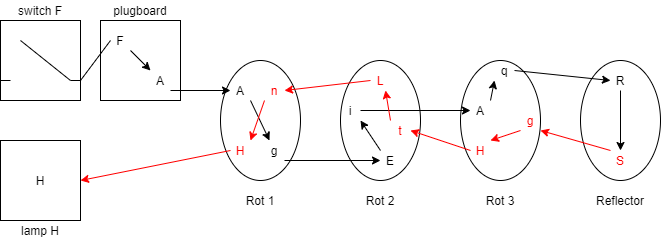
\includegraphics[width = 350pt]{Enigma.png}
\end{figure}

Per costruzione una lettera non è mai cifrata con se stessa. Questa proprietà e quella di riflessione sono state utilissime nel rompere questo sistema.

I rotori non sono fissi, per ogni lettera battuta il primo fa uno scatto, dopo 26 battute il secondo rotore fa uno scatto, dopo $26 \cdot 26$ battute fa uno scatto il terzo rotore. Ad ogni passo quindi la configurazione cambia.

Le permutazioni sono 26 per il primo rotore rispetto al secondo, 26 del secondo rispetto al terzo, 26 del terzo rispetto al riflettore: $26 \cdot 26 \cdot 26 = 17'576$ chiavi se i rotori sono immutabili e noti a chiunque ne avesse una copia. Si aumentano quindi le chiavi scambiando l'ordine dei rotori, quindi si sale a $2^6 \cdot 3! > 10^5$.

Aggiungendo le plugboard si possono scambiare 6 coppie di caratteri per ogni trasmissione, si arriva quindi ad una sequenza di 12 caratteri per descrivere il cablaggio: le combinazioni possibili sono $\binom{26}{12} \approx 10^7$. Scelte le lettere va scelta la loro ordinazione: $12!$, in realtà meno perché molte permutazioni lasciano lo stesso effetto: AB CD = CD AB, ma anche AB = BA, quindi le $6!$ disposizioni delle coppie sono uguali, si ottiene quindi $\binom{26}{12} \cdot \frac{12!}{6! \cdot 2^6} > 10^11$ (10 milioni di miliardi)

Un conteggio alternativo sarebbe: si scelgono 6 coppie di variabili in :
$$ \binom{26}{2} \binom{24}{2} \binom{22}{2} \binom{20}{2} \binom{18}{2} \binom{16}{2} = \frac{26!}{2^6 \cdot 6!} = \binom{26}{12} \cdot \frac{12!}{2^6} $$
dividiamo per le $6!$ permutazioni delle coppie:
$$ \binom{26}{12} \cdot \frac{12!}{2^6 \cdot 6!} $$

La macchina Enigma usata durante la $2^{a}$ guerra mondiale forniva invece 8 rotori in dotazione tra i quali sceglierne 3 e le coppie da scambiare nella plugboard divennero 10.

Ogni reparto disponeva di un libro con l'elenco delle chiavi: assetto dei rotori, quali rotori, in quale ordine e quali coppie connettere con la plugboard. Con l'assetto iniziale si trasmetteva la nuova chiave del messaggio indicante l'assetto per quella trasmissione. La difficoltà stava nella velocità necessaria in quanto il sistema cambiava continuamente. Portò alla creazione di COLOSSUS (1944) che fu un prototipo embrionale dei successivi calcolatori elettronici.
\section{Cifrari perfetti}
Sono cifrari che offrono una sicurezza incondizionata, con certezza assoluta di fronte a qualsiasi potenza di calcolo.
Con un sistema perfetto anche un attacco a forza bruta non può romperlo.

Si paga un caro prezzo nella loro implementazione, infatti si usano solo per pochi ambiti,
per la crittografia comune si preferisce avere una sicurezza computazionale scommettendo su $P \neq NP$.

Questo concetto è stato formalizzato da Shannon (nel 1949) informalmente un
cifrario è perfetto se la sicurezza è garantita qualunque sia l'informazione carpita dal canale.
Abbiamo lo spazio dei messaggi $MSG$ e lo spazio dei crittogrammi $CRITTO$.

Abbiamo poi le variabili aleatorie $M \in MSG$ che descrive il comportamento del mittente e $C \in CRITTO$ che descrive il processo di comunicazione sul canale.

\begin{itemize}
    \item P(M=m) : probabilità che il mittente voglia spedire il messaggio m
    \item P(M=m $ \mid $ C=c) : probabilità condizionata (a posteriori) che il messaggio inviato sia m posto che sul canale transita $C \in CRITTO$
\end{itemize}

Si suppone che il crittoanalista conosca tutto il sistema tranne la chiave. Conosce:
\begin{itemize}
    \item distribuzione di probabilità con cui il mittente invia un messaggio
    \item conosce il cifrario
    \item conosce lo spazio delle chiavi K
\end{itemize}

\emph{Un cifrario è perfetto se $\forall m \in MSG$, $\forall c \in CRITTO$ vale:}
$$ P(M=m  \mid  C=c) = P(M=m) $$

Cioè: la conoscenza di C non ci permette di inferire nulla sul messaggio.

Es: supponiamo: 
$$P(M=\bar{m}) = p > 0, 0 < p < 1$$
$$\exists \bar{m}, \bar{c} : P(M=\bar{m} \mid C=\bar{c}) = 1$$
si ha quindi che se sul canale passa $\bar{c}$ il messaggio è sicuramente $\bar{m}$ quindi aumenta la nostra conoscenza sul sistema. Questo sistema non è perfetto!

Es: supponiamo:
$$\exists \bar{c} : P(M=\bar{m} \mid C=\bar{c}) = 0$$
ci permette di dire che se passa $\bar{c}$ non è stato spedito il messaggio m, anche qui la nostra conoscenza aumenta. Questo sistema non è perfetto!

In un cifrario perfetto la conoscenza complessiva del crittoanalista non cambia dopo che è stato osservato un crittogramma in transito: m e c sono del tutto scorrelati, c appare essere una sequenza casuale.

\subsection{Th di Shannon}
\emph{In un cifrario perfetto il numero delle chiavi deve essere maggiore o uguale al numero dei messaggi possibili}
\subsubsection{Dimostrazione}
$$N_m = \#\{m \in MSG : P(M=m)>0\}$$
$$N_k = \#\{\text{insieme delle chiavi}\}$$
Supponiamo per assurdo che $N_k < N_m$, presi quindi gli spazi si ha questa situazione:

\begin{figure}[H]
  \centering
  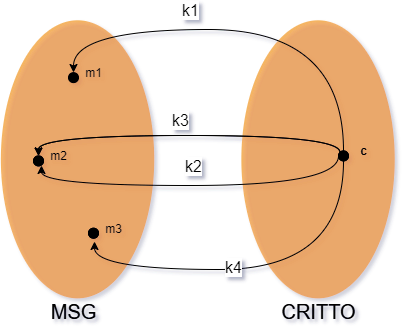
\includegraphics[width = 250pt]{Shannon_proof.png}
\end{figure}

Per i crittogrammi $c : P(C=c) > 0$ possono corrispondere $s$ messaggi, cioè tutti i messaggi che ottengo decriptando $c$ con tutte le chiavi possibili. Si ha necessariamente che $S \leq N_k$ supponendo che chiavi diverse vadano in messaggi diversi si ottiene $S = N_k$ ma magari più chiavi decifrano il messaggio allo stesso modo quindi $S < N_k$. In generale sarà vero che $S \leq N_k$ quindi unendo:
$$ S \leq N_k < N_m \xrightarrow{} S < N_m $$
quindi il numero dei messaggi che possono corrispondere a c è $<$ dei messaggi possibili, quindi deve esistere un $m \in MSG$, $P(M=m) > 0$ tale che:
$$ P(M=m \mid C=c) = 0 $$
(decifrando $c$ esisterà un $m$ che sicuramente non è il messaggio) inferisco della conoscenza, quindi contraddico il cifrario perfetto.

Ne deriva quindi che $N_m \leq N_k$. Per usare un cifrario perfetto mi serve quindi una chiave lunghissima!

\subsection{One-Time Pad}
E' un cifrario precedente Shannon, è simile ad un Vigenère con chiave lunga quanto il messaggio ma su un alfabeto binario. Nasce nel 1917 da Mauborge Vernam. Come alfabeto si usa \{0, 1\}, MSG, CRITTO, KEY sono spazi delle sequenze binarie e l'algoritmo di cifratura è noto a tutti ed è lo XOR (somma modulo 2):

Supponiamo quindi $m, k \in \{0, 1\}^{n}, n > 0$:
$$ c = C(m, k) = m \oplus k $$
$$ m = D(c, k) = c \oplus k$$

Infatti: $m = c \oplus k = m \oplus k \oplus k = m \oplus 0 = m$

NB: \emph{la chiave deve essere NON riutilizzabile}, se così non fosse si avrebbero problemi:
$$ c_1 = m_1 \oplus k $$
$$ c_2 = m_2 \oplus k $$
$$ c_1 \oplus c_2 = m_1 \oplus k \oplus m_2 \oplus k = m_1 \oplus m_2 $$
non ottengo la chiave, ma se ottengo degli zeri in alcune posizioni, so che lì i due messaggi in chiari sono uguali, quindi ottengo conoscenza sulla chiave/messaggio.

NB: l'unica informazione ottenibile dal one-time-pad è la lunghezza del messaggio

\subsubsection{Teorema sul one-time pad}
Se:
\begin{itemize}
    \item tutti i messaggi hanno lunghezza $n$, se più corti li paddo, se più lunghi li divido in blocchi
    \item tutte le sequenze di $n$ bit hanno probabilità maggiore di zero di essere inviate (tutte le sequenze di bit sono messaggi)
    \item usare una chiave scelta perfettamente a caso per ogni messaggio
\end{itemize}
allora: \emph{one-time pad è perfetto e minimale} (usa un numero minimo di chiavi)

\subsubsection{Dimostrazione perfettezza}
$$ \forall m \in MSG, \forall c \in CRITTO $$
$$ P(M=m \mid C=c) = P(M=m) $$

Si ricordi che:
$$ P(M=m \mid C=c) \triangleq \frac{P(M=m\text{ e }C=c)}{P(C=c)} $$
stimiamo il numeratore: per le proprietà dello XOR fissato $m$ esiste una sola chiave che mi produce $c$ perché chiavi diverse producono crittogrammi diversi:
$$ \exists! k \in KEY: m \oplus k = c $$
quindi la probabilità di ottenere $c$ da $m$ è pari alla probabilità di scegliere casualmente $k$: $\frac{1}{2^n}$
quindi $\forall c \in CRITTO$ $P(C=c)=\frac{1}{2^n}$
nessuna dipendenza dal messaggio quindi sono eventi indipendenti: \{M=m\}, \{C=c\} indipendenti, quindi:
$$ P(C=c\text{ e }M=m) = P(M=m) \cdot P(C=c) $$
tornando alla definizione di perfetto possiamo sostituire:
$$
    P(M=m \mid C=c) = \frac{P(M=m\text{ e }C=c)}{P(C=c)} = \frac{P(M=m) \cdot \cancel{P(C=c)}}{\cancel{P(C=c)}}
$$
siamo arrivati alla definizione di perfetto!

\subsubsection{Dimostrazione minimale}
Da Shannon vale che $N_k \geq N_m$ ma nel one-time pad su lunghezza
$n$ ho $N_k = N_m= N_{CRITTO} = 2^n$.
Anche le chiavi sono sequenze di bit e ne uso il numero minore possibile.

\subsubsection{Osservazioni}
Rimuoviamo l'ipotesi che tutte le sequenze di $n$ bit siano messaggi possibili:
in inglese i messaggi significativi sono solo $\alpha^{n}$ con $\alpha = 1.1 \xrightarrow{} \alpha^n << 2^n$.

Proviamo quindi a ridurre la grandezza della chiave:
$N_m = \alpha^n$ dato che $N_k \geq N_m = \alpha^n$.

La chiave sarà una sequenza di $t$ bit tale che:
$$ t: 2^t \geq \alpha^n \xrightarrow{} t \geq log_2\alpha^n = n \cdot log_2\alpha \xrightarrow{} t \geq 0.12 \cdot n$$
Posso quindi usare chiavi molto più corte: $\approx 10\%$ di $n$.

Come fare? Genero i $t$ bit randomicamente e li estendo in maniera deterministica su $n$ bit.
Dobbiamo però metterci al riparo dall'attacco forza bruta: è fondamentale che coppie diverse di
$(m, k)$ producano lo stesso crittogramma. Per far ciò il $\#(m, k)$ deve essere di molto maggiore di $\#CRITTO$:
$$ \alpha^n \cdot 2^t >> 2^n \xrightarrow{} t >> 0.88n$$
In definitiva ci serve $t >> 88\%n$ quindi non si ha una grande compressione della chiave.
\section{DES}
Il \emph{Data Encryption Standard} è un cifrario simmetrico che è stato lo standard per la crittografia di massa fino all'avvento dell'AES.
E' infatti il primo algoritmo che si basa sui principi di Shannon.
\begin{itemize}
    \item \emph{diffusione}: ogni carattere del cifrato dipende da tutti i caratteri del testo in chiaro
    \item \emph{confusione}: combinare testo in chiaro e chiave in modo complesso in modo che osservare il crittogramma non possa portare a separare le due sequenze
\end{itemize}
Questi principi sono importantissimi per la resistenza agli attacchi di crittoanalisi statistica.

Nasce nel 1972 quanto NBS (National Bureau of Standard) ora NIST (National Institute for Security and Technology) chiese la creazione di un algoritmo di crittografia simmetrica in modo da crearne uno standard. In particolare le richieste erano:
\begin{itemize}
    \item sicurezza basata sulla segretezza della chiave e non sul processo di cifratura e decifrazione (dovevano essere pubblici)
    \item l'algoritmo doveva essere efficiente sia in software che in hardware
    \item la sua sicurezza doveva essere certificata da terzi
\end{itemize}
Alla seconda richiesta l'IBM propose \emph{Lucifer} e lo lasciò studiare alla NSA che introdusse alcune variazioni:
\begin{itemize}
    \item la chiave da 128 bit passa a 56 bit
    \item cambia la S-box utilizzata
\end{itemize}

Finalmente nel 1977 viene accettato e reso pubblicamente disponibile (licenza d'uso gratuito). Diventa uno standard.
E' rimasto in vita fino al 1999 quando ne è stato sconsigliato l'uso per una versione più aggiornata: il 3-DES.
Nel 2005 anche il 3-DES diventa sconsigliato a fronte dell'AES proposto nel 2000 ed entrato nel 2001 all'utilizzo di massa.

Nel DES la cifratura è a blocchi di 64 bit, la chiave è di 64 bit in cui 56 sono casuali ed 8 sono di parità (ogni 7 un bit di parità).
La cifratura si compone di $r=16$ fasi in cui si ripetono le stesse operazioni. In ogni fase si sceglie una chiave detta sottochiave di fase.

\begin{wrapfigure}[28]{L}{4.75cm}
    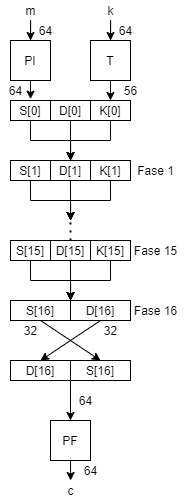
\includegraphics[width = 125pt]{DES_1.png}
\end{wrapfigure} 
I componenti sono:
\begin{itemize}
    \item m: blocco del messaggio
    \item c: corrispondente blocco del crittogramma
    \item k: chiave segreta con i bit di parità
    \item PI: permutazione iniziale (non c'è sempre)
    \item PF: permutazione finale (non c'è sempre)
\end{itemize}
Il messaggio si divide in due parti: S, D ed entrano assieme alla chiave nelle varia fasi, si esegue questo per 16 volte, alla fine si permuta se c'è bisogno e si è ottenuto il blocco.

Per decifrare si esegue lo stesso procedimento ma con le chiavi al contrario. Per ogni $i=1, 2, \_, 16$ abbiamo:
$$ S[i-1], D[i-1], K[i-1] $$
e si applicano:
$$ S[i] = D[i-1] $$
$$ D[i] = S[i-1] \oplus f(D[i-1],K[i-1]) $$

La funzione usata è \emph{non} lineare ed è detta \emph{S-box}. PI, PF e T sono delle tabella che vanno lette per riga:
\begin{itemize}
    \item PI riordina i bit di $m=m_1m_2\_m_64$ come $m_{58}m_{50}\_m_{7}$ (bit 1 va in posizione 40, il bit 58 va in posizione 1, ecc, ecc)
    \item PF è la permutazione inversa di PI (quindi riporta il bit 40 in posizione 1, ecc, ecc)
    \item T scarta i bit di parità ($k_8, k_{16}, \_, k_{64}$) e questa sequenza di 56 bit costituisce, dopo una permutazione, la chiave K[0].
\end{itemize}

La fase $i$-esima del DES è:

\begin{figure}[H]
    \centering
    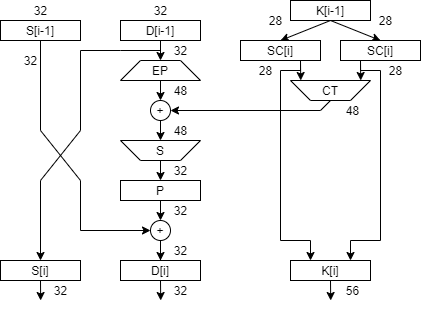
\includegraphics[width = 300pt]{DES_2.png}
\end{figure}
con:
\begin{itemize}
    \item SC: shift ciclico a sx di:
    \begin{itemize}
        \item 1 se $i \in \{1, 2, 9, 16\}$
        \item 2 altrimenti
    \end{itemize}
    \item P: permutazione
    \item EP: espansione
    \item S: S-box
    \item CT: elimina alcuni bit della chiave e li permuta
\end{itemize}

\begin{wrapfigure}{l}{4cm}
    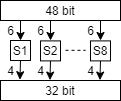
\includegraphics[width = 100pt]{DES_3.png}
\end{wrapfigure}
La S-box ha questa struttura:
Implementa 8 funzioni booleane a 6 input e a 4 output (in bit).
Si costruisce tramite la tabella di verità delle singole funzioni.

\clearpage

Queste tabelle di verità vanno però lette in una maniera particolare (di seguito la tabella di S1):
\begin{table}[ht!]
    \centering
    \small
    \begin{tabular}{c|c c c c c c c c c c c c c c c c}
        & 0 & 1 & 2 & 3 & 4 & 5 & 6 & 7 & 8 & 9 & 10 & 11 & 12 & 13 & 14 & 15 \\
        \hline
        0 & 14 & 4 & 13 & 1 & 2 & 15 & 11 & 8 & 3 & 10 & 6 & 12 & 5 & 9 & 0 & 7 \\
        1 & 0 & 15 & 7 & 4 & 14 & 2 & 13 & 1 & 10 & 6 & 12 & 11 & 9 & 5 & 3 & 8 \\
        2 & 4 & 1 & 14 & 8 & 13 & 6 & 2 & 11 & 15 & 12 & 9 & 7 & 3 & 10 & 5 & 0 \\
        3 & 15 & 12 & 8 & 2 & 4 & 9 & 1 & 7 & 5 & 11 & 3 & 14 & 10 & 0 & 6 & 13 \\
    \end{tabular}
\end{table}
supponiamo di avere 010011: prendo gli estremi 0 ed 1 ed uso quasto come indice per la riga, prendo poi i 4 bit centrali (1001) e lo uso come indice di colonna. Accedo quindi a (1, 9) $\xrightarrow{} 06$.

NB: perché è importante che non sia lineare? Perché $f(x \oplus y) \neq f(x) \oplus f(y)$ ed è cruciale ai fini del funzionamento!

\subsection{Vulnerabilità}
Siano:
$$ c = C_{DES}(m, k) $$
$$ c^{*} = C_{DES}(m', k') $$
$$ m', k' \text{ complementari di m e k} $$

Si può notare che $c^{*} = c$ perché SC sposta i bit complementati quindi EP espande bit complementati e poi c'è lo XOR che ci da un risultato uguale a quello che avremmo se non fossero complementate:
$$ \bar{m_i} \oplus \bar{K_i} = (1 \oplus m_i) \oplus (1 \oplus K_i) = m_i \oplus K_i $$
L'input alla S-box è identico! Abbiamo quindi in uscita lo stesso valore che poi verrà messo in XOR con l'altra parte del messaggio che è complementato, ci fornisce quindi il risultato complementato.

\subsection{Attacchi al DES}
Sono tutti attacchi a forza bruta:
\begin{itemize}
    \item architetture appositamente progettate per attaccare il DES e quindi velocizzare criptazione e decriptazione (con 1M\$ si costruiva una macchina che forzava il DES in 35 minuti)
    \item distribuire lo spazio delle chiavi tra più utenti, è più economico e la velocità dipende da quanti utenti ci lavorano
\end{itemize}

Nel 1997 la compagnia RSA lancia una sfida: in 5 mesi esplorando il 25\% delle chiavi viene risolta la sfida e trovata la chiave.
Nel 1998 ce ne vollero 39 di giorni esplorando 85\% delle chiavi.

Qualche parola su questi attacchi: le chiavi possibili sono $2^{56}$, 64 di queste chiavi sono rimosse perché con regolarità. Ricordando che:
$$ C(m, k) = c = \bar{c} = C(\bar{m}, \bar{k}) $$
si possono dimezzare le chiavi passando a $2^{55}$ (55 bit di sicurezza). Questo è un tipo di attacco chosen plain-text in cui ci si procura delle coppie $<m, c_1>$, $<\bar{m}, c_2>$. Si inizia ad esplorare le chiavi e per ognuna si controlla:
\begin{itemize}
    \item C(m, k) = $c_1$: k POTREBBE ESSERE la chiave
    \item C(m, k) = $c_2$: $\bar{k}$ POTREBBE essere la chiave
    
    NB: $C(m,k) = \bar{c_2} \iff C(\bar{m},\bar{k}) = \bar{\bar{c_2}} = c_2$ in quanto sappiamo che $C(m, k) = c$ e $C(\bar{m}, \bar{k})=\bar{c}$. Escludo quindi due chiavi alla volta.
    \item $\neq c_1, \bar{c_2}$: si prova un'altra chiave (k e $\bar{k}$ non lo sono)
\end{itemize}

Nel 1990 sono stati scoperti attacchi di \emph{crittoanalisi differenziale} (da Bihan e Shamir). E' un attacco di tipo chosen plain-text in cui ci si procura $2^{47}$ coppie $<m,c>$.
Si cerca tra i messaggi simili le similitudini nei crittogrammi e si sfruttano per trovare la chiave.
Si assegnano delle probabilità alle singole chiavi, ed emerge poi quella più probabile.
Dato che le fasi sono 16 si ha un costo di questo attacco pari a $2^{55.1}$, poco più di una ricerca esaustiva.

NB: se fosse $r=8$ si avrebbe difficoltà $2^{14}$

Nel 1993 sono stati scoperti attacchi di \emph{crittoanalisi lineare} che consistono nella costruzione di una approssimazione lineare della S-box che ci permette di inferire taluni bit della chiave, il resto si bruta.
Si scende a $2^{43}$ coppie $<m, c>$ ed è di tipo known plain-text.
Metodo più efficiente del forza bruta.

\subsection{Varianti del DES}

\subsubsection{Scelta indipendente delle sottochiavi}
Anziché generare le sottochiavi di fase a partire dalla chiave principale si scelgono manualmente.
E' come passare da 56 bit a $16 \cdot 48 = 768$ bit di chiave.
Tuttavia non porta effettivamente ad un aumento della sicurezza perché è sempre vulnerabile ad attacchi differenziali portando a $2^{61}$ la complessità di un attacco.

\subsubsection{Cifratura multipla: 2DES}
$$ \forall k_1, k_2, k_3: C_D(C_D(m, k_1), k_2) \neq C_D(m, k_3) $$
quindi applicare due volte la cifratura DES non è uguale ad applicarlo una sola volta.
Si arriva ad uno spazio delle chiavi di $2^{112}$.
Tuttavia esiste l'attacco \emph{meet-in-the-middle} che fa scendere la sicurezza a 57 bit di chiave:
$$ c = C(C(m,k_1), k_2) $$
$$ D(c,k_2) = C(m,k_1) $$
possiamo quindi prendere una coppia $<m, c>$:
$$ \forall k_1 \text{ mi salvo } C(m, k_1) \xrightarrow{} 2^{56} \text{ cifrature }$$
$$ \forall k_2 \text{ mi calcolo } D(c, k_2) \xrightarrow{} 2^{56} \text{ cifrature al più }$$
Cercando nella lista delle cifrature, so che esisterà una coppia $<k_1, k_2>$ per la quale c'è la corrispondenza:
$$ D(c, \bar{k_2}) = C(m, \bar{k_1}) $$.

Questo attacco costa quindi $2^{56} + 2^{56} = 2 \cdot 2^{56} = 2^{57}$ al più, tra cifrature e decifrature.

\subsubsection{Cifratura multipla: 3DES}
Presente in due modi:
\begin{itemize}
    \item 2TDEA:
        $$ c = C(D(C(m, k_1), k_2), k_1) $$
        $k_1$ e $k_2$ sono chiavi di 56 bit tra di loro indipendenti. Si sceglie questa modalità perché se pongo $k_1 = k_2$ ottengo il DES normale, quindi risulta essere retrocompatibile.
        
        NB: CDC non è più robusto di CCC. Ha un livello di sicurezza di 112 bit.
    \item 3TDEA: triple data encryption algorithm
        $$ c = C(D(C(m, k_1), k_2), k_3) $$
        $k_1$, $k_2$, $k_3$ chiavi a 56 bit. Si hanno quindi chiavi di $3 \cdot 56 = 168$ bit. E' vulnerabile a meet-in-the-middle quindi la sicurezza scende a 112 bit di sicurezza.
\end{itemize}
\section{AES}
Nel 1998 esce il bando per ricercare un nuovo algoritmo per soppiantare il DES ed il 3DES.
Ci furono 21 proposte che dovevano tenere conto di
\begin{itemize}
    \item sicurezza: resistere a tutti gli attacchi noti
    \item costo di realizzazione: doveva essere facile implementarlo sia in software che in hardware
    \item caratteristiche algoritmiche: portabile su diverse macchine, usabile con chiavi di diversa lunghezza
    \item libero da brevetti in quanto il nuovo standard doveva divenire libero da utilizzare
\end{itemize}

Nell'Ottobre del 2000 si sceglie l'AES e nel 2001 diventa lo standard.
E' un algoritmo che ancora oggi continua a conservare tutti i bit di sicurezza.
Gli altri 4 cifrari arrivati alla fine erano:
\begin{itemize}
    \item MARS (IBM)
    \item RCG (RSA)
    \item Rijndael (Proton word int + Università di Leuven, Belgio)
    \item SERPENT (Università di Israele, UK, USA)
    \item TWOFISH (Berkeley, Princeton)
\end{itemize}
Rijndael vince il bando e diventa AES con qualche modifica.

Permette chiavi di 128, 192, 256 bit, ma noi vedremo la versione a 128 bit.
Si usa su blocchi anch'essi di 128 bit. Funziona per fasi:
\begin{itemize}
    \item 10 fasi $\xrightarrow{}$ 128 bit
    \item 12 fasi $\xrightarrow{}$ 192 bit
    \item 14 fasi $\xrightarrow{}$ 256 bit
\end{itemize}

\subsection{Selezione delle sottochiavi di fase}
Si parte da 128 bit di chiave posizionati in una matrice $4 \times 4$ byte per colonna:

$$
K = 
    \begin{bmatrix}
        K[0] & K[4] & K[8] & K[12] \\
        K[1] & K[5] & K[9] & K[13] \\
        K[2] & K[6] & K[10] & K[14] \\
        K[3] & K[7] & K[11] & K[15]
    \end{bmatrix}
$$

Prese le colonne in ordine da sinistra verso destra abbiamo: 
$$W(0), W(1), W(2), W(3)$$
Costruiamo quindi $W(i)$ che è una sequenza di byte che usiamo per generale le sottochiavi di fase.
Per ogni $t \geq 4$:
\begin{equation}
    W(t) = 
    \begin{cases}
        W(t-1) \oplus W(t-4) \text{ se t non è multiplo di 4} \\
        T(W(t-1)) \oplus W(t-4) \text{ se t è multiplo di 4}
    \end{cases}
\end{equation}

T è una funzione non lineare applicata tramite una S-box.
La chiave dell'$i$-esima fase è quindi composta da:
$W(4 \cdot i), W(4 \cdot i + 1), W(4 \cdot i + 2), W(4 \cdot i + 3),$

\subsection{Preparazione}
La cifratura si fa per blocchi (di 128 bit in questo caso).
Si creano i blocchi caricandoli \emph{per colonna} in una matrice $4 \times 4$ byte:
$$
B = 
    \begin{bmatrix}
        b_{00} & b_{01} & b_{02} & b_{03} \\
        b_{10} & b_{11} & b_{12} & b_{13} \\
        b_{20} & b_{21} & b_{22} & b_{23} \\
        b_{30} & b_{31} & b_{32} & b_{33}
    \end{bmatrix}
    b_{ij} \in \{0, 1\}^{8}
$$

Si applica una prima trasformazione applicando la chiave:
$$ B \oplus K $$

\subsection{Fasi}
Dopodiché si inizia con le fasi, ognuna di esse composta da 4 operazioni:
\begin{itemize}
    \item \emph{substitution bytes}
    \item \emph{shift rows}
    \item \emph{mix columns}
    \item \emph{add round key}
\end{itemize}
Le prime 3 operazioni applicano: non linearità, diffusione e confusione.
L'ultima fase aggiunge la chiave.

Nell'ultima fase \emph{non} si applica la mix columns. Alla fine delle iterazioni si ottiene il crittogramma.
La S-Box dell'AES è sempre usata in forma di tabella di verità, ma a differenza di quella del DES si conosce la funzione che la genera!

\subsection{Substitution bytes}
Ogni byte viene trasformato usando la S-Box:
$$ b_{ij} \xrightarrow{} S-Box(b_{ij}) $$

Questa S-Box si compone di una matrice $16 \times 16$ di interi $\in [0, 255]$ e contiene una permutazione dei numeri di questo intervallo.
L'accesso alla S-Box viene fatto suddividendo il byte $b_{ij}$ in due blocchi da 4 bit l'uno:
$$ b_{ij} = b_{1}b_{2}b_{3}b_{4} \mid b_{5}b_{6}b_{7}b_{8} $$
i primi 4 bit formano il numero di \emph{riga}, gli ultimi 4 bit formano il numero di colonna.

La relazione implementata dalla S-Box è:
$$ x \xrightarrow{} x^{-1} + c $$
questo inverso è l'inverso moltiplicativo in $GF(2^{8})$ con l'aggiunta di una componente lineare.
In questo insieme la somma viene eseguita tramite lo XOR (somma modulo 8), mentre la moltiplicazione è eseguita $\mod 2^{8}$.
Nella pratica ogni byte può essere visto come un polinomio, facendo la moltiplicazione si fa il prodotto tra polinomi ma in modulo, quindi si tagliano via i gradi oltre al settimo.
NB: GF: Galois Field - campi finiti di Galois

Questa S-Box ha una bassissima correlazione tra i bit di ingresso e di uscita.
Inoltre essendo usata sia per la chiave che per la matrice del messaggio si ha una maggiore sicurezza

\subsection{Shift rows}
Si usa per spargere il messaggio.
Lascia invariata la prima riga, shifta a sx di 1, 2, 3 le altre righe, rispettivamente.

$$
    \begin{bmatrix}
        b_{00} & b_{01} & b_{02} & b_{03} \\
        b_{10} & b_{11} & b_{12} & b_{13} \\
        b_{20} & b_{21} & b_{22} & b_{23} \\
        b_{30} & b_{31} & b_{32} & b_{33}
    \end{bmatrix}
\xrightarrow{}
    \begin{bmatrix}
        b_{00} & b_{01} & b_{02} & b_{03} \\
        b_{11} & b_{12} & b_{13} & b_{10} \\
        b_{22} & b_{23} & b_{20} & b_{21} \\
        b_{33} & b_{30} & b_{31} & b_{32}
    \end{bmatrix}
$$
Ho quindi diffuso i byte di ogni colonna su tutte le altre.

\subsection{Mix columns}
Si mixano le colonne attraverso una moltiplicazione per matrice.
M matrice $4 \times 4$ byte, per ogni colonna:
$$
    B_{j} \xrightarrow{} M \cdot B_{j}
$$
Anche qui si lavora in GF($2^8$). Questo porta ogni elemento della colonna ad essere dipendente da tutti i byte della colonna.

\subsection{Add round key}
$$
    b_{ij} \xrightarrow{} b_{ij} \oplus K_{ij} \text{ chiave della sottofase}
$$
NB: si noti che shift rows e mix columns arrivano alla massima diffusione già al secondo round in quanto ogni byte è dipendente da tutti gli altri del messaggio.

NB: i 128 bit sono tutti bit di sicurezza ancora oggi!

Esistono attacchi che rendono vulnerabile il cifrario se usato con 6 round, lo standard tuttavia ne vuole 10 quindi fino ad ora non abbiamo nessun problema.

E' vulnerabile ad attacchi di tipo \emph{side-channel} ma questi attacchi sono indipendenti dal sistema.

\subsection{Cifratura a blocchi}
Sia il DES che l'AES cifrano il plaintext a blocchi, AES ad esempio divide in blocchi grandi quanto la chiave e poi si cripta.
Il problema di ciò è che blocchi uguali vengono cifrati in blocchi uguali, questo può dare molte informazioni.
Per risolvere questo problema si cerca di inserire una dipendenza tra il blocco $i$-esimo e quelli che vengono prima.
Nell'AES si prende $m$ e lo si divide in blocchi da 128 bit:
$$ m = m_{1}m_{2}\_m_{i}\_m_{e} $$
\begin{itemize}
    \item se $\mid m_e \mid < 128$ allora si aggiunge $10...0$ fino ad arrivare a 128
    \item se invece $ \mid m_e \mid = 128 $ si inserisce un intero blocco $10...0$ in modo da avere sempre questo terminatore.
\end{itemize}
Successivamente si sceglie una $c_0$ random che può anche essere trasmessa in chiaro e si attua questo schema:
\begin{figure}[H]
    \centering
    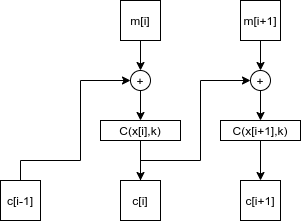
\includegraphics[width = 200pt]{CBC.png}
\end{figure}

$$
    x_{i} = m_{i} \oplus c_{i-1}
$$
$$
    c_{i} = C(m_{i} \oplus c_{i-1}, K)
$$
questa modalità è detta \emph{CBC: Cipher Block Chaining}.
La decifrazione invece si esegue in questo modo:
\begin{figure}[H]
    \centering
    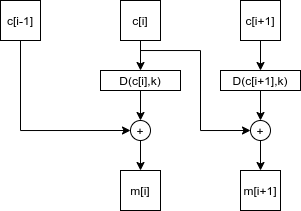
\includegraphics[width = 200pt]{CBC_2.png}
\end{figure}

$$
    m_i = D(c_i, K) \oplus c_{i-1}
$$

NB: mentre la cifratura va eseguita necessariamente sequenzialmente la decifratura si può eseguire in parallelo.
Inoltre se invio il testo cifrato e ci sono errori risolta in un errata decifrazione solo del blocco $i$ e $i+1$ mentre gli altri continuano ad essere decriptati correttamente.

\subsection{Altri cifrari simmetrici}
\begin{itemize}
    \item \emph{Ron's Code 5} (RC5): simile al DES, ma migliorato.
    Blocchi da 64 bit e chiavi di $c \cdot 32$ bit, $r$ fasi (consigliate 16). $r$ e $c$ scelti a piacere. Usa shift ciclico, XOR, addizione $\mod 2^{32}$. Semplice da realizzare e sicuro
    \item \emph{International Data Encryption Algorithm} (IDEA): chiave a 128 bit, usa shift ciclico, XOR, moltiplicazione $\mod (2^{16} + 1)$ ed addizione $\mod 2^{16}$. Più semplice e sicuro del DES
\end{itemize}
\section{Crittografia a chiave pubblica}
Ricorcdando il one-time-pad il suo più grande problema risulta essere la lunga chiave, che va scambiata e ricreata ogni volta.
Anche AES necessita di scambio di chiavi.
\emph{Come si può scambiare una chiave in maniera sicura?}
Nel 1976 Diffie ed Hellman con il loro articolo \emph{New Directions in Cryptography} hanno rivoluzionato la crittografia.
Il protocollo \emph{DH} permette la negoziazione di una chiave di sessione senza che le due parti si siano scambiate informazioni in precedenza.
In parallelo sempre gli stessi Diffie ed Hellman propongonono lo schema di crittografia a chiave pubblica, senza tuttavia averne una valida implementazione.
In questo nuovo schema si hanno due chiavi:
\begin{itemize}
    \item una \emph{pubblica} nota a tutti ed utilizzata per cifrare
    \item una \emph{privata} nota solo al ricevente usata per decifrare
\end{itemize}
Ogni utente avrà quindi una coppia
$$ <K_{priv}, K_{pub}> $$

NB: su $n$ utenti ci saranno quindi $n$ coppie di chiavi contro le $n^2$ chiavi nel caso di algoritmi simmetrici

La cifratura ha la forma:
$$ c = C(m, K_{pub}) $$
mentre la decifrazione ha la forma:
$$ m = D(c, K_{priv})$$

NB: si dice asimmetrica perché le due parti fanno cose diverse, non c'è una simmetria.

Questi cifrari devono avere alcune caratteristice:
\begin{itemize}
    \item $D(C(m, K_{pub}), K_{priv}) = m$
    \item efficienza e sicurezza: le chiavi devono essere \emph{facili} da generare e praticamente deve essere impossibile generare la stessa coppia.
    Ciò che è legale deve essere fatto in tempo polinomiale, mentre deve essere difficile ottenere il messaggio conoscendo $c$ e $K_{pub}$
\end{itemize}

Questi requisiti si hanno se si usano le \emph{funzioni one-way trap-door}, funzioni facili da calcolare ma difficili da invertire senza avere maggiori informazioni.

Nel 1977 Rivest, Shamir ed Adleman scoprono una funzione di questo tipo basata sui numeri primi.
L'algoritmo RSA si basa sul fatto che dati $p$ e $q$ primi, calcolare $n = p \cdot q$ è facile, dato $n$ invece è difficile trovate $p$ e $q$.
Inoltre lavora in algebra modulare!

\subsection{Algebra modulare}
E' fondamentale in crittografia in quanto:
\begin{itemize}
    \item riduce lo spazio dei numeri sui quali si opera e rende più veloci i calcoli
    \item rende difficili alcuni problemi computazionalmente semplici (o banali) nell'algebra standard
\end{itemize}

Nell'algebra modulare ad esempio le funzioni tendono ad essere imprevedibili:
\begin{table}[ht!]
    \centering
    \small
    \begin{tabular}{c|c c c c c c c c c c c c}
        $x$ & 1 & 2 & 3 & 4 & 5 & 6 & 7 & 8 & 9 & 10 & 11 & 12  \\
        \hline
        $2^{x}$ & 2 & 4 & 8 & 16 & 32 & 64 & 128 & 256 & 512 & 1024 & 2048 & 4096  \\
        $2^{x} \mod 13$ & 2 & 4 & 8 & 3 & 6 & 12 & 11 & 9 & 5 & 10 & 7 & 1  \\
    \end{tabular}
\end{table}

Mentre nell'algebra normale la funzione esponenziale è monotòna, nell' algebra modulare la funzione è imprevedibile.

Dato $n \in \mathbb{N}$ allora:
$$ Z_{n} = \{ 0, 1, 2, \_, n-1 \} $$
$$ Z_{n}^{*} \subseteq Z_{n} = \{\text{elementi di $Z_{n}$ coprimi con $n$}\} $$


NB: Se $n$ è primo: $Z_{n}^* = \{1, 2, 3, \_, n-1\}$

Dati $a, b \geq 0$ interi e $n > 0$ diremo \emph{a è congruo a b modulo n}:
$$ a \equiv b \mod n $$
se e solo se $\exists k$ intero per cui:
$$ a = b + k \cdot n $$

NB: $a \mod n = b \mod n$, nella relazione di congruenza mod n si riferisce all'intera relazione, nelle relazioni di uguaglianza invece si riferisce solo al membro dove appare:
$$ 5 \neq 8 \mod 3 $$
$$ 2 = 8 \mod 3 $$

\subsubsection{Altre proprietà}
$$ (a+b) \mod m = (a \mod m + b \mod m) \mod m $$
$$ (a-b) \mod m = (a \mod m - b \mod m) \mod m $$
$$ (a \cdot b) \mod m = (a \mod m \cdot b \mod m) \mod m $$
$$ a^{r \times s} \mod m = (a^r \mod m)^{s} \mod m $$

\subsection{Funzione di Eulero}
$$ \phi(n) = \mid Z_{n}^{*} \mid $$
indica il numero di interi minori di $n$ e coprimi con esso.

NB: $n$ primo $\implies$ $\phi(n) = n-1$

Se $n$ è composto
$$ \phi(n) = n \cdot (1 - \frac{1}{p_1}) \cdot \_ \cdot (1 - \frac{1}{p_k})$$
con $p_1$, \_, $p_k$ i fattori primi di n presi senza molteplicità

Se $n = p \cdot q$ con $p$ e $q$ primi (quindi $n$ semiprimo):
$$ phi(n) = (p-1) \cdot (q-1) $$

\subsection{Teorema di Eulero}
$\forall n>1$, $\forall a \in Z_{n}^*$:
$$ a^{\phi(n)} \equiv 1 \mod n $$

\subsection{Piccolo teorema di Fermat}
$\forall n$ primo e $\forall a \in Z_{n}^*$:
$$ a^{n-1} \equiv 1 \mod n $$

NB: $ a^{\phi(n)} \equiv 1 \mod n $ ma essendo $n$ primo $\phi(n) = n-1 \implies  a^{n-1} \equiv 1 \mod n $

\subsection{Conseguenze}
$\forall a \in Z_{n}^*$
$$ a^{\phi(n)} = a \cdot a^{\phi(n)-1} \implies a \cdot a^{\phi(n)-1} \equiv 1 \mod n $$
$$ a \cdot a^{-1} \equiv 1 \mod n $$
$$ a^{-1} = a^{\phi(n)-1} \mod n $$
Quindi $a^{-1} \mod n$ si può calcolare se si conosce $\phi(n)$, quindi se si conoscono $p, q, \_$ primi fattori di $n$.

NB: in generale nell'algebra modulare l'esistenza dell'inverso non è garantita perché $a^{-1}$ deve essere intero.

\subsection{Teorema sull'inverso}
L'equazione $a \cdot x \equiv b \mod n$ ammette soluzioni se e solo se $mcd(a,n)$ divide $b$.
In questo caso si hanno esattamente $mcd(a,n)$ soluzioni distinte.

NB: se $mcd(a,n)=1$ ($a$,$n$ coprimi) $a \cdot x = b \mod n$ ammette una unica soluzione. E quindi esiste $a^{-1}$


\subsection{Algoritmo di Euclide esteso}
Nasce per risolvere l'equazione $a \cdot x + b \cdot y = mcd(a,b)$.
\begin{verbatim}
    Euclide_esteso(a,b):
        se b == 0:
            return (a,1,0)
        _d, _x, _y = Euclide_esteso(b, a mod b)
        d, x, y = _d, _y, _x - (a//b) * _y
        return (d, x, y)
\end{verbatim}
Ha complessità logaritmica nel valore di $a$ e $b$ quindi polinomiale nella dimensione dell'input.

Possiamo usare quest'algoritmo per il calcolo dell'inverso:
$$ ax \equiv 1 \mod n $$
$$ ax = nz + 1 \text{ per un certo valore di z} $$
$$ ax + ny = mcd(a,b) \text{ con y = -z, n = b, 1 = mcd(a,b)} $$
usando l'algoritmo si ottengono $<d, x, y>$, $x$ è proprio il nostro inverso.

\subsection{Generatori}
$a \in Z_{n}^*$ è un \emph{generatore di $Z_{n}^*$} se la funzione:

$$ a^k \mod n \text{ , } 1 \leq k \leq \phi(n) $$

genera \emph{tutti e soli} gli elementi di $Z_{n}^*$.

Un generatore quindi genera $Z_{n}^*$ ma in un ordine difficile da prevedere.

NB: l'unica cosa prevedibile è che $1$ si ottiene solo per $x = \phi(n)$ poiché sappiamo $a^{\phi(n)} = 1 \mod n$ per Eulero. Quindi $\forall g$ $g^k \neq 1 \mod n$, $ 1 \leq k < \phi(n)$

Non tutti gli $n$ forniscono generatori per $Z_{n}^*$.

\subsection{Teorema sui generatori}
Se $n$ è primo allora $Z_{n}^*$ ha almeno un generatore.

Per $n$ primo non tutti gli elementi di $Z_n^*$ sono suoi generatori (1 non lo è mai).

Per $n$ primo i generatori di $Z_n^*$ sono $\phi(n)$.

\subsection{Problemi sui generatori}
Determinare un generatore di $Z_n^*$ con $n$ primo è difficile, si possono provare tuttu i numeri in $[2, n-1]$ ma è esponenziale nella dimensione di $n$.
Esistono tuttavia algoritmi randomizzati che risolvono il problema efficientemente.

\subsection{Logaritmo discreto}
Consiste nel trovare $x$ che risolve:
$$ a^x \equiv b \mod n, \text{n primo} $$
L'equazione ammette soluzioni $\forall b$ se e solo se $a$ è un generatore di $Z_n^*$.
Tuttavia non possiamo sapere in che ordine sono generati i valori di $Z_n^*$ quindi per trovare $x$ giusto dobbiamo iterare tutti i valori (esponenziale nella dimensione dell'input).

NB: su questa complessità si basa DH.

\subsection{Funzioni one-way trap-door}
$$ n = p \cdot q \text{ p, q primi} $$
è facile.

Dato $n$ trovare $p$ e $q$ richiede tempo (sub)esponenziale. Dato $p$ o $q$ invece si fattorizza velocemente: $q = \frac{n}{p}$, ma anche conoscendo $\phi(n)$ si fattorizza velocemente. E' il problema della \emph{fattorizzazione}

$$ y = x^z \mod s \text{ con x, z, s interi} $$
è facile, si può infatti fare in O($\log_2z$).

Se $s$ non è primo calcolare $x = y^{\frac{1}{z}} \mod s$ richiede tempo esponenziale.
L'estrazione di radice con $s$ non primo è quindi difficile! E' il problema della \emph{radice}

$$y = x^z \mod s $$
è facile.

Trovare $z$ tale che $y = x^z mod s$ dati $x, y, s$ è difficile (ha infatti la stessa complessità della fattorizzazione). E' il problema del \emph{logaritmo discreto}.

\subsection{Vantaggi e svantaggi}
Pro:
\begin{itemize}
    \item meno chiavi
    \item non richiedono lo scambio di chiavi
\end{itemize}
Con:
\begin{itemize}
    \item più lenti della cifratura simmetrica
    \item esposizione ad attacchi chosen plain-text
\end{itemize}

Si può infatti criptare un tot di messaggi $m_1, \_, m_h$ e vedere se sul canale passa uno dei vari $c_1, \_, c_h$. Se compare allora sappiamo il messaggio, se non compare allora sappiamo quale messaggio sicuramente non è.

\subsection{Cifrari ibridi}
Si usa un cifrario a chiave pubblica per scambiare le chiavi AES e successivamente si comunica tramite AES che è veloce. L'attacco chosen plain-text è risolto con chiavi random difficilmente prevedibili.

NB: la chiave pubblica va estratta da un certificato digitale per evitare attacchi man-in-the-middle in cui terzi si spacciano per il destinatario.
\section{RSA}
\subsection{Generazione delle chiavi}
Partiamo dalla creazione della coppia di chiavi, spetta al destinatario:
\begin{itemize}
    \item Si scelgono due primi $p$, $q$ molto grandi ($\approx$1000 bit) (adesso si consiglia che $p \cdot q \approx 2048$ bit). Vanno generati in tempo polinomiale.
    \item Si calcolano $n = p \cdot q$ e $\phi(n) = (p-1) \cdot (q-1)$. Anche qui operazioni in tempo polinomiale nella grandezza dell'input.
    \item Si sceglie $e < \phi(n)$ tale che: $MCD(e, \phi(n))=1$
    \item Si calcola $d = e^{-1} \mod \phi(n)$. Anche questo si può calcolare in tempo polinomiale usando Euclide Esteso.
    
    NB: essendo $MCD(e, \phi(n))=1$ esiste unico $e^{-1}$.
\end{itemize}

Alla fine si hanno quindi le due chiavi:
$$ K_{pub} = (e,n) $$
$$ K_{priv} = (d,n) $$

Naturalmente va tenuto segreto anche il resto delle informazioni: $p$, $q$, $\phi(n)$.

\subsection{Cifratura e decifratura}
I messaggi sono sequenze binarie trattate come un intero! Lo indicheremo con $m$ e deve verificare $m < n$ perché non sarebbe decifrabile altrimenti.
Se $m \geq n$ lo dividiamo in blocchi di $b = \lfloor \log_2n \rfloor$ bit e si aggiunge una dipendenza tra un blocco e l'altro.
Solitamente si fissa un limite comune per la dimensione dei blocchi, prevenendo così l'uso di cifrari poco sicuri $m < 2^b < n$.

La cifratura è quindi eseguita:
$$ c = C(m, K_{pub}) = m^{e} \mod n$$

La decifratura è invece eseguita:
$$ m = D(c, K_{priv}) = c^{d} \mod n$$

Si possono eseguire in tempo polinomiale tramite la fast-exp.

\subsection{Dimostrazione della correttezza}
Si vuole dimostrare:
$$ D(C(m, K_{pub}), K_{priv}) = m $$

Possiamo analizzare 3 casi distinti:

\subsubsection{Caso 1}
Se $p$ e $q$ non dividono $m$, cioè se $m$ ed $n$ sono co-primi. In questo caso vale $MCD(m,n)=1$.

Se componiamo le formule per criptare e decriptare otteniamo:
$$ (m^e \mod n)^d \mod n = m^{e \cdot d} \mod n $$
ricordando che $ed \equiv 1 \mod \phi(n)$ applicando la definizione di congruenza in modulo possiamo scrivere: $ed = 1 + r \cdot \phi(n)$ per qualche $r \in \mathbb{N}$.
Possiamo quindi scrivere:

$$ m^{ed} \mod n = m^{1 + r \cdot \phi(n)} \mod n = m \cdot (m^{\phi(n)})^{r} \mod n$$

Essendo $m$ ed $n$ coprimi vale il Teorema di Eulero: $m^{\phi(n)} = 1 \mod n$ quindi:
$$ m \cdot 1^r \mod n = m \mod n = m $$

\subsubsection{Caso 2}
Supponiamo che $m$ sia divisibile per $p$ e non per $q$. Allora sarà vero che:
$$ m^{ed} = m^{ed} - m \equiv 0 \mod p $$

Ricaviamo una relazione simile anche per $q$ applicando la definizione di riduzione in modulo:
$$ m^{ed} \mod q = m^{\phi(n) \cdot r + 1} \mod q $$

Ora ricordiamo la definizione $\phi(n) = (p-1)\cdot(q-1)$ e possiamo riscrivere come:
$$ m^{ed} \mod q = m^{(p-1)\cdot(q-1)\cdot{r} + 1} \mod q = (m^{q-1})^{(p-1)\cdot{r}}\cdot{m} \mod q $$

Applicando il teorema di Eulero anche qui otteniamo:
$$ 1^{(p-1)\cdot{r}}\cdot{m} \mod q = m \mod q$$

Possiamo quindi scrivere:
$$ m^{ed} \equiv m \mod q \implies m^{ed} - m \equiv 0 \mod q $$
Abbiamo quindi ottenuto:
\begin{equation}
    \begin{cases}
    $$ m^{ed} - m \equiv 0 \mod q $$ \\ 
    $$ m^{ed} - m \equiv 0 \mod p $$
    \end{cases}
\end{equation}
che significa che $ m^{ed} -m $ è divisibile sia per $p$ che per $q$ quindi lo sarà anche per $n = p \cdot q$, possiamo quindi dire:
$$ m^{ed} -m \equiv 0 \mod n => m^{ed} \equiv m \mod n = m $$

\subsubsection{Caso 3}
Avere $m$ divisibile sia per $p$ che per $q$ significa che è divisibile per $n$, il che è impossibile in quanto un messaggio, per essere corretto, deve soddisfare $m < n$.

\subsection{Sicurezza ed attacchi}
La sicurezza è legata alla fattorizzazione, se fattorizzo $n$ ho $p$ e $q$ e da li posso trovare $\phi(n)$. Non sappiamo però se è necessaria la fattorizzazione o si potrebbe forzare in altri modi.

Potrebbe essere necessaria perché il problema è quello di calcolare $m = \sqrt[e]{c} \mod n$ ed è difficile quanto fattorizzare $n$.
Calcolare $\phi(n)$ direttamente da $n$ equivale a fattorizzare $n$.
In particolare il calcolo di $\phi(n)$ o la fattorizzazione di $n$ si trasformano l'uno nell'altro in tempo polinomiale: sono computazionalmente equivalenti:

Fattorizzato $n = p \cdot q \xrightarrow{} \phi(n) = (p-1) \cdot (q-1)$

Calcolato $\phi(n) \xrightarrow{} $
$$ \phi(n) = (p-1) \cdot (q-1) $$
$$ = p \cdot q - (p+q) + 1 = n - (p+q) + 1 $$

calcolo quindi $ x_1 = p+q = n - \phi(n) + 1 $

poi $ (p-q)^2 = (p+q)^2 - 4 \cdot n = (x_1)^2 - 4 \cdot n $

quindi $ x_2 = p - q = \sqrt{x_1^{2} - 4 \cdot n}$

dato che conosco
\begin{equation}
    \begin{cases}
    x_1 = p + q \\ 
    x_2 = p - q
    \end{cases}
\end{equation}

posso quindi trovare:
\begin{equation}
    \begin{cases}
    p = \frac{x_1 + x_2}{2} \\
    q = \frac{x_1 - x_2}{2}
    \end{cases}
\end{equation}

Un altro attacco che posso fare è cercare di brutare $d$ partendo da $(n,e)$ ma anche questo sembra costoso quanto fattorizzare $n$.

NB: fattorizzare non è $NP-hard$ quindi non si esclude che esista un algoritmo efficiente. Sulla macchina quantistica infatti esiste l'algoritmo di \emph{Schorr}.

\clearpage

\subsection{Fattorizzazione di n}
La fattorizzazione è difficile ma sempre un po' meno:
\begin{itemize}
    \item l'hardware migliora e gli algoritmi si affinano
    \item esistono algoritmi di complessità sub-esponenziale come il \emph{General Number Field Sieve} (GNFS) che richiede O($2^{\sqrt{b \cdot log b}}$) con $b$ la dimensione di $n$. Un attacco brute-force è O($2^b$)
    \item con la potenza di calcolo attuale usando GNFS si fattorizza fino a 768 bit
    \item per interi con una certa struttura esistono algoritmi di fattorizzazione efficienti
    \item fattorizzazione e logaritmo discreto non sono $NP-hard$ quindi sui computer quantistici performano bene
\end{itemize}

\subsection{Scelta ottimale dei parametri}
Per avere una sicurezza come quella che si ottiene con AES a 128 bit si dovrebbe ricorrere a $n$ con circa 3072 bit, si sale addirittura a 15360 bit di modulo se lo si compara con AES256.
$p$ e $q$ vanno quindi scelti \emph{molto} grandi, \emph{entrambi} (attorno ai 1700 bit).

Sia $p-1$ che $q-1$ devono contenere fattori grandi (altrimenti $n$ si fattorizza velocemente).

$gcd(p-1, q-1)$ deve essere piccolo! Conviene scegliere $p$ e $q$ tali che $\frac{p-1}{2}$ e $\frac{q-1}{2}$ siano coprimi.

Mai riutilizzare uno dei primi per altri moduli:
\begin{equation}
    \begin{cases}
    n_1 = p \cdot q_1 \\
    n_2 = p \cdot q_2
    \end{cases}
    \implies gcd(n_1, n_2) = p
\end{equation}

Scegliere $p$ e $q$ distanti tra loro! Se $p \approx q$ allora $n \approx q^2 \approx p^2$, quindi $p \approx \sqrt{n}$ e si cerca nei dintorni. Valgono infatti:
$$ (\frac{p+q}{2})^2 -n = (\frac{p-q}{2})^2 $$

Mi dice che $\frac{p+q}{2} > \sqrt{n}$ perché a dx è sempre $> 0$ se $p \neq q$.

Inoltre $\frac{(p+q)^2}{4}-n$ è un quadrato perfetto: $(\frac{p-q}{2})^2$.

Posso quindi cercare tra gli interi maggiori di $\sqrt{n}$ fino a trovare $z$ tale che $z^2 - n = w^2$.

Supponiamo dunque di averli trovati:
\begin{equation}
    \begin{cases}
    z = \frac{p+q}{2} \\
    w = \frac{p-q}{2}
    \end{cases}
\end{equation}

concludiamo quindi:
\begin{equation}
    \begin{cases}
    p = z+w \\
    q = z-w
    \end{cases}
\end{equation}


\subsection{Attacchi con esponenti bassi}
Valori di $e$ e $d$ bassi portano ad accelerare nell'algoritmo, tuttavia se $d$ è piccolo posso brutarli.
Inoltre se $m$ è piccolo ed anche $e$ lo è, può succedere che $m^e < n$ quindi non ci sia la riduzione in modulo. In tal caso decripto semplicemente calcolando $\sqrt[e]{m}$.

\subsection{Attacchi a tempo}
Si basano sul tempo di esecuzione dell'algoritmo di decifrazione.
Si può quindi determinare $d$ analizzando il tempo impiegato per decifrare.
Nell'algoritmo delle quadrature successive infatti si esegue una moltiplicazione ad ogni iterazione più una ulteriore moltiplicazione modulare per ciascun bit uguale ad 1 in $d$.
Guardando il tempo quindi si può stimare il numero di bit ad 1 in $d$.
Si può risolvere aggiungendo un ritardo casuale alla fine.
Ne soffre sia RSA che DH.

\subsection{Attacchi sulla scelta di $e$}
Alcune scelte non portano modifiche nel messaggio:
$$ e \neq \frac{\phi(n) + 2}{2} $$
dato che 2 divide sia $(p-1)$ che $(q-1)$ si ha che: $ m^e \mod n = m $
quindi non si ha una vera cifratura.

Vale inoltre:
$$ e \neq \frac{\phi(n) + k}{k} $$
per qualsiasi $k$ che divide $(p-1)$ e $(q-1)$ con $m$ ed $n$ coprimi.
Anche in questo caso infatti $ m^e \mod n = m $.

Un altro attacco possibile se $e$ è troppo piccolo:
\begin{itemize}
    \item supponiamo che ci siano $e$ utenti che hanno scelto lo stesso valore piccolo di $e$
    \item gli $e$ utenti ricevono lo stesso messaggio $m$
\end{itemize}
si hanno dunque:
\begin{equation}
    \begin{cases}
    c_1 = m^e \mod n_1 \\
    c_2 = m^e \mod n_2 \\
    ... \\
    c_e = m^e \mod n_e \\
    \end{cases}
\end{equation}
sarà quindi vero che $m < n_i \forall i: 1 \leq i \leq e$.
Ipotiziamo che $n_1$, $n_2$, $\_$, $n_e$ siano coprimi tra loro (se non lo fossero si potrebbe fattorizzarne qualcuno usando il $gcd$).
Per il teorema cinese del resto esiste e si può calcolare un unico $m'$ tale che:
\begin{equation}
    \begin{cases}
    m' < n = n_1 \cdot n_2 \cdot ... \cdot n_e \\
    m' \equiv m^e \mod n
    \end{cases}
\end{equation}

Dato che $m < n_i$ so che $m \cdot m \cdot ... \cdot m = m^e < n_1 \cdot n_2 \cdot ... \cdot n_e = n$.
Quindi la riduzione in modulo non avviene e posso calcolare $m = \sqrt[e]{m'}$.
Se voglio continuare ad usare $e$ piccolo posso aggiungere un padding a caso ad ogni utente in modo che i messaggi non siano più tutti uguali.

\subsection{Attacco con lo stesso valore di n}
Supponiamo che due utenti abbiano generato una chiave pubblica con lo stesso $n$ ma diversi $e$:
$$ <e_1,n>, <e_2,n> $$
Supponiamo inoltre che $mcd(e_1, e_2) = 1$ allora $\exists r,s \in \mathbb{Z}$ tale che $e_1 \cdot r + e_2 \cdot s = 1$ e li possiamo trovare utilizzando Euclide Esteso in quanto sono nella forma $ax +by = mcd(a,b)$.
Saranno allora $r<0, s>0$.

Si intercetta $c_i = m^{e_i} \mod n$ e si voglia trovare $m$:
$$ m = m^1 = m^{r \cdot e_1 + s \cdot e_2 } = (m^{e_1} \mod n)^{r} \cdot (m^{e_2} \mod n)^{s} = $$
$$ = (c_1^r \cdot c_2^s) \mod n = ((c_1^{-1})^{-r} \cdot c_2^s) \mod n $$

Si calcola quindi $c_1^{-1} \mod n$ che esiste se $c_1$ ed $n$ sono coprimi (se non lo fossero potremmo fattorizzare $n$). Si calcola quindi $m = (c_1^{-1})^{-r} \cdot (c_2)^{s} \mod n$ il tutto fattibile in tempo polinomiale.

\subsection{Cifrari ibridi}
Il principale utilizzo della crittografia a chiave pubblica non è quello di criptare la comunicazione ma quello di scambiare le chiavi! Alice e Bob vogliono parlare tra di loro in maniera sicura:
\begin{itemize}
    \item Alice: 
    \begin{itemize}
        \item sceglie una chiave AES (detta \emph{chiave di sessione})
        \item la cifra con la chiave pubblica di Bob
    \end{itemize}
    \item Bob: decifra il crittogramma in quanto in possesso della chiave privata
\end{itemize}
Ora la comunicazione può avvenire tramite AES sempre in sicurezza ma soprattutto in velocità

NB: al termine della sessione tuttavia la chiave AES va cancellata e ne va creata una nuova ad ogni sessione di comunicazione

Un problema di questo approccio è che l'onere di creare la chiave di sessione sta ad Alice. Bob non può essere sicuro che la chiave sia stata generata in modo corretto!
In genere sarebbe preferibile porre ambo le parti sullo stesso livello.
\section{Protocollo Diffie-Hellman}
Questo protocollo permette la creazione di una chiave di sessione nella quale entrambi i lati partecipano in egual misura.

NB: non è un protocollo di scambio di chiavi, la chiave non viaggia mai, ci si scambiano informazioni che permettono di costruirla. E' più una negoziazione.

Alice e Bob si accordano pubblicamente su un numero $p$ primo molto grande ($\approx 1000$ bit) ed un generatore $g$ di $Z_p^*$. 

NB: lavorare con un primo ci garantisce l'esistenza di un generatore di $Z_p^*$

NB: non essendoci un algoritmo deterministico per avere un generatore possiamo affidarci alle coppie note raccomandate dal NIST

L'algoritmo prosegue un questo modo:
\begin{itemize}
    \item Alice sceglie $x$ tale che $1 < x < p-1$ e calcola
    $$ A = g^x \mod p $$
    ed invia $A$ a Bob
    \item Bob sceglie $y$ tale che $1 < y < p-1$ e calcola
    $$ B = g^y \mod p $$
    ed invia $B$ ad Alice
    \item Alice calcola la chiave di sessione:
    $$ K = B^x \mod p = g^{x \cdot y} \mod p $$
    \item Bob calcola la chiave di sessione:
    $$ K = A^y \mod p = g^{x \cdot y} \mod p $$
\end{itemize}
Entrambi hanno ottenuto lo stesso numero $K$.

\subsection{Attacchi passivi}
Il crittoanalista conosce $p$, $g$, $A$, $B$.
Per calcolare la chiave di sessione bisogna trovare $x$ ed $y$:

\begin{equation}
    \begin{cases}
    A = g^x \mod p \\
    B = g^y \mod p
    \end{cases}
\end{equation}
siamo di fronte al problema del logaritmo discreto! Possiamo solo eseguire un forza bruta ma se $p$ è abbastanza grande ed $x$ e $y$ sono scelti correttamente c'è poco da fare.


\subsection{Attacchi attivi}
Diffie-Hellman è vulnerabile agli attacchi \emph{man-in-the-middle}. Abbiamo Eve che si finge Alice agli occhi di Bob e Bob agli occhi di Alice:
\begin{itemize}
    \item Alice invia $ A = g^x \mod p$
    \item Eve intercetta $A$ e lo sostituisce con $E = g^z \mod p$
    \item Bob riceve $E$. Invia $ B = g^y \mod p $
    \item Eve intercetta $B$ e lo sostituisce con $E = g^z \mod p$
    \item Alice riceve $E$
    \item Eve calcola:
    \begin{itemize}
        \item $K_A = A^z \mod p = g^{x \cdot z} \mod p$ per parlare con Alice
        \item $K_B = B^z \mod p = g^{y \cdot z} \mod p$ per parlare con Bob
    \end{itemize}
    \item Alice calcola $K_A = E^x \mod p$ per parlare con Bob, ma in realtà parlerà con Eve
    \item Bob calcola $K_B = E^y \mod p$ per parlare con Alice, ma in realtà parlerà con Eve
\end{itemize}

Qualsiasi cosa che Alice mandi a Bob, Eve può decifrarlo, criptare con la chiave di Bob e re-iviarlo.
Viceversa per i messaggi di Bob verso Alice.
Eve può quindi leggere tutti i messaggi da ambo le parti.

Per risolvere questo problema si possono usare le \emph{Certification of Authority}, cioè dei certificati digitali con il quale si firmano i valori $A$ e/o $B$.
\section{Cifrario di El Gamal}
Bob mette a disposizione la sua chiave pubblica, la costruisce:
\begin{itemize}
    \item sceglie $p$ molto grande, primo e sceglie $g$ generatore di $Z_p^*$
    \item sceglie $x$ tale che $1 < x < p-1$. Sarà la chiave privata
    \item calcola $y = g^x \mod p$
    \item pubblica $<p, g, y>$ che sarà la chiave pubblica
\end{itemize}

Alice vuole inviare un messaggio $m$ a Bob.
Il messaggio è trattato come un numero tale che: $0 \leq m < p$.
\begin{itemize}
    \item si procura $<p, g, y>$ di Bob
    \item sceglie a caso $1 < r < p-1$ (da tenere segreto)
    \item calcola $c = g^r \mod p$ (apparterrà dunque a $Z_p^*$)
    \item calcola $d = m \cdot y^r \mod p$
    \item invia a Bob la coppia $<c,d>$
\end{itemize}

Bob deve quindi decifrare il messaggio:
$$ m = \frac{d}{c^x} \mod p = d \cdot c^{-x} \mod p $$

\subsection{Dimostrazione di correttezza}
$$ \frac{d}{c^x} \mod p = \frac{y^r \cdot m}{c^x} \mod p = \frac{\cancel{(g^x)^r} \cdot m}{\cancel{(g^r)^x}} \mod p = m $$

E' sicuro perché Eve conosce $p$, $g$, $y$, $c$, $d$ (tutto tranne $r$ ed $x$).
Se si conoscesse $x$ si potrebbe calcolare $m = \frac{d}{c^x} \mod p$.
Se si conoscesse $r$ si potrebbe calcolare $m = \frac{d}{y^r} = \frac{\cancel{y^r} \cdot m}{\cancel{y^r}} \mod p$

NB: è importante mantenere $r$ segreto ed usarlo solo una volta!
\section{Crittografia su curve ellittiche}
Attorno al 1985 Miller (IBM) e Koblitz (University of Washington) propongono di prendere RSA e DH e cambiare le operazioni in algebra modulare con operazioni su curve ellittiche.

\subsection{Crittografia a chiave pubblica di nuova generazione}
Si sta via via abbandonando la crittografia basata sull'algebra modulare per abbracciare quella basata su \emph{curve ellittiche}.
In particolare perché le chiavi risultano più piccole a parità di sicurezza ed anche perché ormai fattorizzazione e logaritmo discreto si risolvono in tempi sub-esponenziali.

Gli algoritmi per rompere la cifratura su curve ellittiche rimangono ad ora ancora esponenziali puri.
\begin{table}[ht!]
    \centering
    \begin{tabular}{c|c|c}
        AES & RSA, DH, El Gamal & ECC \\
        \hline
        128 bit & 3072 bit ($n$ per RSA, $p$ per DH) & 256 bit \\
        256 bit & $\approx 15'000$ bit & 512 bit
    \end{tabular}
\end{table}

A parità di sicurezza mi servono quindi chiavi più piccole o a parità di lunghezza di chiavi ECC è più sicuro.

\subsection{Curve ellittiche}
Preso un campo $K$ una curva ellittica è l'insieme dei punti $(x,y) \in K^2$ tale che:
$$ y^2 + axy + by = x^3 + cx^2 + dx + e $$
con $a,b,c,d,e \in K$.
Se la caratteristica di $K \neq 2, 3$ allora esiste una forma semplificata in \emph{forma normale di Weierstrass}:
$$ y^2 = x^3 + ax + b $$
con $a,b \in K$.

NB: la caratteristica di un campo è il numero di volte per il quale devo sommare l'elemento neutro moltiplicativo (1) per ottenere l'elemento neutro additivo (0).

Es: per gli interi in modulo $p$ la caratteristica è $p$ ($p$ primo)

Es: nei reali si dice essere 0 in quanto non esiste

Scriviamo quindi:
$$ E_K = \{ (x,y) \in K^2 \mid y^2 = x^3 + ax +b \} \cup \{0\} $$

All'interno di $E(a,b)$ possiamo definire una operazione interna associativa, commutativa con esistenza dell'inverso.
Si tratta quindi di un \emph{gruppo Abeliano}.
Mi serve inoltre un elemento neutro di questa operazione quindi uniamo all' insieme di punti un elemento 0 che in base al campo può già esistere o meno.
Sarà per noi un punto all'infinito.

NB: non tutte le curve ellittiche hanno la struttura di gruppo Abeliano!

\subsection{Curve ellittiche su \texorpdfstring{$K=\mathbb{R}$}{K=R}}
$$ E_{\mathbb{R}}(a,b) = \{(x,y) \in \mathbb{R}^2 \mid y^2 = x^3 + ax +b \} \cup \{0\} $$
Per avere un gruppo Abeliano in $\mathbb{R}$ è necessario che $x^3 + ax + b$ non abbia radici multiple quindi si assume che:
$$ 4a^3 + 27b^2 \neq 0 $$
(discriminante della cubica $\neq 0 \implies $ nessuna radice multipla).

Questo ci garantisce che non ci siano punti singolari quindi la tangente esiste sempre in ogni punto della curva ellittica.

\begin{figure}[H]
    \centering
    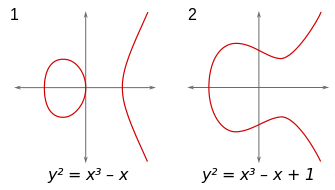
\includegraphics[width=200px]{ECC_1.png}
\end{figure}

Sulla sinistra una curva a due componenti, sulla destra una curva ad una componente.
Si hanno queste varianti in base alla cubica, si hanno infatti 3 radici che possono essere:
\begin{itemize}
    \item 3 reali $\implies$ curva a due componenti
    \item 1 reale e 2 complesse coniugate $\implies$ curva ad una componente
\end{itemize}

Si noti che sono sempre simmetriche rispetto all'asse delle $x$.
Se non imponessimo radici distinte avremmo curve con cuspidi o con nodi, in queste particolari curve la tangente non è detto che esista unica.

La simmetria viene dal termine $y^2$, infatti:
$$ P = (x,y) \in E(a,b) \implies y^2 = x^3 + ax + b $$
definiamo dunque:
$$ -P = (x,-y) \implies (-y)^2 = y^2 = x^3 + ax + b $$

NB: si pone 0 = -0

Dato $P=(x,y) \in E(a,b) $ si dice \emph{opposto} e si indica con $-P$ il punto $-P=(x,-y)$.

\subsection{Somma sulla curva ellittica}
Non ha nulla a che fare con la somma delle coordinate!
Si parte da una curva e studiamo l'intersezione con una retta: si possono avere al massimo 3 punti di intersezione.
Si risolve infatti il sistema:
\begin{equation}
    \begin{cases}
    y = mx + q \\
    y^2 = x^3 + ax + b
    \end{cases}
\end{equation}
si ottiene una cubica che ha al massimo 3 soluzioni.

Il sistema può essere risolto con:
\begin{itemize}
    \item 1 solo punto reale e due complessi coniugati
    \item 3 reali
\end{itemize}

Posso quindi prendere due punti sulla curva P e Q dato che ho due intersezioni esplicite ce ne sarà una terza per forza, chiamiamolo $R$. Il risultato di questa somma sarà $-R$ (per definizione).

\begin{figure}[H]
    \centering
    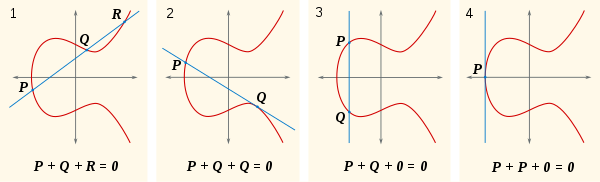
\includegraphics[width=325px]{ECC_2.png}
\end{figure}

Presi $P, Q, R \in E(a,b)$ se $P, Q, R$ sono disposti su una retta si pone:
$$ P + Q + R = 0 \implies P + Q = -R $$

Se $Q = P$ si considera la tangente alla curva nel punto $P$ (sempre definita per costruzione in quanto $4a^3+2tb^2 \neq 0$) e se ne vede l'intersezione con la curva.
Si noti che anche in questo caso se si fa passare una retta sull' estremo sinistro si ha una retta verticale e quindi la somma può dare il punto all'infinito.

\clearpage

\subsection{Proprietà della somma}
\subsubsection{Chiusura}
$$ \forall P, Q \in E(a,b): P+Q \in E(a,b) $$

\subsubsection{Elemento neutro}
$$ \forall P \in E(a,b): P + 0 = 0 + P = P $$

NB: Prendendo un punto $P$ e tracciando la retta all'infinito passante per $P$ l'altra intersezione è $-P$ quindi il risultato è $-(-P) = P$.

\subsubsection{Inverso (opposto)}
$$ \forall P \in E(a,b) \exists! Q \in E(a,b) : P + Q = 0 = Q + P$$
$$ Q = -P \implies P = (x,y), Q = (x, -y) $$

\subsubsection{Commutativa}
$$ \forall P, Q \in E(a,b) P + Q = Q + P $$

\subsubsection{Associativa}
$$ \forall P, Q, R \in E(a,b) (P + Q) + R = P + (Q + R) $$

\subsection{Formulazione algebrica}
Dati $P = (x_P, y_P)$, $Q = (x_Q, y_Q)$, $S = (x_S, y_S) = P+Q$ abbiamo:
\begin{itemize}
    \item $Q \neq \pm P$:
    \begin{equation}
        \begin{cases}
            x_S = \lambda^{2} - x_P - x_Q \\
            y_S = -y_P + \lambda(x_P - x_S) \\
            \lambda = \frac{y_Q - y_P}{x_Q - x_P}
        \end{cases}
    \end{equation}
    \item $P = Q$:
    \begin{equation}
        \begin{cases}
            x_S = \lambda^{2} - x_P - x_Q \\
            y_S = -y_P + \lambda(x_P - x_S) \\
            \lambda = \frac{3x_P^{2} + a}{2y_P}
        \end{cases}
    \end{equation}
    
    NB: se $y_P = 0$ $P+P=0$
    \item $Q = -P \implies P+Q = 0$
\end{itemize}

\subsection{Curve ellittiche su campi finiti}
\begin{minipage}{0.45\textwidth}
\centering
    Curve prime
    
    $K = Z_p$
    
    $p$ primo
    
    la caratteristica di $Z_p$ è $p$ quindi imponiamo $ p > 3 $
\end{minipage}
\hfill
\begin{minipage}{0.45\textwidth}
\centering
    Curve binarie
    
    $K = GF(2^m) , m \in \mathbb{N}$
    
    la caratteristica di K è uguale a 2 quindi non si può usare la forma normale di Weierstrass
\end{minipage}

\vspace{0.25cm}

Noi consideriamo solo le curve prime per le quali $4a^3 + 27b^2 \mod p \neq 0$ (CNS per gruppo Abeliano).

Ridefiniamo quindi la curva:
$$ E_p(a,b) = \{ (x,y) \in Z_p^2 \mid y^2 \mod p = x^3 + ax + b \mod p \} \cup \{0\} $$

Si noti che essendo in modulo si lavora sempre nel primo quadrante: $x, y \geq 0$.
La curva sarà ancora simmetrica ma non rispetto $y = 0$, bensì rispetto $y = \frac{p}{2}$ (parte intera inferiore).

Inoltre tutti i valori saranno in $[0, p-1]$ per il modulo.

Essendo simmetrica se $P=(x,y) \in E_p(a,b) \implies -P = (x, p-y) \in E_p(a, b)$.

NB: se $y^2 \equiv x^3 + ax + b$ allora $(p-y)^2 \equiv p^2 -2py + y^2 \equiv y^2$

Le formule della somma sono dunque le stesse ma si lavora in modulo (le divisioni diventano moltiplicazioni per l'inverso se non ci sono semplificazioni immediate, l'inverso c'è sempre perché lavoriamo modulo un numero primo).

\subsection{Ordine di una curva}
L'ordine di una curva è il numero di punti che la curva possiede.
Si hanno al massimo $p$ valori per $x$ quindi mi aspetto circa $2p + 1$ valori di $y$ soluzioni.
Ovviamente non tutti i valori nel campo hanno una radice quindi sono molti meno di $2p + 1$.
In genere in $Z_p$ i residui quadratici che definiscono un punto sulla curva sono $\frac{p-1}{2}$.

Il teorema di \emph{Hasse} ci dice che se $N$ è l'ordine della curva prima $E_p(a,b)$ allora:
$$ \mid N - (p+1) \mid \leq 2\sqrt{p}  $$

\subsection{Costruzione di una funzione one-way trap-door}
C'è una specie di parallelismo tra le operazioni in algebra modulare e le operazioni sulla curva ellittica:
\begin{itemize}
    \item la moltiplicazione diventa la somma tra due punti
    \item l'elevamento a potenza $k$ diventa la moltiplicazione di un punto per lo scalare $k$
\end{itemize}

Ci servono algoritmi di costo polinomiale quindi fare la somma $k$ volte non è praticabile (sarebbe esponenziale nella dimensione di $k$).
Possiamo quindi riusare l'algoritmo della esponenziazione veloce adattandolo: \emph{algoritmo dei raddoppi ripetuti}.

Eseguire $Q = kP$ si fa quindi in tempo polinomiale, trovare $k$ tale che $Q = kP$ invece è un problema difficile, si parla di \emph{logaritmo discreto sulle curve ellittiche}.

\subsection{Moltiplicazione scalare}
Calcolare $Q = kP$ è one-way, dati $k$ e $P$ è infatti facile calcolare $Q$ e si fa in O($\log k$):

Dato $Q = kP$, riscrivo $k$ in notazione binaria: 
$$ k = \sum_{i=0}^{t}k_i \cdot 2^i = (k_t,k_{t-1},\_,k_2,k_1,k_0) $$

Mi servono quindi $t+1 = \lfloor \log_2 k \rfloor + 1$ bit.
Si calcolano i vari $2P, 4P, \_, 2^tP$ in $t$ raddoppi ciascuno come raddoppio del punto precedente.
Si calcola $Q = \sum_{i : k_i = 1} (2^iP)$ in esattamente $t somme$.

O($t$) = O($\log_2 k)$ quindi lineare nella dimensione dell'input.

vediamo l'inverso della moltiplicazione scalare: dati $P$ e $Q$, sulla curva $E_p(a,b)$, trovare il più piccolo $k$ tale che: $Q = kP$. Non si conoscono algoritmi polinomiali ne sub-esponenziali per risolvere il problema.

\subsection{Protocollo DH su curve ellittiche}
Alice e Bob scelgono una curva ellittica prima (che soddisfi la condizione di gruppo Abeliano) ed un punto $B$ della curva che abbia ordine molto grande (l' ordine di un punto è il più piccolo $n$ tale che $nB=0$). $B$ sarebbe il generatore di DH.

NB: i punti e le curve sono già consigliate da NIST, non si devono quindi creare da zero.
Sono note e pubbliche.

L'algoritmo prosegue così:
\begin{itemize}
    \item Alice estrae $n_A < n$ casuale, calcola $P_A = n_AB$ e lo invia in chiaro a Bob
    \item Bob riceve $P_A$. Estrae $n_B < n$ casuale, calcola $P_B = n_BB$ e lo invia in chiaro ad Alice
    \item Alice riceve $P_B$ e calcola $S = n_AP_B = n_An_BB$
    \item Bob riceve $P_A$ e calcola $S = n_BP_A = n_Bn_AB$
\end{itemize}
ambo le parti hanno generato lo stesso $S$ e possono quindi generare la stessa chiave di sessione in vari modi (ad esempio $K = x_S \mod 256$).

Un crittoanalista non può fare nulla perché conosce $E_p(a,b), B, n, P_A, P_B$ ma non può trovare $n_A$ o $n_B$ se non risolvendo il problema del logaritmo discreto su curva ellittica.

NB: è sempre possibile un man-in-the-middle quindi la chiave va sempre estratta da un certificato!

NB: il sistema col logaritmo discreto su curva ellittica è facile sulla macchina quantistica.

\subsection{Scambio di messaggi cifrati}

\subsubsection{Algoritmo di Koblitz}
Innanzitutto bisogna preparare il messaggio affinché sia utilizzabile.
Si mappa quindi $m$ ad un punto della curva ellittica:
$$ m \xrightarrow{} P_m \in E_p(a,b) $$
si potrebbe pensare di usare $m$ come $x$ del punto ma potremmo incappare in una $y^2$ che non è un residuo quadratico, succede ben in $\frac{1}{2}$ delle volte.
Si usa quindi \emph{l'algoritmo di Koblitz} che prende un intero $n$ e restituisce un punto sulla curva.
E' un algoritmo randomizzato.

Si sceglie $h$ intero tale che $(m + 1) \cdot h < p$, eseguo quindi $i$ tentativi calcolando $x = m \cdot h + i$ con $0 \leq i < h$ e vedo se ottengo un punto valido:

\begin{verbatim}
    KOBLITZ(m, h, E):
        for(i=0; i < h; i++):
            x = m*h + i
            z = (x^3 + E.a*x + E.b) mod E.p
            if z è un residuo quadratico:
                y = sqrt(z)
                return (x,y)
        return "failure"
\end{verbatim}

La probabilità di fallimento è $\approx \frac{1}{2}^h$, quindi la probabilità di successo è circa $\approx 1 - \frac{1}{2}^h$.

Se ci è andata male si modifica il messaggio e si riprova.

In fase di decriptazione si ritrovano $(x,y)$ ma $x$ non è il messaggio vero, si deve infatti calcolare:
$$ m = \lfloor \frac{x}{h} \rfloor = \lfloor \frac{mh+i}{h} \rfloor = \lfloor m + \frac{i}{h} \rfloor = m $$

\subsubsection{Cifratura e decifratura}
Presi una curva $E_p(a,b)$ ed un suo punto $B$ con ordine elevato $n$, preso inoltre $h$ da usare per Koblitz ogni utente deve generare la sua coppia chiave pubblica-chiave privata.

\begin{itemize}
    \item Bob U estrae $n_{BOB} < n$, chiave privata
    \item calcola $P_{BOB} = n_{BOB} \cdot B$, chiave pubblica
\end{itemize}

Ora Alice vuole inviare un messaggio cifrato a Bob:
\begin{itemize}
    \item prende il messaggio $m$ e lo mappa ad un punto della curva $P_m \in E_p(a,b)$
    \item sceglie un intero a caso $r$, calcola $V = r \cdot B$. $V$ è un punto che \emph{protegge} $r$
    \item calcola $W = P_m + r \cdot P_{BOB}$
    \item invia la coppia $<V,W>$
\end{itemize}

Bob deve quindi decifrare il messaggio:
\begin{itemize}
    \item riceve la coppia $<V,W>$
    \item calcola:
        $$ W -n_{BOB} \cdot V = P_m + r \cdot P_{BOB} - n_{BOB} \cdot r \cdot B = $$
        $$ = P_m + \cancel{r \cdot n_{BOB} \cdot B} - \cancel{r \cdot n_{BOB} \cdot B} = P_m$$
    \item ottiene il messaggio calcolando:
        $$ m = \lfloor \frac{x}{h} \rfloor $$
\end{itemize}

La sicurezza è legata al logaritmo discreto in quanto Eve può:
\begin{itemize}
    \item partendo da $V$ trovare $r$ e decifrare con:
    $$W - r\cdot P_{BOB} = P_m + \cancel{r \cdot P_{BOB}} - \cancel{r \cdot P_{BOB}} = P_m$$
    ma per trovare $r$ bisogna risolvere $V = r \cdot B$
    
    \item partendo da $P_{BOB}$ può trovare $n_{BOB}$ e decifrare esattamente come fa Bob, ma anche qui c'è da risolvere $P_{BOB} = n_{BOB} \cdot B$
\end{itemize}

Si noti che inoltre $r$ è one-time quindi se si dovessere passare a brutare converrebbe comunque andare a ricavare la chiave privata.

\subsection{Sicurezza}
Per attaccare RSA, DH, El Gamal (su algebra modulare) si hanno algoritmi di costo O($2^{\sqrt{b \log b}}$) con $b$ numero di bit del modulo.

Questi attacchi sono basati sull' \emph{index calculus} in quanto si ha una struttura di campo.
Per attaccare protocolli su curve ellittiche invece si ha un costo O($2^{\frac{b}{2}}$) con $b$ bit dell'ordine di $B$, non essendo un campo ma un gruppo Abeliano si pensa che le tecnice usate per l'algebra modulare non verranno mai trasposte anche qui.
\section{Identificazione, autenticazione e firma digitale}

L' \emph{identificazione} prevede che un sistema isolato o in rete debba essere in grado di accertare l'identità di un utente che richiede di accedere ai suoi servizi.

L' \emph{autenticazione} prevede che il destinatario di un messaggio possa essere in grado di accertare:
\begin{itemize}
    \item l'identità del mittente
    \item l'integrità del crittogramma ricevuto (che non sia stato modificato, che non sia stato sostituito)
\end{itemize}

NB: identificazione $\subset$ autenticazione

La \emph{firma digitale} ci permette invece:
\begin{itemize}
    \item il mittente non può negare di aver inviato il messaggio $m$: \emph{non ripudiabilità}
    \item il destinatario deve essere in grado di autenticate il messaggio: \emph{autenticazione}
    \item il destinatario non deve poter sostenere che $m' \neq m$ è il messaggio inviato dal mittente
\end{itemize}
In fine tutto questo deve essere verificabile da terzi!

Non sono modalità indipendenti, ciascuna estende le precedenti!
Sono funzionalità utilizzate per contrastare gli attacchi attivi.

Ci sono realizzazioni sia su cifrari simmetrici che asimmetrici, noi vedremo queste ultime versioni.

\subsection{Funzioni hash}
Una funzione hash: $f: X \xrightarrow{} Y$ è una funzione tale che:
$$ n = \mid X \mid >> m = \mid Y \mid $$

Essendo non iniettiva: $ \exists X_1, X_2, \_, X_m \subseteq X$ disgiunti tali che: 
$$ X = X_1 \cup X_2 \cup \_ \cup \_ X_m $$
$$ \forall i, x : x \in X_i : f(x) = y $$
ogni insieme $X_i$ è l'insieme di collisioni e si vuole che le dimensioni dei vari $X_i$ sia più omogenea possibile.
Quindi due elementi estratti a caso da $X$ hanno probabilità circa $\frac{1}{m}$ di avere la stessa immagine $y$.

Inoltre si vuole che immagini \emph{simili} tra loro appartengano a sottoinsiemi diversi.
Bisogna gestire le collisioni.
Queste sono le richieste per una buona funzione di hash

\subsection{Funzioni hash one-way}
Per le applicazioni crittografiche si devono avere le seguenti proprietà:
\begin{itemize}
    \item $\forall x \in X$ è computazionalmente facile calcolare $y = f(x)$
    \item one-way: per la maggior parte degli $y \in Y$ è computazionalmente difficile determinare $x \in X$ tale che: $f(x) = y$
    \item \emph{claw-free}: è computazionalmente difficile determinare $<x_1, x_2>$ in $X$ tale che: $f(x_1)=f(x_2)$ 
\end{itemize}

\subsubsection{MD5 (Message Digest v5)}
Si tratta di una famiglia di algoritmi.
Sono stati pubblicati MD2, MD4, MD5.
Nei primi due furono trovate falle e Rivest propose MD5 nel 1992.

Riceve in input un sequenza $S$ di 512 bit e produce un'immagine di 128 bit.
Si \emph{digerisce} la sequenza riducendone la lunghezza ad $\frac{1}{4}$.

Non resiste alle collisioni e nel 2004 è uscito di scena con debolezze varie.

Si considera severamente compromesso (anche dallo stesso Rivest).

Si usa ancora in altri contesti non crittografici.

\subsubsection{RIPEMD-160}
E' la versione matura dell'MD*. Nata nel 1995 produce immagini di 160 bit e non presenta i difetti di MD5.

\subsubsection{SHA (Secure Hash Algorithm)}
Progettata dal NIST ed NSA nel 1993.
Opera su sequenze lunghe fino a $2^{64}$ bit e produce immagini di 160 bit.
E' crittograficamente sicura.
La prima versione: SHA-0 conteneva debolezze e fu quindi rivista portando allo SHA-1.

Sono poi stati creati SHA-2: altri 4 algoritmi caratterizzati da digest più lunghi.

Nel 2007 a causa dei problemi di MD5 e SHA-0 il NIST ha richiesto nuovi standard e nel 2012 è stato selezionato un algoritmo che è diventano SHA-3, pubblicato ufficialmente nel 2015.

\subsubsection{SHA-1}
Opera su sequenze fino a $2^{64}-1$ bit e produce immagini di 160 bit.
E' largamente usata nei protocolli crittografici anche se non è più certificata come standard.

Opera su blocchi di 160 bit contenuti in un buffer di 5 registri da 32 bit ciascuno in cui sono caricati inizialmente dei valori pubblici.
Il messaggio $m$ viene poi concatenato con una sequenza di padding che ne rende la lunghezza multipla di 512 bit.

Il contenuto dei registri varia nel corso dei cicli successivi in cui questi valori si combinano tra loro e con blocchi di 21 bit provenientei da $m$.
Alla fine i registri contengono SHA-1($m$).

\subsection{Identificazione su canali sicuri}
Supponiamo di avere un utente che vuole accedere alle risorse su un calcolatore.
Per identificarsi usa username e password.
Supponiamo che viaggiare su un canale sicuro, le uniche fonti di attacco sono quindi sul calcolatore remoto.
Per evitare problemi sul server remoto non si memorizzano le password in chiaro ma un loro hash.
In particolare sui sistemi UNIX quando un utente $U$ fornisce per la prima volta una password $P$ il sistema associa ad $U$ due sequenze binarie:
\begin{itemize}
    \item $S$: seme prodotto da un generatore pseudocasuale
    \item $Q = h(PS)$: hash della concatenazione di $P$ ed $S$
\end{itemize}

Ad ogni successiva connessione il sistema prende la password, la concatena ad $S$, ne esegue l'hash e controlla che sia uguale all'hash memorizzato.

In questa maniera un accesso al file delle password non rivela informazioni importanti.

\subsection{Protezione del canale}
Se il canale è insicuro la password può essere intercettata durante la sua trasmissione in chiaro.
Vediamo quindi un sistema di \emph{identificazione} basato su chiave pubblica e privata.

Per esempio siano $<e,n>$, $<d,n>$ le chiavi pubblica e privata di un utente $U$ che richiede l'accesso ai servizi offerti dal sistema $S$.
\begin{itemize}
    \item $S$ genera un numero casuale $r < n$ e lo invia in chiaro a $U$
    \item $U$ calcola:
    $$ f = r^d \mod n $$
    \emph{firma di $U$ su $r$}
    \item $S$ verifica la correttezza del valore ricevuto calcolando:
    $$ f^e \mod n $$
    e verificando l'uguaglianza. Se avviene l'identificazione ha successo
\end{itemize}

Se $S$ non è trusted potrebbe inviare un $r$ particolare, anziché randomico, per cercare di carpire informazioni sulla chiave privata!

Si tratta di invertire le operazioni di crittazione e decifrazione rispetto all' RSA, ciò è possibile poiché è commutativo:
$$ (x^e \mod n)^d \mod n = (x^d \mod n)^e \mod n = x $$

Inoltre $f$ può essere generata solo da $U$ che possiede $<d, n>$.

Per eseguire l'autenticazione invece si usa il MAC: \emph{message authentication code}.
\begin{itemize}
    \item mittente e destinatario concordano una chiave segreta $k$
    \item il mittente allega al messaggio un MAC:
    $$ A(m,k) $$
    allo scopo di garantire la provenienza e l'integrità del messaggio.
    Spedisce quindi $<m, A(m,k)>$ in chiaro oppure spedisce $<C(m,k'),A(m,k)>$ frutto di una cifratura
    \item il destinatario entra in possesso di $m$, essendo a conoscenza di $A$ e $k$ ricalcola $A(m,k)$ e ne confronta il valore con quello inviato dal mittente. Se i MAC corrispondono allora ha successo
\end{itemize}

\subsection{MAC}
Deve essere una immagine breve del messaggio che si può ottenere solo se si è a conoscenza del valore comune $k$.
Ci sono varie implementazioni basate su cifrari asimmetrici, simmetrici e funzioni hash one-way.
In particolare la versione one-way prevede:
$$ A(m,k) = h(mk) $$
con $h$ una funzione hash one-way.

E' sicuro in quanto $k$ viaggia nel MAC ed anche se venisse scoperto non è invertibile in maniera semplice.
Non può nemmeno sostituire tutto in quanto dovrebbe corredare il messaggio di un nuovo MAC che però non può calcolare essendo all' oscuro del valore di $k$.

NB: se si usa un cifrario a blocchi in modalità CBC si può usare l'ultimo blocco come MAC in quanto è funzione dell'intero messaggio.

\subsection{Firma manuale}
\begin{itemize}
    \item E' autentica e non falsabile: prova che chi la ha prodotta è chi ha sottoscritto il documento
    \item Non è riutilizzabile: è legata al documento su cui è stata apposta
    \item il documento non è alterabile: chi ha prodotto la firma è sicuro che questa si riferirà solo al documento sottoscritto nella sua forma originale
    \item non può essere ripudiata da chi l'ha apposta costituendo prova legale di un accordo o dichiarazione
\end{itemize}

\subsection{Firma digitale}
Non può banalmente essere la digitalizzazione di un documento originale firmato manualmente (si potrebbe banalmente tagliare ed incollare su un altro documento).
Deve quindi avere una forma che dipenda dal documento per essere inscindibile.
Ci sono protocolli che si basano sia su cifrari simmetrici che asimmetrici

\subsection{Protocollo 1: messaggio in chiaro e firmato (DH)}
L'utente $U$ dispone di una $K_{upriv}$ e $K_{upub}$. $C$ e $D$ sono funzioni di cifratura e decifratura di un cifrario asimmetrico.
La firma funziona:
\begin{itemize}
    \item $U$ genera la firma 
    $$f = D(m, k_{upriv})$$
    \item spedisce all'utente $<U,m,f>$
    \item l'utente riceve $<U,m,f>$ e calcola 
    $$C(f, K_{upub}) = m$$
    e verifica che il risultato sia proprio $m$
\end{itemize}

L'indicazione del mittente $U$ consente a $V$ di selezionare la $K_{upub}$ da utilizzare.
Per far funzionare questo meccanismo è importante che $C$ e $D$ siano commutative.

Questo protocollo soddisfa i requisiti della firma digitale:
\begin{itemize}
    \item è autentica e non falsabile in quanto $K_{upriv}$  è nota solo al mittente, per falsificare la firma bisogna conoscere $K_{upriv}$ ma è difficile
    \item il documento non può essere alterato in quanto $m$ e $f$ sarebbero inconsistenti
    \item $U$ non può ripudiare la firma perché può averla prodotta solo lui
    \item la firma non è riutilizzabile in quanto $f$ è immagine di $m$
\end{itemize}

La verifica la possono fare tutti, tuttavia non ha nessuna cifratura del messaggio in quanto pur cifrando il messaggio posso ricavarlo dalla firma.

\subsection{Protocollo 2: messaggio cifrato e firmato}
\begin{itemize}
    \item $U$ genera la firma:
    $$ f = D(m, K_{upriv}) $$
    per $m$
    \item si calcola il crittogramma firmato:
    $$ c = C(f, K_{vpub}) $$
    con la chiave del destinatario
    \item invio $<U, c>$
    \item $V$ riceve la coppia $U, c$ e la decifra:
    $$ D(c, K_{vpriv}) = f $$
    \item verificando la firma si ottiene anche il messaggio:
    $$ C(f, K_{upub}) = C(D(m, K_{upriv}), K_{upub}) = m $$
\end{itemize}

Ci servono quindi:
$$ <d_u, n_u>, <e_u, n_u> \textbf{ chiavi di U} $$
$$ <d_v, n_v>, <e_v, n_v> \textbf{ chiavi di V} $$

L'utente U:
\begin{itemize}
    \item firma il messaggio: $f = m^{d_u} \mod n_u$
    \item cifra il messaggio: $c = f^{e_v} \mod n_v$
    \item spedisce la coppia: $<U, c>$
\end{itemize}

L'utente V:
\begin{itemize}
    \item riceve e decifra: $f = c^{d_v} \mod n_v$
    \item decifra $f$ con $k_{upub}$: $f^{e_u} \mod n_u = m$
\end{itemize}

Se $m$ è significativo concludo che è autentico.

Per la correttezza del procedimento è necessario che $n_u \leq n_v$ affinché sia vero che $f < n_v$ e quindi $f$ possa essere cifrato correttamente.
In questo modo tuttavia $V$ non può rispondere in quanto dovrebbero avere $n_u = n_v$ ma è poco sicuro e probabile.

Possiamo ovviare quindi dando ad ogni utente due chiavi distinte: una per la firma $< H$ ed una per la cifratura $> H$ con $H$ pubblico e molto grande.

NB: si può attaccare se ci si procura la firma di un utente su un messaggio apparentemente privo di senso

\subsubsection{Attacco 1}
Supponiamo che un utente $U$ invii una risposta automatica (ack) al mittente ogni volta che riceve un messaggio $m$, e che questo messaggio sia il crittogramma della firma di $U$ su $m$.
Un crittoanalista attivo $X$ può decifrare i messaggi inviati a U:
\begin{itemize}
    \item $X$ intercetta $c$ firmato e crittografato inviato da $V$ a $U$, lo rimuove dal canale e lo rispedisce a $U$ con identificativo $X$. (cancella $<V,c>$ ed invia $<X,c>$)
    \item $U$ spedisce un ack ad $X$ in risposta
    \item $X$ usa l' ack per risalire al messaggio $m$ applicando le funzioni del cifrario con le chiavi pubbliche di $V$ e di $U$.
\end{itemize}

In particolare succede:
\begin{itemize}
    \item $V$ invia $c$ a $U$:
        \begin{equation}
            \begin{cases}
                c = C(f, K_{upub}) \\
                f = D(m, K_{vpriv})
            \end{cases}
            \implies <V,c>
        \end{equation}
    \item $X$ intercetta $c$, lo rimuove e rispedisce $<X,c>$
    \item $U$ decifra $c$:
    $$ f = D(c, K_{upriv}) $$
    e verifica la firma con la chiave pubblica di X ottenendo:
    $$ m' = C(f, K_{xpub}) $$
    \item $m' \neq m$ è privo di senso ma manda automaticamente l'ack $c'$ ad $X$:
    $$ f' = D(m', K_{upriv}) $$
    $$ c' = C(f', K_{xpub}) $$
    \item $X$ usa $c'$ per risalire ad $m$: decifra $c': D(c', K_{xpriv}) = f'$ e verifica $f': C(f', K_{upub}) = m'$. Da $m'$ ricava $f: D(m', K_{xpriv})=f$, verifica $f: C(f, K_{vpub}) = m$
\end{itemize}

Per evitare l'attacco si deve evitare l'ack automatico inviandolo solo se il messaggio ha senso.

\subsection{Protocollo resistente agli attacchi}
Si evita di firmare il messaggio!
Si crea un hash del messaggio (SHA) con una funzione hash one-way e vi si appone la firma sopra.
La firma non è quindi più soggetta a giochi algebrici.
\begin{itemize}
    \item il mittente $U$ calcola $h(m)$ e genera:
    $$ f = D(h(m), K_{upriv})$$
    \item calcola separatamente:
    $$ c = C(m, K_{vpub}) $$
    \item spedisce a $V$ la tripla: $<U, c, f>$
\end{itemize}

La decifrazione e verifica invece:
\begin{itemize}
    \item $V$ riceve e verifica $<U, c, f>$
    \item decifra il crittogramma $c: m = D(c, K_{upriv})$
    \item calcola $h(m)$ e $C(f, K_{upub})$ e ne controlla l'uguaglianza, se sono uguali il messaggio è autentico
\end{itemize}
La firma si calcola più velocemente.

\subsection{Attacchi man-in-the-middle}
Le chiavi di cifratura sono pubbliche e non richiedono un incontro diretto per il loro scambio.
Un crittoanalista attivo può quindi intromettersi nella fase iniziale comportandosi come $V$ agli occhi di $U$ e come $U$ agli occhi di $V$.
\begin{itemize}
    \item $U$ richiede a $V$ la sua chiave pubblica
    \item $X$ intercetta la risposta contenente $K_{vpub}$ e la sostituisce con la sua chiave pubblica $K_{xpub}$
    \item $X$ si pone in ascolto in attesa dei crittogrammi spediti da $U$ a $V$ cifrati mediante $K_{xpub}$
    \item $X$ rimuove dal canale ciascuno dei crittogrammi, li decripta e li cifra con $K_{vpub}$ trafugata all'inizio, rispedendola a $V$
    \item $U$ e $V$ non si accorgono di nulla se il tutto è fatto velocemente
\end{itemize}

\subsection{Certification of Authority - CA}
Sono infrastrutture/enti che garantiscono la validità delle chiavi pubbliche e ne regolano l'uso gestendo la distribuzione delle chiavi a chi vuole comunicare.
La CA autentica l'associazione $<$utente, chiave pubblica$>$ emettendo un certificato digitale.
Il certificato consiste della chiave pubblica e di una lista di informazioni relative al suo proprietario opportunamente firmate dalla CA.

Mantiene quindi un archivio accessibile a tutti ma protetto da scritture non autorizzate.
La chiave della CA è nota agli utenti che la mantengono protetta e la utilizzano per verificare la firma della stessa CA.

\subsection{Certificato digitale}
Si compone principalmente di:
\begin{itemize}
    \item indicazione del formato (numero di versione)
    \item nome della CA che lo ha rilasciato
    \item numero seriale che lo individua univocamente nella CA emittente
    \item specifica dell'algoritmo usato dalla CA per creare la firma digitale
    \item periodo di validità
    \item nome ed altre informazioni dell'utente a cui si riferisce il certificato
    \item nome dell'algoritmo, parametri e chiave pubblica usati dall'utente per cifratura e firma
    \item firma della CA su tutto quanto
\end{itemize}

Se $U$ vuole comunicare con $V$ può richiedere $K_{vpub}$ alla CA oppure direttamente a $V$ e poi lo convalida tramite la CA.

Dato che $U$ conosce $K_{CA-pub}$ può controllarne l'autenticità e la validità.
Se tutto va a buon fine la comunicazione parte.

Ci si può mettere nel mezzo solo falsificando la certificazione ma si assume che la CA sia fidata.

Esistono varie CA organizzate ad albero, la verifica quindi è più complicata in quanto si cerca il primo antenato comune tra le CA di $U$ e di $V$. Ogni utente poi mantiene in cache una copia dei certificati richiesti ed una copia di $K_{CA-pub}$ per non doverla richiedere.

\subsection{Protocollo 4: messaggio cifrato, firmato in hash e certificato}
Il mittente $U$:
\begin{itemize}
    \item si procura $cert$ di V

    \item calcola $h(m)$ e firma:
    $$ f = D(h(m),K_{upriv}) $$

    \item calcola $c$:
    $$ c = C(m, K_{vpub}) $$

    \item spedisce $<cert_U$, c, f$>$ ($cert_U$ contiene $K_{upub}$)
\end{itemize}

Il destinatario $V$:
\begin{itemize}
    \item riceve $<cert_U$, c, f$>$ e verifica l'autenticità di $cert_U$ (e di $K_{upub}$) tramite la CA.

    \item decifra il crittogramma:
    $$ m=D(c, K_{vpriv}) $$

    \item verifica l'autenticità della firma:
    $$ c(f, K_{upub}) = h(m) $$
\end{itemize}

La catena ha un punto debole: i certificati non più validi; è quindi cruciale controllare periodicamente con la CA i certificati scaduti.
\section{Zero Knowledge}

\subsection{Idea Generale}
Un protoccolo \emph{zero knowledge} è un protocollo che permette ad un \emph{Prover} di dimostrare di avere una certa conoscenza ad un \emph{Verifier} senza inviare alcuna informazione se non l'evidenza di avere questa conoscenza.

Facciamo un esempio concreto: supponiamo che Peggy dica di poter sapere di quanti granelli di sabbia si compone una spiaggia semplicemente osservandola e che Victor voglia controllare la veridicità di questa affermazione senza arrivare alla totale certezza ma avvicinandosi tramite una probabilità prossima ad 1. Supponiamo inoltre che Peggy risponda:

\begin{itemize}
    \item 1 se il numero è dispari
    \item 0 se il numero è pari
\end{itemize}

Immaginiamo il seguente algoritmo:

\begin{verbatim}
    for i = 1 to k{
        P si volta
        V sceglie e in {0, 1} casualmente
        if (e == 0)
            V rimuove un granello di sabbia
        V chiede a P il nuovo b[i]
        if ((e == 0 && b[i] != b[i-1]) || 
            (e == 1 && b[i] == b[i-1]))
            vado alla prossima iterazione
        else
            P è un impostore -> STOP
    }
\end{verbatim}

la probabilità, al passo k, che Peggy sia un impostore è pari a:
$$
    \frac{1}{2^k}
$$
altresì la probabilità che Peggy dica il vero è:
$$
    1 - \frac{1}{2^k}
$$

Se il Prover è onesto non ha problemi a rispondere a tutte le iterazioni in maniera corretta, se non lo è può solo provare ad indovinare, quindi la probabilità di vincere imbrogliando è pari a quella di indovinare una sequenza di k bit casuali. 


\subsection{Proprietà generali}
\subsubsection{Completezza}
Se ciò che dice P è vero ed il verificatore è onesto il verificatore deve sempre accettare la dimostrazione.
\subsubsection{Correttezza}
Se il prover dice il falso, il verificatore può essere ingannato con probabilità $\leq \frac{1}{2^k}$ con $k$ scelto da V.
\subsubsection{Conoscenza-zero}
Se l'affermazione di P è vera V (anche se disonesto) non può acquisire alcuna informazione se non il fatto che P ha la conoscenza che dice di avere.

\subsection{Protocollo di Fiat-Shamir}
E' un protocollo di autenticazione nel quale P dimostra a V la sua identità senza svelare altre informazioni. Si basa sulla difficoltà di calcolo di $\sqrt{x} \mod n$ con $n$ composto. 

\subsubsection{Generazione delle chiavi}
\begin{itemize}
    \item P genera $p$ e $q$ numeri primi (grandi)
    \item calcola $n = p \cdot q$
    \item sceglie $s$ numero casuale tc $s < n$
    \item calcola $t = s^2 \mod n$
\end{itemize}
La coppia $<t,n>$ costituisce la chiave pubblica da distribuire mentre la terna $<p, q, s>$ costituisce la chiave privata.

\subsubsection{Autenticazione}
L'algoritmo di autenticazione prevede $k$ iterazioni con $k$ scelto da V:
\begin{itemize}
    \item V chiede a P di iniziare una iterazione
    \item P genera un intero $r < n$, calcola $u = r^2 \mod n$ e comunica $u$ a V
    \item V sceglie casualmente $e \in \{1, 0\}$ e lo comunica a P
    \item P calcola $z = r \cdot s^e \mod n$ e lo comunica a V
    \begin{itemize}
        \item $e = 0 \implies z = r$
        \item $e = 1 \implies z = r \cdot s \mod n$
    \end{itemize}
    \item V calcola $x = z^2 \mod n$ e controlla se $x == (u \cdot t^e \mod n)$
    \begin{itemize}
        \item se sono uguali si passa alla prossima iterazione
        \item se sono diversi P è un impostore
    \end{itemize}
\end{itemize}

Si noti che se tutto è corretto:
$$
    x = z^2 = (r \cdot s^e)^2 = r^2 \cdot s^{2 \cdot e} = u \cdot t^{e} \mod n
$$

\subsubsection{Completezza}
La completezza si ottiene, si noti infatti che:
$$ e = 0 \implies x = u \mod n $$
$$ e = 1 \implies x = u \cdot t \mod n $$
quindi se P è onesto passa tutte le prove e V accetta la dimostrazione

\subsubsection{Correttezza}
La correttezza si ottiene: supponiamo che P preveda correttamente il prossimo valore di $e$ scelto dal verificatore:
\begin{itemize}
    \item se prevede $e = 1$: sceglie $r$ casualmente ma invia $u = \frac{r^2}{t} \mod n$, successivamente manderà $z = r \mod n$. V andrà quindi a verificare: $x = z^2 = r^2$, $u \cdot t = \frac{r^2}{t} \cdot t = r^2 \implies x = u \cdot t \mod n$
    \item se prevede $e = 0$: esegue l'algoritmo corretto infatti $x = z^2 = r^2$, $u \cdot t^e = u = r^2 \implies x = u \mod n$
\end{itemize}
questo però è subordinato al poter prevedere il corretto valore di $e$ che per $k$ scelto equivale a $\frac{1}{k^2}$.

\subsubsection{Zero Knowledge}
Sì ma la dimostrazione non la vediamo

\subsection{Perché?}
Questo protocollo di autenticazione è un protoccollo sicuro da entrambi i lati, sia per chi si deve far riconoscere che per chi autentica le richieste. Pensiamo ad una generica autenticazione tramite crittografia asimmetrica:
\begin{itemize}
    \item il client si vuole autenticare presso un server
    \item il server dispone della chiave pubblica del client, chiede quindi al client di firmare un messagio $r$ casuale
    \item il client riceve $r$, lo firma e lo restituisce al server
    \item il server verifica la firma e se è corretta l'autenticazione è avvenuta
\end{itemize}
In questo scenario ci si deve fidare del server in quanto si prende un messaggio arbitrario e lo si firma con la propria chiave privata, questo tuttavia potrebbe essere problematico in quanto possono esistere degli input malevoli che permettono di ottenere informazioni circa la chiave privata del client. Un protocollo a zero knowledge invece pone entrambi i lati della comunicazione sullo stesso piano di diffidenza.

\clearpage
\section{Protocollo SSL}
SSL (Secure Socket Layer) è alla base dei protocolli più diffusi nelle comunicazioni sicure.
Garantisce \emph{confidenzialità} e \emph{affidabilità} delle comunicazioni su internet proteggendole da intrusioni, modifiche e falsificazioni.
Sviluppato inizialmente da Netscape per mettere in sicurezza HTTP è progettato in modo da permettere la comunicazione tra computer che non conoscono le reciproche funzionalità.
Oggi è sostituito dal TLS (Transport Layer Security) che è una variante con qualche modifica.

Garantisce la confidenzialità tramite l'uso di un sistema ibrido: cifrario asimmetrico per lo scambio delle chiavi ed uno simmetrico per la cifratura delle comunicazioni.

Garantisce l'autenticazione dei messaggi accertando l'identità dei due partner attraverso sia un cifrario asimmetrico che tramite certificati digitali con un MAC.

Si trova tra il TCP (trasporto) e HTTP (applicazione) ma è totalmente indipendente dal protocollo applicativo sovrastante (HTTPS = HTTP su SSL).

SSL è organizzato in:
\begin{itemize}
    \item \emph{SSL record}: è il livello più basso, connesso direttamente al protocollo di trasporto ed ha l'obiettivo di incapsulare i dati spediti dai livelli superiori assicurando confidenzialità ed integrità.
    \item \emph{SSL handshake}: instaura e mantiene i parametri poi usati da SSL record. Permette quindi di autenticarsi, negoziare gli algoritmi di cifratura e firma, stabilire le chiavi dei singoli algoritmi crittografici e per il MAC.
\end{itemize}

C'è uno scambio di messaggi preliminare per la creazione del canale sicuro, nel frattempo client e server si identificano a vicenda e cooperano per costruire le chiavi simmetriche. Vediamo singolarmente le fasi.

\subsection{Fasi di SSL}

\subsubsection{client hello}
$U$ manda ad $S$ un messaggio con il quale si richiede la connessione SSL, si specificano i cifrari e meccanismi che $U$ supporta e le prestazioni di sicurezza richieste.
Si aggiungono in fine dei byte casuali. Tutto questo è mandato in chiaro!

Es: SSL\_RSA\_WITH\_AES\_CBC\_SHA1:
\begin{itemize}
    \item RSA: per lo scambio delle chiavi di sessione
    \item AES: come cifratura simmetrica
    \item CBC: come composizione dei blocchi
    \item SHA1: come funzione hash per il MAC
\end{itemize}
Questo è un esempio di \emph{cipher suite}

\subsubsection{server hello}
Riceve il messaggio dell'utente, seleziona una cipher suite che anche lui supporta ed invia al client un messaggio che specifica la sua scelta. Appende dei byte casuali alla risposta. Anche questo è mandato in chiaro!

NB: Se $U$ non riceve il server hello interrompe la comunicazione

\subsubsection{Autenticazione}
$S$ si autentica con $U$ inviandogli il proprio certificato digitale (e gli eventuali altri certificati fino al primo nodo comune nella catena delle CA).

NB: se i servizi offerti da $S$ devono essere protetti negli accessi anche $S$ può richiedere a $U$ di autenticarsi inviando il suo certificato digitale. Avviene raramente in quanto la maggior parte degli utenti non ha un proprio certificato e in genere ci si accerta dell'identità di un utente in un secondo modo (autenticazione sul sito web ad esempio).

\subsubsection{server hello done}
Messaggio con il quale il server sancisce la fine degli accordi sulla cipher suite ed i parametri crittografici associati.

\subsubsection{Controllo da parte del client}
$U$ accerta l'autenticità del certificato ricevuto da $S$ tramite la data, tramite la CA che lo ha firmato, ecc. Estrae la chiave pubblica dal certificato. Costruisce il \emph{pre-master secret} costituito da una nuova sequenza casuale di byte. Lo cifra con la chiave pubblica estratta dal certificato. Spedisce il crittogramma ad $S$.

\subsubsection{Costruzione del master secret}
Sempre il client costruisce il \emph{master secret} partendo dal pre-master secret, altre stringhe note ed i byte casuali di client hello e server hello.
Applica a tutte queste sequenze delle funzioni hash one-way secondo una combinazione opportuna.
Questa sarà il master secret.

\subsubsection{Ricostruzione del master secret}
Anche il sistema si calcola localmente il master secret dopo aver ottenuto il pre-master secret decriptandolo con la sua chiave privata.
Ora entrambi gli utenti hanno il master secret!

\subsubsection{Autenticazione dell'utente}
Se all'utente $U$ è richiesto un certificato ed egli non lo possiede il sistema interrompe l'esecuzione del protocollo.
Altrimenti $U$ invia il proprio certificato allegando master secret e la SSL-history (tutti i messaggi scambiati fino a quel momento) firmate con la sua chiave privata.
$S$ controlla certificato ed history.

\subsubsection{finished}
E' il primo messaggio protetto da master secret e cipher suite accordati. Il messaggio è costruito da $U$ ed inviato ad $S$ e poi costruito da $S$ ed inviato a $U$. Il messaggio ha la stessa strutura ma cambiano i dati (la history).
La costruzione avviene:
\begin{itemize}
    \item master secret, messaggi di handshake, identità del mittente ($U$ o $S$)
    \item si hasha la stringa ottenuta sia con SHA-1 che con MD5, le due stringhe ottenute sono il messaggio \emph{finished}.
\end{itemize}
Il messaggio è diverso in quanto $S$ aggiunge anche la finished ricevuta da $U$ in quanto ora fa parte della history.
Non sono ovviamente invertibili perché costruiti tramite hash.

Il master secret viene usato per creare le chiavi:
\begin{itemize}
    \item chiave segreta per il cifrario simmetrico
    \item chiave per l'autenticazione del messaggio (MAC)
    \item initialization vector per il CBC
\end{itemize}

Le terne di chiavi di $U$ ed $S$ sono diverse tra loro ma note ad entrambi, ciascuno usa la propria, quindi aumenta la sicurezza.

Successivamente i parametri vengono passati al SSL Record che si occupa del vero e proprio dialogo dei dati suddividendo i dati in blocchi, aggiungendo un MAC ad ogni blocco, cifrato con il protocollo simmetrico scelto e trasmesso al protocollo di trasporto sottostante.

Il destinatario esegue il contrario.

\subsection{Sicurezza di SSL}
Nei passi di hello i due partner creano e si inviano sequenze casuali per costruire la master secret, questo risulta in chiavi diverse ogni volta.
Un crittoanalista non può riutilizzare i messaggi catturati sul canale per sostituirli a S successivamente.

L'SSL record successivamente numera ogni blocco in maniera incrementale e lo autentica tramite MAC.
Un blocco non può essere modificato in quanto il MAC è hash di:
\begin{itemize}
    \item contenuto
    \item numero sequenziale del blocco
    \item chiave del MAC
    \item altre stringhe note e fissate a priori
\end{itemize}

MAC e messaggio sono cifrati quindi prima di poterli alterare va forzato il cifrario.

Non si possono eseguire man-in-the-middle in quanto si usano i certificati.

Il pre-master secret è inviato cifrato con chiave pubblica quindi è sicuro.

Quindi solo $S$, proprietario della chiave privata associata al certificato può recuperare la pre-master key e quindi entrare in comunicazione con $U$.

Anche $U$ può essere autenticato se necessario.
Se è richiesto ma non avviene la comunicazione salta.
L'opzionalità di questa autenticazione ha reso usato questo protocollo in quanto può essere autenticato in altri modi, magari lato applicazione.

Le sequenze sono generate a partire da byte casuali quindi una sua predicibilità metterebbe a rischio tutto.

Il messaggio finished contiene tutta la history e quidi permette un ulteriore controllo finale.

E' sicuro almeno quanto il cifrario più debole della cipher suite, ma non ci sono cifrari deboli lasciati dentro.


\section{Quantum Distribution Key (QDK)}
E' un modo alternativo al DH per lo scambio di chiavi.
Permette di scambiare lunghe chiavi da utilizzarsi con one-time pad.
Inoltre è già utilizzato in quanto non necessita dell'utilizzo di computer quantistici e se in futuro la tecnologia quantistica dovesse evolversi comunque questo protocollo sarebbe quantistico-resistente oltre che resistente al collasso della classe NP.

Questo protocollo inoltre permette di accertare una eventuale intrusione, eventualmente si butta via la chiave, proprio per questo motivo non si puà usare per scambiare messaggi.

NB: esiste poi la crittografia post-quantistica che si occupa di cercare sistemi a chiave pubblica inattaccabili anche da macchine quantistiche.
Ci si basa su problemi NP-completi che si sanno essere difficili anche con una eventuale supremazia quantistica.

Es: Grover è un algoritmo quantistico che permette di risolvere problemi NP-completi ma sempre on O($s^{\frac{n}{2}}$) quindi sub-esponenziale.
Un esempio di sistema quantistico-resistente è quello su reticoli.

Sfruttiamo i seguenti principi della meccanica quantistica:
\begin{itemize}
    \item \emph{sovrapposizione degli stati}: un sistema quantistico si può trovare in più di uno stato allo stesso tempo
    \item \emph{decoerenza}: quando si effettua una misurazione il sistema si \emph{perturba} quindi collassa solo in uno degli stati che prima erano sovrapposti.
    Si lascia quindi una traccia all'atto della misurazione, la usiamo per controllare circa eventuali intromissioni nella trasmissione
    \item \emph{no-cloning}: impossibilità di fare una copia di un sistema quantistico.
    Per copiare bisogna misurare, ma misurare significa modificare il sistema e quindi lasciare una traccia
    \item \emph{entanglement}: la possibilità che due sistemi creati con una correlazione tra loro continuino a mantenere la correlazione anche se portati a grandi distanze l'uno dall'altro (al contrario del principio di località della fisica classica).
    Quindi una misura eseguita su uno dei due influenza anche lo stato dell'altro seppur a larghissima distanza.
\end{itemize}

\subsection{Protocollo BB84}
Nasce nel 1984 da Bennet e Brassard.
Si fa tramite lo scambio di \emph{fotoni polarizzati}.
Ogni fotone ha varie proprietà, tra le quali il \emph{piano di polarizzazione}, consideriamo 4 stati di polarizzazione:

\begin{figure}[H]
    \centering
    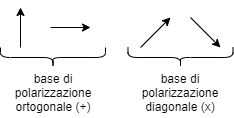
\includegraphics[width=150px]{QDK_1.png}
\end{figure}

La direzione di polarizzazione può essere qualsiasi quindi scegliamo una base per rappresentarla (come se fosse un vettore).
In ognuno di questi stati codifichiamo un bit:
\begin{itemize}
    \item verticale: 0
    \item orizzontale : 1
    \item +45°: 0
    \item -45°: 1
\end{itemize}

NB: Perché due basi? Se ne usassimo una sola potremmo misurare perfettamente lo stato, se invece non so quale base abbiamo usato non posso effettuare misurazioni corrette e certe ma solo probabilistiche, noi ci basimo proprio su questa probabilità!

Vediamo la struttura generale dell' hardware necessario:

\begin{figure}[H]
    \centering
    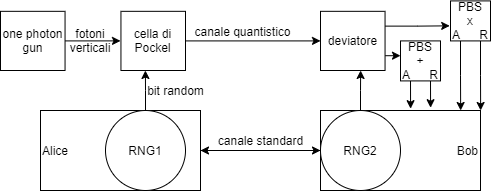
\includegraphics[width=300px]{QDK_2.png}
\end{figure}

Ci si muove su due canali, uno quantistico (fibra ottica) ed uno standard. Solo uno dei due trasmette sul quantistico. Si utilizzano:
\begin{itemize}
    \item One Photon Gun: emette singoli fotoni tutti verticali
    \item Cella di Pockel: impone una determinata polarizzazione scelta dal RNG1
    \item PBS (beam splitter polarizzante): ci da corretta polarizzazione del fotone se e solo se la base di generazione e la base di misurazione sono le stesse. Misura il fotone tramite la deviazione verso una delle due uscite: A (assorbimento) ed R (riflessione).
    Quando il fotone esce, esce con una delle due polarizzazioni misurabili dal PBS, non importa più quella originale.
\end{itemize}

Sia $\theta$ l'angolo tra la base di polarizzazione di misurazione e la polarizzazione del fotone stesso, allora si hanno:
\begin{itemize}
    \item esce da A con probabilità $cos^2 \theta$
    \item esce da R con probabilità $sin^2 \theta$
\end{itemize}

Si noti quindi che:
\begin{itemize}
    \item se la base di misurazione e la base di generazione sono identiche il fotone mantiene la polarizzazione
    \item se le basi di misurazione e di generazione sono diverse $\theta = \pm45^{\circ}$ quindi $cos^2\theta = sin^2\theta = \frac{1}{2}$ quindi il fotone ha pari probabilità di uscire da A o da R.
\end{itemize}

La lettura attraverso il PBS quindi potrebbe distruggere lo stato quantistico precedente:
\begin{table}[ht!]
    \centering
    \begin{tabular}{c|c|c|c|c}
        & 0 $\uparrow$ & 0 $\nearrow$ & 1 $\rightarrow$ & 1 $\searrow$ \\
        \hline
        + & $\uparrow$ & $\uparrow \rightarrow$ & $\rightarrow$ & $\uparrow \rightarrow$  \\
        x & $\nearrow \searrow$ & $\nearrow$ & $\nearrow \searrow$ & $\searrow$
    \end{tabular}
\end{table}

Andiamo dunque al protocollo:
\begin{itemize}
    \item Alice si segna le basi usate per generare i fotoni: $S_A$
    \item Bob si segna quali basi ha usato per effettuare le misure: $S_B$
    \item Bob invia ad Alice le sue basi (sul canale standard)
    \item Alice risponde dicendo quali basi sono corrette
    \item Dove le basi sono concordi si prendono i bit, dove le basi sono discordi si buttano.
    Si ha circa il 50\% di match
\end{itemize}

In assenza di interferenze di Eve, Alice e Bob possiedono $S_A' = S_B'$ sottosequenze identiche formate dai bit codificati e decodificati con basi comuni:
$$ \mid S_A' \mid = \mid S_B' \mid = \frac{\mid S_A \mid}{2} $$

\begin{table}[ht!]
    \centering
    \begin{tabular}{c|c c c c c c c c | c}
        Alice: & 1 & 0 & 1 & 1 & 1 & 0 & 0 & ... & $S_A$ \\
        Alice: & + & x & + & x & x & + & x & ... & basi di A \\
        invia: & $\rightarrow$ & $\nearrow$ & $\rightarrow$ & $\searrow$ & $\searrow$ & $\uparrow$ & $\nearrow$ & ... & fotoni di A \\
    
        & & & & & & & & & \\

        Bob: & + & x & + & + & + & x & x & ... & basi di B \\
        Bob: & $\rightarrow$ & $\nearrow$ & $\rightarrow$ & $\uparrow$ 50\% & $\rightarrow$ 50\% & $\searrow$ 50\% & $\nearrow$ & ... & letture di B \\
        Riceve: & 1 & 0 & 1 & 0 & 1 & 1 & 0 & ... & $S_B$ \\
    \end{tabular}
\end{table}

Le basi concordi sono 1, 2, 3, 7 che portano alla sequenza:
$$ S_A' = S_B' = 1010 $$

Se c'è un crittoanalista esso si troverà nella stessa situazione di Bob, quindi deve scegliere le sue basi.
Le basi che sceglierà saranno indipendenti da quelle di Alice e Bob quindi se la sua base coincide con quella di Alice non cambia nulla, invece se non coincide altera irreparabilmente il fotone!
Alice e Bob fanno quindi una verifica: sacrificano un pezzo si $S_A'$ e $S_B'$:
si scambiano una porzione delle chiavi comuni in posizioni prestabilite comunicandole sul canale standard.
Se le due sequenze sono diverse allora interrompono la comunicazione.
Altrimenti usano la porzione rimanente come chiave o per costruire la chiave.


\begin{table}[ht!]
    \centering
    \begin{tabular}{c|c c c c c c c c}
        Alice: & 1 & 0 & 1 & 1 & 1 & 0 & 0 & ... \\
        Alice: & + & x & + & x & x & + & x & ... \\
        invia: & $\rightarrow$ & $\nearrow$ & $\rightarrow$ & $\searrow$ & $\searrow$ & $\uparrow$ & $\nearrow$ & ... \\
    
        & & & & & & & & \\

        Eve: & + & + & + & x & + & x & + & ... \\
        Eve: & $\rightarrow$ & $\rightarrow$ 50\% & $\rightarrow$ & $\searrow$ & $\uparrow$ 50\% & $\nearrow$ 50\% & $\rightarrow$ 50\% & ... \\
        Riceve: & 1 & 1 & 1 & 1 & 0 & 0 & 1 & ... \\

        & & & & & & & & \\

        Bob: & + & x & + & + & + & x & x & ... \\
        Bob: & $\rightarrow$ & $\searrow$ 50\% & $\rightarrow$ & $\uparrow$ 50\% & $\uparrow$ & $\nearrow$ & $\searrow$ 50\% & ... \\
        Riceve: & 1 & 1 & 1 & 0 & 0 & 0 & 1 & ... \\
    \end{tabular}
\end{table}

Prendiamo i valori con basi concorde:
$$ S_A' = 1010 \neq S_B' = 1111 $$

Supponiamo quindi che si sacrifichi il secondo bit: $0 \neq 1$ e quindi ci si accorge di una intrusione.

I bit non perturbati sono quelli per cui le 3 basi coincidono: $\frac{1}{4}$ delle volte.
Quindi se Eve interviene: circa la metà di $S_A'/S_B'$ sarà differente.
La verifica dell'intrusione è quindi importantissima, permette di sapere di eventuali intrusioni e quindi evitare di perdere informazioni.

Ci sono comunque degli errori generici in fase di trasmissione dei fotoni, delle letture, ecc.
Si stabilisce quindi un \emph{quantum bit error rate} - QBER: una percentuale prevedibile di bit errati (dovuti a errori dell'apparato sperimentale).
Se quindi nel confronto tra $S_A''$ e $S_B''$ il numero di errore è $>$ QBER allora c'è stata una intromissione, altrimenti sono solo errori sperimentali e si correggono tramite correttori di errori.

NB: Eve potrebbe intercettare pochi fotoni e quindi farsi passare per errori dell'apparato pur conoscendo alcuni bit della chiave.
Proprio per questo motivo anziché usare la sequenza scambiata si usa farne l'hash ed usare quello come chiave, in quato modo se cambiano anche solo pochi bit l'hash cambia enormemente.


NB: le comunicazioni su canale standard possono anche essere in chiaro, è bene tuttavia che siano autenticate, magari tramite MAC (simmetrico con chiave scambiata in anticipo).

\subsection{Variante}
Esiste un altro algoritmo quantistico di scambio di chiavi che si basa sull'entanglement.
Se i due estremi misurano con la stessa base fotoni correlati sono correlati anche i loro risultati quindi A e B misurano chiavi complementari.

\section{Bitcoin}

Non è propriamente una moneta, è un sistema di pagamento.
Sfrutta protocolli crittografici sia per generare nuova moneta che per attestare il possesso della valuta da parte degli utenti.

Nasce nel 2008 con la pubblicazione di \emph{Bitcoin: a peer to peer Electronic cash system} a cura di \emph{Satoshi Nakamoto} (pseudonimo per una persona o un gruppo ancora ignoto).
Nel 2009 viene rilasciato il primo software per partecipare (bitcoin-core) ed il 3 Gennaio 2009 viene creato il \emph{blocco genesi}.

Questo sistema è costituito da un libro contabile (\emph{ledger}) pubblico e distribuito costituito da singoli blocchi concatenati tra di loro: la \emph{blockchain}.
Con il primo blocco si sono creati i primi 50 bitcoin.
Ogni volta che si riesce ad aggiungere un nuovo blocco si creano nuovi bitcoin ed ogni 4 anni circa si dimezza la moneta generata (inizialmente 50 bitcoin per blocco, ora 6.25 per blocco).
La generazione ha un tempo massimo infatti nel 2140 l'aggiunta di blocchi non genererà più nuova moneta.

Il 12 Gennaio 2009 avviene la prima transazione: Satoshi Nakamoto invia 10 Bitcoin ad Hal Finney (il creatore del proof of work).

Nel 2010 avviene la prima transazione commerciale, vengono pagate due pizze.

\subsection{Come funziona?}
Dopo aver scaricato il software necessario l'utente genera una sua coppia di chiavi pubblica e privata:
\begin{itemize}
    \item $K_A[pub]$: costituisce l'indirizzo identificativo dell'utente, si usa per ricevere Bitcoin e per verificare la firma
    \item $K_A[priv]$: si usa per firmare le transazioni e quindi spendere
\end{itemize}

\subsubsection{Wallet}
E' l' insieme delle credenziali che attestano la proprietà in BTC di un utente: la coppia indirizzo/chiave privata in quanto ogni utente ne possiede una assieme al software di gestione

\subsubsection{Transazione}
E' lo scambio di valuta tra due utenti. Immaginiamo che A voglia inviare $x$ BTC a B: il messaggio avrà la forma:
$$ m = address_A - x - address_B$$
verrà corredato da un hash:
$$ h = SHA-256(m)$$
e dalla firma:
$$ f = D(h, K_A[priv]) $$
la coppia $<m, f>$ verrà quindi diffusa nella rete peer-to-peer in broadcast.

Essendo su un sistema distribuito il destinatario deve aspettare che la rete convalidi la transazione e richiede almeno 10 minuti.
Dopo 10 minuti il blocco verrà aggiunto alla blockchain, bisogna poi aspettare l'aggiunta di altri 6 blocchi al nostro ramo per essere sicuri al 100\% di aver compiuto una transazione.

All'interno di una transazione i bitcoin non possono essere frazionati:
\begin{table}[ht!]
    \centering
    \begin{tabular}{c c c}
         &  & 0.5 Bitcoin ad Alice \\
        Bob riceve 50 Bitcoin &  $\xrightarrow{transazione A}$ &\\
         & & 49.5 Bitcoin a Bob
    \end{tabular}
\end{table}

Successivamente Alice può spendere o meno i bitcoin ricevuti.
Può anche mettere assieme più indirizzi di input:
\begin{table}[ht!]
    \centering
    \begin{tabular}{c c c}
        Alice riceve 0.5 Bitcoin & & \\
        Alice riceve 0.1 Bitcoin & $\xrightarrow{transazione B}$ & utente riceve 0.8 Bitcoin\\
        Alice riceve 0.2 Bitcoin & &
    \end{tabular}
\end{table}

Si possono spendere solo output non spesi di precedenti transazioni che avevano noi come destinatario.
La somma degli input deve sempre essere maggiore o uguale alla somma degli output, se è uguale pagamenti normali, se è maggiore quelli in più viene aggiunto al primo che convalida il blocco (perché può aggiungere questo movimento).
Per incentivare questo conferma si usa quindi lasciare questa fee al miner.

\subsubsection{Validazione}
Gli utenti ricevono dal broadcast queste transazioni, le controllano (cercano nel passato se la valuta è presente nel conto di chi invia) le mettono assieme a gruppi (100, 200 anche 1000) e poi provano ad aggiungerle alla blockchain.
Ci sono vari modi per aggiungerli, noi vedremo il \emph{proof of work}.

Tutto questo è fatto per evitare che sia possibile il double spending: creare più transazioni quasi contemporaneamente, questo potrebbe succedere nel periodo in cui avviene la validazione, ma si risolve con questa divisione in blocchi.

\subsection{Com'è fatto un blocco}

\begin{figure}[H]
    \centering
    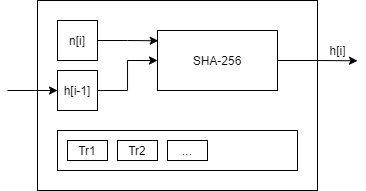
\includegraphics[width=300px]{Bitcoin_1.png}
\end{figure}

Prendo un tot di transazioni, le raggruppo, aggiungo la transazione finale che mi dirige la ricompensa, costruisco la porzione $Tr_{i}$.

Nel blocco c'è $h_{i-1}$ cioè l'hash del blocco precedente. Nel blocco c'è $n_i$ detto \emph{nonce}, un intero.

Di queste informazioni faccio l'hash SHA-256 ed ottengo $h_i$. La richiesta è quella di ottenere un $h_i < $ di una certa soglia fissata dal sistema.
Ciò che si fa è quindi iterare su tutti i nonce e cercare un hash con $T$ zeri all'inizio.
Il parametro $T$ è fissato dal sistema e varia in base alla potenza della rete.
Questo è scelto in modo da portare il tempo di validazione di un blocco a circa 10 minuti.
In media ci vogliono $2^T$ tentativi.

Chi cerca di attaccare un nuovo blocco è detto \emph{miner} e sono i nodi che validano le transazioni.

Si parla di \emph{validazione tramite mining}.

Cercare il nonce è difficile, verificarlo invece è semplice quindi chi trova il nonce lo diffone in broadcast a tutti i nodi, gli altri lo verificano, controllano la validità delle transazioni ed esprimono il loro consenso: prendono il nuovo nodo e cercheranno di attaccare nuovi nodi ad esso.

Se la rete ad un certo punto ha delle biforcazioni si tende a privilegiare i rami con più transazioni perché è più probabile che siano accettati da tutta la rete.

La proof of work è quindi questa ricerca del nonce.

\subsection{Mining pool}
Inizialmente Bitcoin doveva essere democratico e quindi tutti avrebbero potuto partecipare al mining, quello che è successo invece è stato che alcuni piccoli gruppi di utenti hanno unito le forze e messo a disposizione grande hardware per minare tutti assieme, ci si spartisce quindi lo spazio di ricerca del nonce e si dividono i profitti tra i vari partecipanti.

\subsection{Aspetti sociali}
Il mining ormai è poco sociale in quanto lo fanno in pochi e guadagnagno in pochi.
Inoltre si perde un sacco di energia elettrica per calcoli "inutili".
Sono state quindi sviluppate altre monete digitali che dirigono il proof work verso ambiti di ricerca per non rendere tutta questa energia elettrica sprecata

\subsection{Attacchi alla blockchain}
Per attaccare la blockchain si deve disporre di una grande potenza di calcolo.
Si possono mettere d'accordo più persone per far si che si attacchino blocchi a piacere.
Si deve disporre del 51\% della rete che è abbastanza difficile, se avessi questa potenza però sarebbe più remunerativo giocare onestamente.














\end{document}